
\emptypage

% ============================================================================
%  Ackowledgements
% ============================================================================
\chapternonum{Acknowledgements}
%\chapter{Acknowledgements}

%thank you 'n stuff

\emptypage

% ============================================================================
% Table of contents
% ============================================================================

\singlespace
\dominitoc
\renewcommand{\leftmark}{Contents}

\tableofcontents

\emptypage

% ============================================================================
%   Introducton
% ============================================================================

\onehalfspacing
\setcounter{page}{1}
\pagenumbering{arabic}
%\chapternonum{Introduction}
%\chapter{Introduction}

%\vspace*{0.5cm}

\chapternonum{Introduction}

The knowledge about particle physics brought us many inventions widely used and appreciated in the society. The particle physics applications are now used in many fields, from medicine to the energy industry. To further understand and broaden our knowledge about the elementary particles and interactions, the Large Hadron Collider was built at CERN. The Large Hadron Collider is providing particle collisions in four detectors, one of them being the Compact Muon Solenoid~(CMS). In the detector the colliding particles interact, leading to the creation of new particles.  The created particles are traversing the detector and leaving there the energy deposits along their path. To be able to reliably reconstruct the picture about what happened in the detector, precise measurement of these deposits is vital.

The first Chapter~\ref{sec:detch} briefly introduces the Large Hadron Collider and Compact Muon Solenoid, giving more detailed information about areas which are further developed in the following chapters. This chapter also discusses the reconstruction of the physics objects seen in the detector.

In Chapter~\ref{sec:HIPch} we discuss the CMS strip tracker and observed inefficiencies during years 2015 and 2016, in the reconstruction of particle paths due to its inability to measure the energy deposits. This effect was believed to be caused by the inelastic nuclear interactions in the sensitive volume of the tracker, which lead to the saturation of the tracker electronics. This chapter presents results on the probability of the nuclear interactions and effects resulting from such interactions. 

The third chapter, Chapter~\ref{ch:simu}, focuses as well on the CMS silicon tracker, but in this case on its simulation. In order to be able to compare the results of the experiment with the theoretical expectations, the simulation of the interactions of particles generated according to the theoretical model with the detector must be simulated. This chapter describes how the simulation in the strip tracker is implemented and how it can be improved. At the end we present results on measurement of the tracker properties which are taken as a parameters in the simulation. We show how introducing these parameters into simulation improve the description of data by simulation at the level of the energy deposits.

The particle physics is described by the standard model, which last piece, the Higgs boson, was discovered in 2012 by the CMS and ATLAS collaborations. Although the standard model is now complete and in general well describing the physics phenomena, it suffers from several shortcomings. This issue makes us believe that the standard model is an effective theory, which is a part of a bigger theory. Over years, many theories  were proposed and one, referred to as supersymmetry, became of a special interest due to its capability to address many of the standard model shortcomings. Both standard model and supersymmetry are discussed in Chapter~\ref{sec:SUSYch}.

The supersymmetry introduces a new partner to each standard model particle and therefore extensive searches for these particles are performed by the CMS and other collaborations. One of these particles is a supersymmetric partner of the top quark which is expected to have a mass around 1~TeV and therefore be accessible at the LHC energies. The last chapter before conclusion, Chapter~\ref{sec:stopch},  presents search for this supersymmetric partner of the top quark in the single lepton final state.


%particle physics studies the 
% particles building blocks of the matter around us
%to understand this matter and interaction between the particles
%-> LHC and experiments 

%to be able to study these particles we need well performing detector
%detector - cahpter one
%HIP - discusssed in the second chapterr
%then 

%stop chapter 3

%with the discovery of the Higgs boson, the standard model became complete, but still many puzzles persisted
%SM effective theory weell describing our world
%SUSY to target the SM problems chapter 4
% chapter 5
%stop expected to eb relatively light
%touchinh anturality bound, but there are still many corners unsearched

\clearpage

\setcounter{secnumdepth}{4}
\chapterwithnum{The CMS experiment at the LHC~\label{sec:detch}}
\setcounter{secnumdepth}{5}

There are several options how to study elementary particles, for example it can be studied via cosmic rays, astrophysical neutrinos, direct searches for the dark matter or at collider experiments. In Section~\ref{sec:LHC} the largest existing collider, the LHC, and its experiments are introduced. In Section~\ref{sec:CMS} the CMS detector, in which context this thesis is performed, is described. Then in Section~\ref{sec:objects}, the object reconstruction techniques of the CMS collaboration applied on the CMS data are introduced. A special interest is put on the topics whose a deeper understanding is required for the following chapters of this thesis.

\section{The Large Hadron Collider~\label{sec:LHC}}

The Large Hadron Collider~(LHC)~\cite{Evans:2008zzb} is a particle accelerator with a circumference of 27~km, which is a part of the CERN accelerator complex~\cite{Bruning:2004ej} located near Geneva, Switzerland. The LHC project was approved in 1994 and designed to provide mainly collisions of protons. Part of the LHC operation time is also dedicated to collisions of heavy nuclei, but in this thesis only the proton collisions are described.

A schematic view of the CERN accelerator complex with its main experiments is presented in Fig.~\ref{fig:figures/CCC-v2016}~\cite{Mobs:2225847}. At the beginning of the acceleration process the protons are obtained by stripping electrons from the hydrogen atoms. Protons are then accelerated through a chain of accelerators: Linac2, Booster, Proton Synchrotron~(PS) and Super Proton Synchrotron~(SPS). The proton beams accelerated to 450~GeV are injected from the SPS into the LHC using separate pipes, one beam turning clockwise and the other one anti-clockwise. In the LHC, the beams are further accelerated with eight radio-frequency~(RF) cavities per beam, currently to the beam energy of 6.5~TeV. The LHC is equipped with 9593 magnets, mainly dipoles and quadrupoles, to bend and focus the beams. There is an ultrahigh vacuum of order of $10^{-10}-10^{-11}$~mbar in the LHC tube to avoid collisions of particles with gas. A vacuum of around $10^{-6}$~mbar is also used for the isolation  of cryomagnets and the helium distribution line.

    \insertFigure{figures/CCC-v2016} % Filename = label
                 {0.99}       % Width, in fraction of the whole page width
                 { The CERN accelerator complex~\cite{Mobs:2225847}. }

The proton beams are not homogeneous but composed of trains of bunches, each bunch containing around 100 billions of protons. Bunches within a given train are spaced by 25~ns. Time gaps between two different trains are longer, their duration depends on the beam structure and \textcolor{red}{currently they start from seven times 25~ns}. The LHC uses several beam structures, which are specified by the filling scheme. An example of a beam structure is shown in Fig.~\ref{fig:figures/beamStructure}. 

Up to now, the LHC operation has been divided into two eras, Run~1 and Run~2. The Run~1 started in 2008 and ended in 2013. During this era the center-of-mass energy of the pp collisions was first 7~TeV, then it was increased to 8~TeV in 2012, and the beam structure allowed collisions every 50~ns. The Run~2 started in 2015 and is still ongoing. In the Run~2 the collision center-of-mass energy increased to 13~TeV and the time between collisions was reduced to 25~ns. The Run~2 stops at the end of 2018, the Run~3 is scheduled to start in 2021.

    \insertFigure{figures/beamStructure} % Filename = label
                 {0.8}       % Width, in fraction of the whole page width
                 { (top) An example of beam structure. The beam pipes are shown in red and violet and the beams are drawn in green. (bottom) An example showing the structure of two trains. }

The bunches of protons collide at four interaction points (IP), at which four main experiments are installed. The two general-purpose detectors, which are designed to cover a wide range of physics, are ATLAS (standing for ``A Toroidal  LHC ApparatuS'')~\cite{Aad:2008zzm} and CMS (standing for ``Compact Muon Solenoid'')~\cite{Chatrchyan:2008aa}. The other two main experiments are ALICE (standing for ``A Large Ion Collider Experiment'')~\cite{Aamodt:2008zz}, mainly focusing on the physics of heavy-ion collisions and the study of the ``quark-gluon plasma'' which existed at the early Universe, and the LHCb (standing for ``Large Hadron Collider beauty'')~\cite{Alves:2008zz} specialized in the physics of the b-quark. There are also three smaller experiments along the LHC, one of them is TOTEM~\cite{Anelli:2008zza} which is close to CMS and its principal goal is to measure the total cross section of protons at the LHC. LHCf~\cite{Adriani:2008zz}, which is located near to the ATLAS experiment, studies particles moving very close to the proton beams. Finally MoEDAL~\cite{Acharya:2014nyr}, which is close to LHCb, focuses on the search of hypothetical particles, e.g. magnetic monopoles.

One of the main motivations for the LHC and its experiments was the search for the Higgs boson. After its discovery in 2012 by the ATLAS and CMS collaborations, the measurement of the Higgs boson properties has now entered into the physics program. A second important topic of research is the search for new particles and more generally for evidence of physics beyond the Standard Model, motivated mainly by cosmological observations, naturalness of the Higgs mass and the desire for unification of known interactions.

%\newpage

%TODO here

\section{The Compact Muon Solenoid detector~\label{sec:CMS}}

%The CMS (``Compact Muon Solenoid'') detector~\cite{Chatrchyan:2008aa, CMSproposal} is a multipurpose detector of overall length of 22~m, a diameter of 15~m and a weight of 14~t, located at the IP~5. The designed properties of the CMS  detector were to have high efficiency of muon identification and reconstruction. It was also required have precise momentum resolution in large range of momenta, dimuon mass resolution of order of 1\% at 100 GeV, good charged-particle momentum measurement and resolution~(around 1\%-2\% for 10~GeV muons in majority of CMS coverage) as well as high efficiency in reconstruction of charged-particle tracks. Furthermore it was designed to have precise measurement electromagnetic energy, leading to resolution of diphoton and dielectron mass of around 1\% at 100~GeV. Good missing transverse energy~(MET) and dijet mass resolution was required as well. One of the important requirements was also high efficiency in offline tagging of tau particles and jets originating from b-quarks. These conditions have to be fulfilled in the LHC environment, with a bunch crossing~(BX) frequency of 25~ns, where every bunch crossing leads to tens of inelastic interactions on top of the interaction of the interest, referred to as ``pileup''~(PU), resulting in thousands of charged particles in the CMS detector every 25~ns. Because of this large radiation, the detectors and front-end electronics have to be radiation-hard.

The CMS (``Compact Muon Solenoid'') detector~\cite{Chatrchyan:2008aa} is a multipurpose detector of an overall length of 22~m, a diameter of 15~m and a weight of 14~t, located at the IP~5. The designed properties~\cite{CMSproposal} of the CMS  detector were to have high a quality tracking providing precise charged-particle momentum measurement and resolution around 1\%-2\% for 10~GeV muons in the majority of the CMS coverage being $\abs{\eta}<2.4$ and to have high efficiency of muon identification and reconstruction, leading to a requirement on  a dimuon mass resolution of the order of 1\% at 100 GeV. Furthermore it was designed to have the best possible measurement of the electromagnetic energy, leading to a resolution of diphoton and dielectron masses of around 1\% at 100~GeV. These conditions have to be fulfilled in the LHC environment, with a bunch crossing~(bx) every 25~ns, where every bunch crossing leads to tens of inelastic interactions on top of the interaction of the interest, referred to as ``pileup''~(PU), resulting in thousands of charged particles in the CMS detector every 25~ns. Because of this large radiation, the detectors and front-end electronics have to be radiation-hard.

To achieve the given requirements, CMS was built in layers around a large solenoidal magnet, with endcaps at each side. The CMS magnet is a superconducting solenoid providing a magnetic field of 3.8~T. The magnet is surrounded from outside by the steel yoke which returns the magnetic flux of the solenoid~\cite{tdrMagnet}. The radius of the magnet has to be kept relatively small and therefore the available space between the magnet and interaction point is limited.

Inside the magnet from the interaction point outwards, there is a pixel and silicon strip tracker, followed by the electromagnetic and hadron calorimeters. Outside of the magnet there is the outer hadron calorimeter and the steel return yoke with embedded muon chambers. The CMS detector layout is shown in Fig.~\ref{fig:figures/cmsdetector}~\cite{website:CMSdet}. In the following sections, first the coordinate system of the CMS is described. Then the CMS subdetectors are introduced, starting from the innermost one. At the end, basic information on trigger, luminosity and pileup is given.
%-coverage up to |eta|<5


    \insertFigure{figures/cmsdetector} % Filename = label
                 {0.99}       % Width, in fraction of the whole page width
                 { A schematic layout of the CMS detector~\cite{website:CMSdet}. }

\subsection{Coordinate system and conventions}


The coordinate system used by CMS~\cite{Chatrchyan:2008aa} is sketched in Fig.~\ref{fig:figures/coordinates}~\cite{Pantaleo:2293435}. In the CMS conventions, the cartesian coordinate system is centered at the IP, with the x-axis pointing into the center of the LHC, the y-axis going upwards and the z-axis going anti-clockwise along the beam direction. The azimuthal angle $\Phi$ is defined in the x-y plane and is measured from the x-axis. The polar angle $\theta$ is measured from the z-axis and is defined in the y-z plane. Finally $r$ is a radial coordinate in the x-y plane. In this convention the pseudorapidity $\eta$ is defined as

\eq{pseudorapidity}
{
    \eta =  -\ln \left[ \tan \left( \frac{\theta}{2} \right) \right].
}

The angular distance between two points can be measured with the help of $\Delta R$ defined as

\eq{deltaR}
{
    \Delta R = \sqrt{ \Delta \Phi^2 + \Delta \eta^2}.
}


The transverse momentum $p_{T}$ can be computed from the x and y momentum components as

\eq{pseudorapidity}
{
    p_{T} =  \sqrt{p_{x}^2 + p_y^2 }.
}

\textcolor{red}{At the interaction point, the partons in proton beams have negligible momentum in the x-y plane, and therefore  } the sum of momenta of all particles originating from the collision in this plane should be zero due to momentum conservation law. Therefore an imbalance of momenta in this plane, i.e. a non-zero total $p_{T}$, can be a sign of particles whose momentum is unmeasured, like neutrinos or hypothetical new particles. 

    \insertFigure{figures/coordinates} % Filename = label
                 {0.6}       % Width, in fraction of the whole page width
                 { The CMS coordinate system with the three axes intercepting at the interaction point, the x-axis pointing inside the LHC ring, the y-axis going upwards and the z-axis pointing anti-clockwise along the beam~\cite{Pantaleo:2293435}. }

\subsection{The silicon tracker~\label{sec:tracker}}

The silicon tracker~\cite{CMS:1997tlf, CMS:2000eqx} is the innermost subdetector of the CMS detector. The CMS tracker is divided into two parts, the inner (outer) part consists of a pixel (strip) detector.  Its purpose is to reconstruct tracks from charged particle depositions, energy losses $E_{loss}$, in silicon sensors. In order to recognize from which interaction a given particle originates, the tracker is required to have a capability to reconstruct primary and secondary vertices. The reconstruction of primary vertices targets to find the positions where the interaction of interest or the PU interaction occurred. The primary vertices are determined by the vertex fitting procedure from the tracks~\cite{Ball:2007zza}. The goal of the secondary vertex reconstruction is to spot the place where a particle with a long lifetime decays to other particles. 

On the tracker level, the tracking is performed in 4 steps~\cite{website:slidesTracking, website:twikiTracking}. It starts from  hits reconstructed from particle depositions in the sensors. First, the \textit{track seeding} is performed from three 3-D reconstructed hits \textcolor{red}{ in pixel and/or strip tracker} or two of them with a constraint on the beam spot. Then the algorithm proceeds with \textit{track building} which aims to connect all hits originating from one particle. During the track building the track is propagated to the neighboring layers of the tracker, testing the compatibility of the reconstructed hit with the track by a $\chi^{2}$ test. Once the full track candidate is complete, the \textit{track fitting} is performed to obtain the best parameters of the track and to recompute precisely the hit position using the track properties. The last step is a \textit{track quality selection} rejecting tracks not fulfilling quality requirements, which are based on the $\chi^{2}$ of the final fit, the number of layers with a hit associated to the track and the probability of the track  to originate from the primary vertex.

The default track reconstruction~\cite{Chatrchyan:2014fea} is using the software referred to as the Combinatorial Track Finder~(CTF), based on the combinatorial Kalman filter~\cite{Fruhwirth:1987fm}. The tracking uses an iterative approach: in the first iteration the easiest tracks to find are reconstructed (i.e. the ones with the highest $p_{T}$), then after these tracks are complete their hits are masked in order to avoid duplicities and reduce combinatorics for further iterations of tracks finding. In total there are 12 iterations and each iteration is focused on a specific type of tracks.


Due to the presence of the magnetic field, charged particles are bent according to their momentum and charge, thus the CMS tracker is able to measure the charge sign and the momentum associated to a track. To perform so, the tracker needs to have a good spatial resolution. It has to be as well extremely radiation-hard due to the large flux of incoming particles. Also the material was chosen carefully, in order to reduce multiple scattering, nuclear interactions or bremsstrahlung in the tracker material.

The flux of particles in the CMS detector decreases with the distance from the interaction point, the flux of charged particles in the barrel at a radius of 4~cm is around $10^{8}~\mathrm{cm^{-2}s^{-1}}$ while at a radius of 115~cm it decreases to around $3 \times10^{5}~\mathrm{cm^{-2}s^{-1}}$. Consequently, the inner part of the tracker is made of silicon pixels, which are able to measure particle paths and their properties in a high particle density environment. Moreover a good resolution is needed for the vertex determination. In the outer part of the tracker, the particle density is low enough to use silicon strip sensors, which are cheaper mainly because they require less readout channels. Overall, the tracker pseudorapidity coverage is  $|\eta| < 2.5$.


\textbf{The silicon pixel tracker}

%The silicon strip tracker is 5.8~m long with a diameter of 2.5~m. 
Before 2017, the pixel barrel, referred to as BPIX,  was located at a radius of 4.4~cm up to 10.2~cm, from the IP. The pixel endcaps~(FPIX) extended on each side from 35~cm to 47~cm in the z direction. In total, there were three barrel layers and two endcaps layers on each side. During an extended winter shut-down in 2017, due to the high radiation exposure, the pixel tracker was replaced. The new pixel tracker has four barrel layers covering 3$\leq r \leq$16~cm and three endcap disks at distances  29.1$\leq \abs{z} \leq$51.6~cm. The pixel detector plays a crucial role in the track seeding, and the reconstruction of the primary and secondary vertices~\cite{CMS:2012sda}. 


%-new pixels - short distance from IP, high radiation -> damage -> need for replacement
%- FPIX - 3 disks on each side 29.1cm -51.6cm  (Forward pixel) ~\cite{CMS:2012sda}
%- BPIX - barrel pixel - 4 cylindrical layers radius of 3-16 cm

\textbf{Silicon strip tracker}

%15148 silicon strip modules

As the following chapters present studies of the silicon strip tracker and its simulation, let take now a deeper look into its design and properties. The silicon strip tracker is divided into four partitions. Each partition is composed by several layers of modules, which have either one side~(mono) or two sides~(stereo) of silicon sensors. In total the strip tracker is composed of 15148 modules. The Tracker Inner Barrel~(TIB) is the innermost barrel part with two layers of stereo modules succeeded by two layers of mono modules. The Tracker Outer Barrel~(TOB) surrounds the TIB. In the innermost part of TOB, there are two layers of stereo modules, the remaining four layers being mono. On each side of the barrel, Tracker Inner Disks~(TID) and Tracker EndCaps~(TEC) are located. There are three wheels (perpendicular to the z-axis) of TID with three module rings (parallel to the z-axis) and 9 wheels of TEC with four to seven rings of modules on each side. In each wheel there is a mixture of mono and stereo modules, but each ring has either mono or stereo modules. 

In the barrel region, the silicon tracker is placed in radius between 20~cm up to 1.1~m from the IP. The disks start at 80~cm in the z-direction from the IP and the endcaps reach up to z=2.8~m from the IP. The overall layout of the silicon strip tracker can be seen in Fig.~\ref{fig:figures/cmsTracker}~\cite{Chatrchyan:2014fea}.

    \insertFigure{figures/cmsTracker}
                 {0.9}       
                 {A schema of the longitudinal view of the upper half of the CMS silicon strip tracker and layout of its partitions. The star represents the IP. The modules in blue are stereo, while the mono ones are shown in black~\cite{Chatrchyan:2014fea}. }

Each mono module holds 320~$\mathrm{\mu m}$ or 500~$\mathrm{\mu m}$ thick silicon sensors with either 512 or 768 silicon strips.  The strip length range is from 8 to 25~cm. The distance between strips, called pitch, varies between around 80~$\mathrm{\mu m}$ and 200 ~$\mathrm{\mu m}$.  In the barrel, the strips are parallel to the z-axis, or tilted by 100~mrad with respect to the z-axis in case of the stereo sensors. In TID and TEC, the strips \textcolor{red}{are not parallel to each other and} are aligned to be parallel to $r$, \textcolor{red}{or tilted by 100~mrad with respect to the $r$ in case of the stereo sensors}. The strip width to pitch ratio is equal to 0.25.

The local module coordinates have their zero in the middle of the module, the z-axis going in the direction from the back-plane to the strips, the y-axis going along the strips, and the x-axis being perpendicular to the strips and traversing them. The local $\theta$ angle is measured from the z-axis. The local $\Phi$ is defined in the x-y plane and measured from the x-axis. The schematic view of the sensor local coordinates is shown in Fig.~\ref{fig:figures/localCoordinates}. The details about the module geometries for each layer of TIB and TOB and each ring of TID and TEC can be found in Table~\ref{tab:trackerGeometries}~\cite{website:hephyPage}.


    \insertFigure{figures/localCoordinates} % Filename = label
                 {0.6}       % Width, in fraction of the whole page width
                 { The sensor local coordinate system with the three axes intercepting in the middle of the sensor. The x-axis is perpendicular to the silicon and aluminium strips (represented by the dark gray bands on the top of the drawing), the y-axis goes along the strips and the z-axis points from backplane (represented at the bottom by the dark gray/green surface) to the strips. }

\begin{table}[h]
\begin{center}
\begin{tabular}{|l|l|l|l|l|l|}
\hline
Layer & Type  & \#Strips & Thickness~[$\mathrm{\mu m}$] & Pitch~[$\mathrm{\mu m}$] & Geometry label  \\
\hline
\hline
TIB L1 & stereo & 768 & 320 & 80 & IB1 \\
TIB L2 & stereo & 768 & 320 & 80 & IB1 \\
TIB L3 & mono & 512 & 320 & 120 & IB2  \\
TIB L4 & mono & 512 & 320 & 120 & IB2 \\
\hline
TOB L1 & stereo & 768/512 & 500 & 122/183 & OB2 \\
TOB L2 & stereo & 768/512 & 500 & 122/183 & OB2  \\
TOB L3 & mono & 512 & 500 & 183  & OB2 \\
TOB L4 & mono & 512 & 500 & 183  & OB2 \\
TOB L5 & mono & 768 & 500 & 122  & OB1 \\
TOB L6 & mono & 768 & 500 & 122  & OB1 \\
\hline
TID R1 & stereo & 768 & 320 & 81...112  & W1a \\
TID R2 & stereo & 768 & 320 & 113...143 & W2a  \\
TID R3 & mono & 512 & 320 & 124...158  & W3a \\
\hline
TEC R1 & stereo & 768 & 320 & 81...112 & W1b  \\
TEC R2 & stereo & 768 & 320 & 113...143 & W2b   \\
TEC R3 & mono & 512 & 320 & 124...158  & W3b \\
TEC R4 & mono & 512 & 320 & 113...139  & W4 \\
TEC R5 & stereo & 768 & 500 & 126...156  & W5 \\
TEC R6 & mono & 512 & 500 & 163...205  & W6 \\
TEC R7 & mono & 512 & 500 & 140...172  & W7 \\
\hline
\end{tabular}
\caption[Table caption text]{Module type, strip multiplicity, sensor thickness and pitch and module geometry label for layers or rings of the four silicon strip tracker partitions~\cite{website:hephyPage}. }
\label{tab:trackerGeometries}
\end{center}
\end{table}


The track resolution in \pt determined in 2011 before replacing the pixel detector, is of the order of 1.5\% for non-isolated particles in the range 1 < \pt < 10~GeV and $|\eta| < 1.4$ and of order of 2.8\% for particles with \pt = 100~GeV and $|\eta| < 1.4$~\cite{TRK-11-001}. \textcolor{red}{The performance in \pt resolution is comparable after the upgrade as before.} The spatial resolution of  reconstructed hits for different barrel layers of the strip tracker is shown in Fig.~\ref{fig:figures/hitResolution}~\cite{website:hitEff}: The typical strip hit resolution ranges between 15~and~45~$\mathrm{\mu m}$ in the barrel region of the silicon strip tracker.


    \insertFigure{figures/hitResolution}
                 {0.57}       
                 {Measured resolution of reconstructed hit position for different layers of the strip tracker and different size of pitch between the strips. The red color corresponds to hits with a charge deposited in one strip, green in two strips and blue in three strips~\cite{website:hitEff}. }

\subsection{The electromagnetic calorimeter}

The electromagnetic calorimeter (ECAL)~\cite{tdrECAL} is a subdetector located on the outer side of the silicon tracker. In the barrel region the ECAL extends up to a radius of 1.77~m from the IP. It is an homogeneous, fast, radiation resistant calorimeter with a good energy resolution. It is composed of 75848 lead-tungstate ($\mathrm{PbWo_{4}}$) crystals and its purpose is to measure the energy of electrons and photons. The ECAL consists of one barrel~(EB) covering $|\eta|<1.479$ and two endcaps~(EC) extending the coverage up to $|\eta| =3$. A preshower is placed in front of the endcaps in order to separate highly energetic single photons from the photons originating from the decay of neutral pions. \textcolor{red}{In the barrel part the ECAL has 25.8 radiation lengths in the radial direction, and in the endcap part 24.7 interaction lengths in the z-direction. }

The energy resolution $\sigma_{E}$ of the ECAL was determined~\cite{Chatrchyan:2008aa} to be

\eq{ECALresol}
{
 \frac{\sigma_{E}}{E} = \frac{0.028}{\sqrt{E}} \bigoplus \frac{0.12}{E} \bigoplus 0.003 ,
}
where $E$ is the energy. The first term ($\propto 1/\sqrt{E}$) is the stochastic part, it corresponds to e.g. fluctuations in number of particles. The second term ($\propto 1/E$) accounts for noise and the third term (constant) covers mainly the non-uniformities, energy leakage and inter-calibration issues.


\subsection{The hadron calorimeter}

The purpose of the hadron calorimeter~(HCAL)~\cite{tdrHCAL} is to measure the energy of strongly interacting particles.  The HCAL is a sampling calorimeter composed of four parts, out of them two are located between the ECAL and the magnet, which are the HCAL Barrel~(HB) and Endcaps~(HE). Both HE and HB have a brass absorber and their active material is made of plastic scintillators. The pseudorapidity coverage of HB is $|\eta|<1.3$, and of HE $1.3<|\eta|<3$. \textcolor{red}{The length of the HB in interaction lengths in the radial direction is around 6, and of the HE in the z-direction of around 10.} The coverage is further extended up to $|\eta|=5.2$ by the third part called the Forward calorimeter~(HF). Installed 11.2~meters from the IP on both sides, the HF is made of steel as an absorber and quartz fibers creating the active volume. The technology of the HF is very radiation-hard as around one third of the particles produced in the collisions reaches HF. Because the available radial space between the ECAL and the magnet (i.e. in the region between r=1.77~m and r=2.95~m) is not large enough to build a calorimeter with enough stopping power, the last part of the calorimeter, the Outer calorimeter~(HO), was added after the magnet. The HO is covering the region $|\eta|<1.3$ and stops particles escaping the HB, for this reason it is sometimes also referred to as ``tail catcher''. The magnet material is in that case used as an absorber for the HO. A schematic layout of the HCAL is shown in Fig.~\ref{fig:figures/HCAL}~\cite{Chatrchyan:2008aa}.

    \insertFigure{figures/HCAL}
                 {0.7}       
                 {A schema of one quarter of the CMS HCAL with the layout of the HB, HE, HF and HO~\cite{Chatrchyan:2008aa}. }

The hadron energy resolution from the combination of the ECAL and HCAL (barrel and endcaps)~\cite{Chatrchyan:2009ag} was measured to be


\eq{HCALresol}
{
 \frac{\sigma_{E}}{E} = \frac{0.847}{\sqrt{E}} \bigoplus 0.074 ,
}
where the meaning of the terms is similar as for the ECAL.
%- for HF 1.98/sqrt(E)+0.09 -> higher because of high energy of jets in this region but as divided by energy, it is ok

\subsection{The muon chambers}

Because many interesting physics processes have a signature with muons in the final state, a good and precise measurement of muons is one of the main goals of CMS. This comprises muon identification, momentum measurement and triggering. The good triggering and momentum measurement is achieved with the help of the high magnetic field provided by the solenoid. The measurement of muons is done in three gaseous subdetectors, the Drift Tube~(DT), Cathode Strip Chamber~(CSC) and Resistive Plate Chamber~(RPC) systems~\cite{tdrMuon}. The combined three muon systems have in total 1400 chambers, which in radial direction are placed between around 4~m up to 7.5~m from the IP. The $\abs{z}$ positions of the inner and outer part of muon systems are about 5.5~m-11~m, respectively. The layout of the muon systems is shown in Fig.~\ref{fig:figures/muons}~\cite{Chatrchyan:2013sba}.

    \insertFigure{figures/muons}
                 {0.7}       
                 {A schematic longitudinal view of one quarter of the CMS muon systems and their inner structure~\cite{Chatrchyan:2013sba}. In case of DTs MB stands for ``Muon Barrel'' and in case of CSCs ME stands for ``Muon Endcap''. The notation for RPCs is RB for barrel and RE for endcaps. }

The DTs are located in the barrel region and are partly integrated into the return yoke.  The pseudorapidity coverage is of $|\eta|<1.2$. They are composed of plane cathodes with anode wires in between the planes. The smallest unit of DTs is the drift cell of dimensions 42$\times$13~mm, in which one 50~$\mathrm{\mu m}$ thick anode wire is located. The drift time of charge carriers can be up to around 400~ns.

The CSCs are located in the endcap areas outside of the return yoke. The CSCs coverage is $0.9<|\eta|<2.4$, which is partly overlapping with the DTs. The CSCs also contain cathodes with anode wires in between, but one cathode of the pair is segmented into strips. The DTs and CSCs provide a good triggering of muons.

To ensure the correct bunch crossing identification~(i.e. from which bunch crossing a given muon originates), the complementary RPCs are present in both barrel and endcap regions. RPCs are composed of parallel plates of anodes and cathodes and readout strips. The RPCs are faster than DTs and CSCs, but provide a worse position resolution. The RPCs trigger is independent of the CSCs and DTs.  

The spatial hit resolution per chamber differs for the three systems, for DTs it is 80-120~$\mathrm{\mu m}$, for CSCs 40-150~$\mathrm{\mu m}$, and for RPCs 0.8-1.2~$\mathrm{cm}$~\cite{Chatrchyan:2013sba}.

In the following the time measurement in the DTs is introduced. The timing can be also measured with the CSCs and the ECAL in a very similar way, but for the purposes of the thesis, only the knowledge of the time measurement in the DTs is needed.


\textbf{Muon timing measurement in the DTs~\label{sec:muonTiming}}

%A muon going through the DTs deposits its energy by ionization of the gas. The created charge carriers drift towards the wires as shown in the blue arrows in Fig.~\ref{fig:figures/dtTiming}~\cite{Traczyk:1365029} and are read at the time $t_{read}$. If the muon is assumed to be produced in-time with the collision~($t_{IP} = 0$) and to travel at the speed of light, then the time ($t_{cell}$) when the muon arrives from the IP to the given drift cell can be calculated. With the knowledge of the drift velocity~$v_{drift}$, and the difference between $t_{read}$ (when the muon charge is read at the wire) and $t_{cell}$ (when the muon arrives to the cell) can be converted into a distance between them. This distance $ v_{drift} (t_{read} - t_{cell})$  is used to compute the hit positions where the muon crossed the cells. If the production time is assumed correctly~(i.e. the muon was created in-time with the collision), the hits are represented by the blue crosses and lie on one straight line. If on the contrary the particle was not produced ``in-time'' with the collision time, then the hits are shifted from the previous positions and are now represented by the red crosses and the line which connects them is no longer straight, but curly. The hit positions in blue crosses are determined by a fitting procedure which minimizes the $\delta t$ offsets. The distance between the reconstructed hit and the hit on the straight line shown as a red segment is converted to the time~$\delta t$, which measures the real arrival time of muon with respect to the expected arrival time, and thus can be used to compute the muon timing.

For each of the DT segment, a local muon timing measurement is performed. A muon going through the DT segment deposits its energy by ionization of the gas. The created charge carriers drift towards the wires as illustrated by the blue arrows in Fig.~\ref{fig:figures/dtTiming}~\cite{Traczyk:1365029} and are read at the time $t_{read}$. The time, $t_{cell}$,  when the muon arrives from the IP to the given drift cell can be calculated under the assumption of the muon production time and that it travels at the speed of light. With the knowledge of the drift velocity~$v_{drift}$, the difference between $t_{read}$ and $t_{cell}$  can be converted into a distance between them. This distance $ v_{drift} (t_{read} - t_{cell})$  is used to compute the hit positions (illustrated by the red crosses), where the muon crossed the cells.  If the production time of muon is correctly assumed, the hits in the red crosses lie around a straight line. On the contrary, if the production time is not correctly assumed,  then the line which connects the red crosses is no longer straight, but curly. To determine the production time, the hit positions in the red crosses are fitted by a three-parameter function,  where the parameters are the position and slope of the line, and the production time $t_{i}$. This fitting procedure minimizes the $\delta t$ distances, i.e. the differences between the hit positions at the red crosses and the positions predicted by the fit function (blue crosses), which depend on the production time $t_{i}$. 
%The determined $\delta t$ distances measure the real arrival time of the muon with respect to the expected arrival time, and thus can be used to compute the muon timing.

% If the production time is assumed correctly~(i.e. the muon was created in-time with the collision), the hits are represented by the blue crosses and lie on one straight line. If on the contrary the particle was not produced ``in-time'' with the collision time, then the hits are shifted from the previous positions and are now represented by the red crosses and the line which connects them is no longer straight, but curly. The hit positions in blue crosses are determined by a fitting procedure which minimizes the $\delta t$ offsets. The distance between the reconstructed hit and the hit on the straight line shown as a red segment is converted to the time~$\delta t$, which measures the real arrival time of muon with respect to the expected arrival time, and thus can be used to compute the muon timing.

    \insertFigure{figures/dtTiming} % Filename = label
                 {0.5}       % Width, in fraction of the whole page width
                 { A schema of a transverse view of few drift cells of the DTs. The wires are shown as black dots, the drift direction as blue arrows, the reconstructed hits as red crosses and the fit function as green arrow. The distance between the reconstructed hits and  the positions predicted by the fit function (blue crosses) is denoted as $\delta t$. The time when the charges were read by a wire is denoted as $t_{read}$~\cite{Traczyk:1365029}.  }

The local timing measurements in segments are combined to produce, among others, the following variables: 

\begin{description}
\item [$\mathbf{time_{IP}^{InOut}}$]
This variable corresponds to the time at which a muon was present at the interaction point, assuming that the muon moves at the speed of light from the IP outside of CMS. It is computed as a weighted average $\bar{t}$ of the measured $t_{i}$ values, where $i$ denotes a single segment measurement. In case of the DTs each weight is equal to $N_{s,i}-2$, with $N_{s,i}$ being the number of hits in the segment of DTs in which the given $t_{i}$ was measured. The formula is then
\eq{timingResol}
{
 \bar{t} = \frac{1}{N} \times \frac{1}{\sum{N_{s,~i} - 2}} \times \sum{ (N_{s, i} -2)  t_{i} },
}
where $N$ is the number of timing measurements.

The error on the time measurement is computed as
\eq{timingResol}
{
 \sigma^{2} = \frac{1}{N-1} \times \frac{1}{\sum{w_{i}}} \times \sum{( t_{i}-\bar{t})^2 w_{i} },
}
where the weight $w_{i}$ is defined as $w_i = 1/\sigma_{i}^2$ with $\sigma_{i}$ being a single timing measurement resolution and $\bar{t}$ is the above defined weighted average of the $t_{i}$ measurements.

\item[$\mathbf{time_{IP}^{OutIn}}$ ]
The $time_{IP}^{OutIn}$ is the muon time at the interaction point assuming that the muon moves from the outside of the CMS detector towards the IP. During the calculation, each $t_{i}$ measurement is increased by twice the time-of-flight~(TOF) of an in-time muon from the IP to the DT segment measuring the $t_{i}$ to take into account that the OutIn muon which was at IP at the same time as the InOut one arrived to the DTs twice TOFs before the InOut muon. Then the computation of timing continues as for the $time_{IP}^{InOut}$.

\item[\textbf{Direction}]
The direction variable provides a simple and robust estimate if the muon traveled from the IP out or in the opposite way. The evaluation takes into account the errors on the $time_{IP}^{OutIn}$ and $time_{IP}^{InOut}$ variables and assumes that the correct time hypothesis has the smallest error.

\item[\textbf{Free} $\mathbf{1/\beta}$]
The free inverse beta (free $1/\beta$) variable is the $c/v$, where $c$ is the speed of light and $v$ the speed of the muon.  It is obtained from the fit of muon time-of-flight measurements. The word ``free'' indicates that neither the production time, the direction nor the velocity is assumed and that all three are free parameters. The muons, originating from collisions reaching the muon chambers, travel from inside towards outside of detector at the speed close to the speed-of-light and therefore their free inverse beta is close to one. The free inverse beta for cosmic muons is around minus one due to the opposite direction.

The timing resolution for DTs is further discussed in Chapter~\ref{ch:simu}.

%The timing resolution for DTs in Run~I was determined to be 7-9~ns~\cite{Traczyk:1365029}, compared to 2.3~ns obtained from simulation. The measured resolution is expected to decrease as the detector synchronization improves.

\end{description}
%-on top of it
 %CMS being synchronized "top-down" for cosmic runs, so that a cosmic muon going vertically down is always in-time (or "at the same time" to be more precise). So basically the DT system is timed for muons going straight down. (just like for collisions it's timed for muons going outwards from IP).In practical terms. The "muons" collection takes as timeAtIpInOut what is more or less the mean of the segment times for a muon. Because it's assuming that the muon is propagating in the same direction that the system is synchronized in. From my observations above it looks like this is the case, the system is synchronized for downward-going cosmics. - not the case in the paper

\subsection{Trigger and data acquisition}

As bunches are colliding every 25~ns, thus with a rate of 40~MHz, fast and reliable triggering system~\cite{Khachatryan:2016bia} is required. The raw data size of one event is approximately 1~MB, therefore if there would not be any dedicated trigger, 40~TB of data per second would have to be stored, what is far beyond the current technical capacities. In CMS there are two levels of triggers which provide physics motivated selection of the interesting events. The first one, called Level-1~(L1), is hardware based and its decision-making is based on information from the muon chambers and the calorimeters. The L1 is capable to take a decision within 3.4~$\mathrm{\mu s}$ and its output rate is up to around 100~kHz. The rest of the event is read upon the decision of the L1 and sent to the second level called High Level Trigger~(HLT). The HLT is a software based trigger providing further selections. At the HLT level, information from all subdetectors is read and therefore the full event can be reconstructed. The output rate of the HLT is around 1~kHz. The time period of uninterrupted data-taking is called a run and ideally there is one run per a LHC fill, where a fill represents the lifetime of a given proton beam in the LHC machine. In the case of  detector technical difficulties the run can be interrupted and a new one started. Once the beams are dumped the run is stopped and a new run of cosmics instead of collision data-taking can start.

%The trigger can be set to select different kind of events. In case of Zero Bias trigger there is no requirement. In the Minimum Bias events, the trigger is firing on any bunch crossing with minimal requirement on the activity in the detector. More dedicated trigge triggerr is for example Single Muon trigger, which requires presence of one muon. 

During collision runs, most of the triggers are dedicated to record events useful for the physics analyses (triggering on events with the presence of e.g. one single muon, two muons, or a large \MET value). Part of the triggers can be used for calibration purposes, such as the Zero Bias and Minimum Bias triggers which fire on any bunch crossing leading to a minimal activity in the detector.

\subsection{Luminosity and pileup}

In particle physics experiments it is very important to have information about an expected event rate during a time period. For this evaluation, the following formula can be used

\eq{nev}
{
 \frac{\mathrm{d}N}{\mathrm{d}t} = \sigma \times \mathcal{L},
}
where $\sigma$ is the cross section of process of interest and $\mathcal{L}$ is the instantaneous luminosity given by

\eq{luminosity}
{
 \mathcal{L} = \frac{N_{b}^2 n_{b} f \gamma}{4 \pi \epsilon_{n} \beta^{*}}F,
}
where the variables in numerator are \textcolor{red}{the number of particles per bunch $N_{b}$ (around $10^{11}$), the number of bunches per beam $n_{b}$  and the bunch crossing frequency $f$ (currently 40~MHz)}. In the denominator, $\epsilon_{n}$ is the normalized transverse beam emittance and $\beta^{*}$ is the beam amplitude function at the IP. The $\beta^{*}$ function  is defined as the distance from the focus point (IP) to the point where the beam is twice as wide as at the focus point and is expressing how much the beam is ``squeezed'' before the collision: lower the $\beta^{*}$ is, more  the beam is squeezed. At the LHC, the  $\epsilon_{n}$ is of the order of 4~mm~$\mathrm{\mu m}$ and $\beta^{*}$ of the order of 0.5~m. Lastly, because of the beam crossing angle, the reduction factor $F$ is introduced. Its value at the LHC is typically around 0.95.

By integration of the instantaneous luminosity over time, the integrated luminosity can be obtained:

\eq{intluminosity}
{
 L = \int{ \mathcal{L} \mathrm{d}t}.
}

The LHC was designed to deliver an instantaneous luminosity of $1 \times 10^{34} \mathrm{cm^{-2}s^{-1}}$.  \textcolor{red}{During Run~2, because of the smooth running and thanks to the large efforts of the LHC group , the LHC instantaneous luminosity was increased}  even beyond the designed luminosity, up to $2.06 \times 10^{34} \mathrm{cm^{-2}s^{-1}}$~\cite{website:CMSlumi}. The integrated luminosity delivered to CMS over years 2010--2017 can be seen in Fig~\ref{fig:figures/cmslumi}~\cite{website:CMSlumi}. A large fraction of integrated luminosity is good to be used in the physics analyses, the rest is being discarded due to a detector problem, for example. \textcolor{red}{For example, in 2016 around 88\% of integrated luminosity was used for physics analyses.} 


    \insertFigure{figures/cmslumi} % Filename = label
                 {0.6}       % Width, in fraction of the whole page width
                 { The delivered luminosity to the CMS detector for years 2010-2017~\cite{website:CMSlumi}. }


High luminosity is essential to study rare processes, but on the other hand it results in effect called pileup~(PU)~\cite{Bayatian:2006nff}. Pileup particles are particles which are not originating from the interaction of interest at a given bunch crossing. The pileup can be divided into two categories, in-time and out-of-time pileup. \textcolor{red}{The in-time pileup is caused by multiple pp interactions in the event, the average pileup for all years of Run~2 is shown in Fig.~\ref{fig:figures/PU}.}  The out-of-time pileup~(OOT PU) originates from particles produced before or after the bunch crossing of interest. The OOT PU is caused for example by slow particles looping in the detector for more bunch crossings or due to the duration of integration of the signal charge by the front-end electronics, resulting in a pulse shape which is typically longer than 25~ns, depending on the subdetector. Because of the wide signal pulse shape, the signal from one particle can be read during more bunch crossings.

    \insertFigure{figures/PU} % Filename = label
                 {0.7}       % Width, in fraction of the whole page width
                 { \textcolor{red}{The average pileup for all years of Run~2~\cite{website:CMSlumi}}. }

\section{Event and object reconstruction at CMS~\label{sec:objects}}

%The events triggered by the HLT are saved in RAW data format which contains the raw information from the detector. The data in the RAW format are then processed in order to reconstruct physics objects. The output of such reconstruction is saved in the RECO format. Most physics analyses do not need all the information present in the RECO files, and thus these files are slimmed to up to a miniAOD~\cite{Petrucciani:2029414} format in order to save space and computing time (in 2017, there is an effort to slim even further the size of the data, going from miniAOD to nanoAOD format). In the miniAOD the event size is reduced by factor of around 60 compared to the RECO event size. 

In this section several physics objects, which are important for the analyses discussed in this thesis, are introduced.


\subsection{The Particle-Flow algorithm}

As it can be seen in Fig.~\ref{fig:figures/CMStransverse}~\cite{Sirunyan:2017ulk} each kind of particle leaves a characteristic signature in the CMS detector. For example, an electron leaves a track in the tracker and then stops in the ECAL where it deposits the rest of its energy. The neutral hadron does not interact in the tracker but can leave energy both in ECAL and  HCAL where it stops.

    \insertFigure{figures/CMStransverse} % Filename = label
                 {0.9}       % Width, in fraction of the whole page width
                 { Transverse view through a sector of the CMS detector. The depositions of different particles in different subdetectors are indicated in the picture~\cite{Sirunyan:2017ulk}. }

The CMS approach to reconstruct an event takes this into account and combines information from all subdetectors at once to reconstruct the objects. The algorithm used for this kind of reconstruction is called the Particle Flow~(PF) algorithm~\cite{Sirunyan:2017ulk}. This algorithm is linking particle deposits in the different subdetectors using specific procedures which depend on the subdetectors and particles. The PF charged hadrons are reconstructed by linking the deposits in an ($\eta,\Phi$) window. In addition to a geometrical matching, the tracks from the tracker are matched with the clusters in calorimeters based on comparing the momentum and energy from tracker and calorimeters. The reconstruction of the PF charged hadrons is also ensuring that there is no deposit in the muon chambers. Such procedure improves both energy and direction determination of the charged hadrons. The PF neutral particles are reconstructed from the clusters in the calorimeters under the photon or neutral hadron hypothesis. The prompt PF electron reconstruction requires both the presence of  ECAL and tracker deposits but the absence of HCAL deposits. The prompt PF muon is reconstructed from a track in the tracker and a track in the muon chambers and its momentum is determined either from the tracker measurement alone or from a combination of the two, depending which option is providing the best momentum measurement.

%linking in (eta, phi) between subdetectors
%The combination of the measurements in the tracker and in the calorimeters provides an improved determination of the energy and di- rection of each charged hadron

\subsection{Leptons}

\subsubsection{Muons}

Muons are traversing the whole CMS detector and therefore their tracks can be reconstructed in both the silicon tracker and the muon chambers. The ``standalone muon'' is a muon track reconstructed from the hits in CSC, DT and RPC, while the ``inner track muon'' is reconstructed from the hits in the silicon strip tracker only. \textcolor{red}{Additionally, there} are two options how to reconstruct muons using both information from the muon chambers and the tracker. The first one leads to the collection of muons called ``tracker muons''.  The tracker muons are first reconstructed in the tracker and then they are extrapolated to the muon chambers by matching the inner track with hits in the muon chambers. The second approach matches the standalone muon with an inner track based on geometrical criteria. Then the combined track is refitted and the resulting collection is called ``global muons''~\cite{Chatrchyan:2012xi}. 

The PF algorithm uses both global and tracker muons to identify a PF muon. The leptons originating from the hard scattering (prompt muons)  are decay products of e.g. W, Z and H boson and therefore they are not expected not to have any other activity in the proximity. A requirement on muon isolation is added in order to select a muon and reject jets misidentified as muons or muons from decay of heavy flavor quarks. The selected muons are then tested by several quality requirements to balance the efficiency and purity of the muon selection. Based on given criteria, several muon identifications (IDs) and their working points are assessed, e.g. loose, medium, tight. Muons are being reconstructed up to $|\eta|=2.4$ with a reconstruction and identification efficiency larger than 96\%. The muon trigger efficiency is higher than 90\% in  the full $\eta$ range. Using information from both tracker and muon chambers the \pt resolution for muons with 20<\pt<100~GeV is 1.3--2.0\% in the barrel region and better than 6\% in the endcaps. For muons with \pt up to 1~TeV the transverse momentum resolution does not go above 10\%~\cite{Chatrchyan:2012xi}.

\subsubsection{Electrons}

The electrons are reconstructed with the track information from the tracker and the energy deposits in the ECAL~\cite{Khachatryan:2015hwa}. Because of bremsstrahlung, an electron looses in average around 30\% of its energy before reaching the ECAL \textcolor{red}{in $|\eta| \approx 0$}. The energy deposit in the ECAL is reconstructed as a supercluster. \textcolor{red}{A supercluster is a cluster extended in the $\Phi$ direction to take  into account the bremsstrahlung photons.} \textcolor{red}{The electron track in the tracker is not reconstructed by the standard CTF algorithm, but GSF algorithm is used instead to include also bremsstrahlung photons~\cite{Adam:2003kg}. The GSF algorithm is starting either from the seed created by a few tracker hits or from the ECAL supercluster and then the track is extrapolated from the seed to the full tracker.} In case of a tracker-based seeding, the next step is to match the ECAL supercluster with the electron track. Similarly as for the muons, an isolation criterion is requested for the prompt electrons as well as quality requirements on the reconstructed electrons are imposed resulting in several electron IDs and categories of these IDs, e.g. loose, medium, tight.

Electrons are reconstructed up to $|\eta|=2.5$,  with an efficiency higher than 88\% in the \pt range from 10~GeV to 100~GeV and $|\eta|<2$. The energy measurement in the ECAL and the momentum measurement in the tracker are used to estimate the momenta of electrons. The resolution on the momentum measurement is evaluated from $Z \rightarrow ee$ decays and its is between 1.7\%-4.5\% for electrons with  \pt~$\approx$~45~GeV~\cite{Khachatryan:2015hwa}.



\subsubsection{Taus}

In around 2/3 of the cases the tau leptons decay hadronically to a mixture of charged and neutral hadrons and tau neutrino. The decay is very fast and thus it is difficult to reconstruct the secondary vertex. The algorithm which is used to identify the hadronically decaying tau is called Hadron-Plus-Strips~(HPS)~\cite{CMS:2016gvn}. The probability to misidentify a jet, an electron or a muon as an hadronic tau  depends on the objects identification requirement and was measured in data to be around 0.01\%-4\%, 0.1\%-3\% or 0.03\%-0.3\%, respectively. Large differences were found in misidentification rate between data and simulation, leading to data to simulation ratio up to 1.66 in the case of an electron, 1.86 in the case of a muon and between 0.8 and 1.2 in the case of a jet. The hadronic tau identification efficiency is of around 50-60\% and is similar for data and simulation~\cite{Khachatryan:2015dfa}. The probability to misidentify a jet, an electron or a muon as an hadronic tau  depends on the objects identification requirement and was measured in data to be around 0.01\%-4\%, 0.1\%-3\% or 0.03\%-0.3\%, respectively. Large differences were found in misidentification rate between data and simulation, leading to data to simulation ratio up to 1.66 in the case of an electron, 1.86 in the case of a muon and between 0.8 and 1.2 in the case of a jet. The hadronic tau identification efficiency is of around 50-60\% and is similar for data and simulation~\cite{Khachatryan:2015dfa}.

%This algorithm searches for the neutral pions present in the majority of hadronic tau decays. The neutral pion, originating from the tau, decays to a photon pair, the photons later converting to an electron/positron pair. These electrons/positrons bend in the magnetic field and thus broaden the energy deposits in the ECAL in the azimuthal direction beyond the size of the reconstructed hadronic tau jet. To take this effect into account, the electromagnetic particles  are reconstructed in a fixed size $\Delta \eta \times \Delta \Phi$ window called ``strip''. 
%The strip is first associated with the most energetic electron or photon within the PF jet. Then the algorithm looks within the given window whether another electromagnetic particle is present close to the selected one. If present, this particle is added to the strip. The algorithm proceeds up to the point where no other electromagnetic particle is present in the $\Delta \eta \times \Delta \Phi$ strip. Then the most energetic electromagnetic particle not belonging to any strip is associated to a new strip and the algorithm proceeds as before. The final algorithm searches for the hadronic taus in topologies with a single hadron, one hadron and one strip, one hadron and two strips, and three hadrons. 


%The tau identification efficiency is measured in perspective of deriving data to simaltion scale factors. These factors vary from 0.83 to 0.96, depending on the tau identification technique.


\subsection{Photons}

Photons do not leave tracks in the tracker and thus their energy is obtained only from ECAL measurements. The prompt photon identification is based on two categories of observables, its shower shape and its isolation from the remaining activity in the ECAL. Again, there are several photon identifications (IDs), for each of them three working points are defined: loose, medium and tight. Due to the high material budget before the ECAL, the photon can convert to the electron-positron pair before reaching the ECAL. The achieved resolution in the barrel region  on both the unconverted and converted photon energies varies between 1\% and 2.5\% for photons with an energy of tens of GeV. In the endcaps the photon energy resolution for unconverted and converted photons is of 2.5\%-4\%~\cite{CMS:EGM-14-001}.

\subsection{Jets}

The production of quarks and gluons is followed by radiations and hadronization, this results in a large activity in a narrow cone. In order to reconstruct these particles the $\mathrm{anti-}k_{T}$~(ak) clustering algorithm~\cite{Cacciari:2008gp, Cacciari:2011ma} is used. Within this algorithm the distance between objects is defined as

\eq{antikt}
{   
    d_{ij} = \mathrm{min}\left({p_{T}}^{-2}(i), {p_{T}}^{-2}(j)\right) \frac{(\eta_{i} -\eta_{j})^2+ (\Phi_{i} -\Phi_{j})^2}{R^2} =  \mathrm{min}({p_{T}}^{-2}(i), {p_{T}}^{-2}(j)) \frac{\Delta R_{ij}^{2}}{R^2},
}
where $p_{T}(i)$ is the transverse momentum, $\eta_{i}$  the pseudorapidity and $\Phi_{i}$ the azimuthal angle of the object $i$. To reconstruct PF jets, the algorithm runs over PF reconstructed candidates such as electrons, muons, photons, charged and neutral hadrons. The parameter $R$ is a jet distance parameter. In the standard jet reconstruction, R=0.4  in Run 2 while it was chosen to 0.5 in Run 1, this decrease is due to the change of the energy and pileup between these two Runs. In the case of boosted objects decaying to partons, two or more jets originating from the boosted parton can be merged. These topologies can be reconstructed as so called ``fat jets'', and for purpose of their reconstruction, the parameter $R$ is increased to 0.8 or 1.0. The $\mathrm{anti-}k_{T}$ algorithm, by definition, tends to cluster first the high \pt objects with the shortest distance between each other and continues with objects further apart. After all high \pt particles are clustered, the clustering algorithm adds all low \pt particles in the cone specified by the parameter $R$. The product of the clustering is a jet. The charged component of the jet can be reconstructed only up to $|\eta|=2.4$ due to the tracker coverage, while the neutral component extends up to  $|\eta|=5$.

The measured jet energy is in general not equal to the energy of parton responsible for the jet, due to several inefficiencies and biases in the energy measurement. Therefore the jet energy must be calibrated and rescaled by the correction factor in order to have a correct jet energy scale. The jet energy corrections are obtained from simulations. An additional jet energy scale correction is derived from measured dijet, photon+jet, Z+jet, and multijet events to take into account differences between data and simulation~\cite{Khachatryan:2016kdb}. The typical PF jet energy resolution is around 15\% for 10~GeV jets, 8\% for 100~GeV jets, and 4\% for 1~TeV jets. %from page det 

\subsection{b-jets}

In order to determine from which quark the jet is originating, flavor tagging techniques were developed. The target of the heavy flavor tagging techniques is to identify jets originating from a b quark~(b-jets) or a c quark~(c-jets). In the following, only b-jets are discussed. The b-quarks are forming B-mesons, which decay within about 1.5 ns creating a secondary vertex  displaced by few mm up to cm from the primary vertex. The information on a displaced secondary vertex or displaced tracks in the jet, information about tracks originating from the secondary vertex and optionally information on soft leptons within the jet are used by b-tagging algorithms to tag jets formed from the b-quarks~\cite{Sirunyan:2017ezt}. Due to the tracker geometry, b-jets can be reconstructed only up to $|\eta|=2.4$.

There are several algorithms, whose purpose is to tag a b-jet. The first one is the Combined Secondary Vertex~(CSVv2) algorithm, which combines information about displaced tracks with information on the secondary vertex. The DeepCSV algorithm improves the performance with respect to the CSVv2 algorithm by using a deep neural network. The Combined Multivariate Analysis~(cMVAv2) technique takes into account a fact, that B-hadrons can decay leptonically and thus soft electrons or muons can be present in the b-jet. In this algorithm, the information about soft leptons is used in combination with other taggers. The efficiency to tag a b-jet versus the probability to misidentify a c or light flavor jet as a b-jet for different taggers is shown in Fig.~\ref{fig:figures/btag}~\cite{Sirunyan:2017ezt}, as estimated from simulation. For each b-tagging algorithm, loose, medium and tight working points are defined. These working points are defined by requiring a threshold on the misidentification probability of around 10\% for loose, 1\% for medium and 0.1\% for tight working points. As for many other objects, the scale factors are then derived to correct for different performances in data and simulation.


    \insertFigure{figures/btag} % Filename = label
                 {0.7}       % Width, in fraction of the whole page width
                 { The probability to misidentify a c or light flavor jet as a b-jet versus the efficiency to identify a b-jet for different b-tagging algorithms. These curves were evaluated from simulated $t\bar{t}$+jets events, using jets with \pt > 20 GeV~\cite{Sirunyan:2017ezt}. }

%The performance of b-jet taggers is different in data and event simulations therefore a multiplicative data-to-simulation factor must be used on top of the simulation in order to compensate for the differences.

\subsection{Missing transverse energy~\label{sec:MET}}


If the momenta of all particles could be measured, the sum of all momenta in the plane transverse to the beam would be zero due to the momentum conservation law. But as neutrinos escape the detector undetected, an imbalance of momentum in this plane could be observed. 

The Missing Transverse Momentum, for simplicity referred to as ``Missing Transverse Energy''~($E_{T}^{miss}$) is the magnitude of the negative vectorial sum of the transverse momenta of all PF particles~\cite{CMS:2016ljj} and is computed as

\eq{mtm}
{
E_{T}^{miss} = \abs{-\sum_{i} \vec{p}_{T_{i}}},
}
where $\vec{p}_{T_{i}}$ is the momentum of $i$-th PF particle. Because of energy thresholds in the calorimeters, inefficiencies in the tracker or non-linearity of the calorimeters' response for hadrons, the \MET measurement can be biased and thus an energy correction factor must be used. This factor accounts for effects influencing the \MET and is applied on the transverse momenta of the jets. The \MET is then recomputed with the new transverse momenta of jets. The uncertainty on \MET is evaluated by varying the $p_{T}$ of each kind of object within its resolution. The  \MET  distributions for  $Z \rightarrow ee$ and $Z \rightarrow \mu \mu$ events are shown in Fig.~\ref{fig:figures/met}~\cite{CMS:2016ljj}. These plots show a good agreement between data and simulation. The $Z \rightarrow ee$ and $Z \rightarrow \mu \mu$ events have no genuine source of the \MET , no neutrino in the final states. Therefore the \MET is expected to be zero, but due to the \MET resolution, non-zero values are observed.  


    \insertFigure{figures/met} % Filename = label
                 {0.9}       % Width, in fraction of the whole page width
                 { \MET distributions for $Z \rightarrow \mu \mu$~(left) and $Z \rightarrow ee$~(right) events with the data to simulation ratio in the bottom canvas. There is also a contribution from two other groups of processes decaying to the dimuon or dielectron final states. The Top contribution originates from $t\bar{t}$ and single top processes, in which the W-bosons decay leptonically to a charged lepton and a neutrino and therefore these events have a genuine source of \MET. The EWK group of processes consists of diboson, $Z\gamma$ and $W\gamma$ production processes, which are also partly present in the \MET tail due to leptonically decaying W-bosons in some of them~\cite{CMS:2016ljj}. }

The \MET variable plays a crucial role in searches for physics beyond the Standard Model, as many theories predict stable weekly interacting particles which would enhance the \MET.




%\chapter{Study of the highly ionizing particles in the silicon strip tracker}

\clearpage

\setcounter{secnumdepth}{4}
\chapterwithnum{Study of the highly ionizing particles in the silicon strip tracker~\label{sec:HIPch}}
\setcounter{secnumdepth}{4}

This chapter focuses on the tracking inefficiencies of the CMS silicon strip tracker observed during years 2015 and 2016 and  on the studies of ``Highly Ionizing Particles''~(HIP) which were identified as a possible cause of these inefficiencies. First, the tracking inefficiencies are described as well as the HIP events. Secondly, details about the silicon strip tracker readout electronics and data reconstruction are introduced in order to understand the effect of highly ionizing particles on the silicon strip tracker and the data acquisition. Past studies in the laboratory conditions~(with laser and test beam) of the highly ionizing particles are then shortly discussed as a starting point for my new studies based on CMS pp collision data. In Sections~\ref{sec:firstStudy} and ~\ref{sec:secondStudy}, two studies with the CMS pp collision data are performed, one in perspective of identifying highly ionizing particles as a source of the observed tracking inefficiencies. The second study uses data after the fix of the largest source of inefficiencies and aims to purely characterize a HIP event and its consequences in the CMS environment.

\section{The tracking inefficiencies at the beginning of Run~2 and a first promising suspect~\label{sec:hitIneff}}

\subsection{Observed inefficiencies in the tracking performance}
%TODO track must be known

At the start of the Run~2 2015 era D, the time between collisions was shortened from 50~ns to 25~ns. During this era, the CMS collaboration started to observe large discrepancies between predicted and measured number of tracks: data showed less tracks and also in average shorter tracks than simulation. Such situation was a result of a cluster inefficiency in the silicon strip tracker, the loss of clusters left by charged particles being translated into a loss of tracks. This kind of inefficiencies was already observed at the end of Run~1, especially in lead collisions, but with much smaller impact. 

The observed inefficiencies were shown to depend on the distance from the interaction point~(IP) and also to scale with the instantaneous luminosity~\cite{website:hitEff}. The left plot of Fig.~\ref{fig:figures/effAsLayerAndLumi} shows the hit efficiency, computed as the ratio of the number of hits associated to the reconstructed tracks to the number of expected hits, for the different layers of the barrel, the disks, and the endcaps. The right plot of Fig.~\ref{fig:figures/effAsLayerAndLumi} presents the hit efficiency as a function of the instantaneous luminosity. In these plots, the reduced hit efficiency, seen in runs recorded in 2016, is shown as red empty circles. In the figures it can be seen that the smallest hit efficiency was observed for the first layer of the TOB, in which up to 8\% of the hits were lost during the highest luminosity runs. For comparison, the red full circles stand for hit efficiency of the runs taken at the end of 2016, once the source of the largest hit inefficiency was eliminated, as discussed in later sections.


    \insertTwoFigures{figures/effAsLayerAndLumi} % Filename = label
                 {figures/effAsLayer}
                 {figures/effAsLumi} % Filename = label
                 {0.45}       % Width, in fraction of the whole page width
                 {(left) Hit efficiency for all layers of the barrel, the disks and the endcaps. The empty circles represent the hit efficiency measurement for the old front-end electronics~(APV) settings while the full circles depict the hit efficiency measurement after the new APV settings were deployed at the beginning of August 2016. The corresponding instantaneous luminosity for both runs is indicated in the legend. (right) Hit efficiency as a function of the instantaneous luminosity. The measurement is shown only for the first layer of the TOB for both the old~(empty circles) and new~(full circles) APV settings~\cite{website:hitEff}. } % Caption


%-less tracks
%-25ns/high lumi runs - fewer associated hits
%-correlation with increased instantenous luminosity
%-correlated with HIP effect
%-efficiency improves at first bx of train

%findings:
%-lower cluster charge
%-lower S/N
%-lower hit efficiency
%-shorter tracks
%-lower track efficiency

%https://twiki.cern.ch/twiki/bin/viewauth/CMS/SiStripHitEffLoss
%https://indico.cern.ch/event/560224/contributions/2265347/attachments/1320462/1980048/WGM_HIP_Boudoul.pdf
%https://indico.cern.ch/event/560226/contributions/2277448/attachments/1324704/1988050/wgm_vfp_change_ebutz.pdf
%https://twiki.cern.ch/twiki/bin/view/CMS/StripsOfflinePlots2016


%The inefficiencies were later linked with the limitations and configuration of the read-out electronics. TODO do I need to use it?


\subsection{Investigating the highly ionizing particles}

Among the various possible explanations of the observed hit inefficiencies, the hypothesis of highly ionizing particles was considered with a great interest. To understand the effect of the HIP on the hit efficiency, it is required to first discuss the energy loss mechanism for charged particles in silicon. The main energy loss mechanism for charged particle in tracker silicon sensors is via the electromagnetic interaction, mainly via ionization and excitation described by the Bethe-Bloch formula~\cite{Groom:2000sm}. Beyond it, the incoming particle can also deposit energy in sensors via elastic and inelastic nuclear interactions with the silicon nucleus. These two nuclear interactions result in a nuclear recoil in the elastic case and a nuclear recoil and fragmentation in case of inelastic interaction. A sufficiently energetic recoiled nucleus can also induce displacement of the other nuclei in its proximity. All affected nuclei as well as the nuclear fragments undergo energy loss by ionization, resulting in large and very localized energy depositions in the silicon volume. 

By simulating these interactions in the silicon, it has been shown that elastic interactions do not lead to high energy depositions, while inelastic interactions can induce energy deposits up to about 100~MeV in 500~$\mathrm{\mu m}$ thick tracker sensors, which represents an energy deposit approximately 1000 times larger than the electromagnetic interactions~\cite{Huhtinen:2002yda}. The Most Probable Value~(MPV) of the energy deposition in these sensors, originating from the inelastic interaction has been found to be around 10~MeV, corresponding to 100 times larger deposits w.r.t. to the majority of particle-silicon interaction which does not involve the nuclear interaction~\cite{Adam:2005pz}. The readout electronics of the tracker modules is designed for energy deposits up to around ten times higher than expected, thus such large energy deposits are resulting in saturation of the electronics, dead-time in the charge collection and hit inefficiency. 

In summary, a HIP event is an event in which typically the inelastic interaction of the incoming particle with the silicon is a source of highly ionizing particles. These particles ionize the volume of the silicon sensor by far more than the majority of particles coming from collisions and they can thus saturate the readout electronics. The saturated electronics becomes therefore inefficient and insensitive to further incoming particles, resulting in a dead-time in a cluster reconstruction and thus in a loss of hits, which could explain the observed hit inefficiency.

\newpage

\section{The strip tracker readout system}

As the saturation of the readout electronics by the HIP event was found to be a plausible explanation of the observed inefficiencies, the tracker readout chain is introduced in this section to understand the behavior of the electronics under such conditions.

%The inefficiencies were later linked with the limitations of the read-out electronics. 

\subsection{Overview}


The charge carriers, created via the ionization of the silicon volume by a traversing particle, drift toward the electrodes. The current induced on the aluminium strips is read by an front-end chip called APV25~\cite{French:2001xb}, situated at the Front-End Hybrid, attached to the tracker module and bond to the tracker sensor. The analog signal from these chips is sent via optical links to the back-end electronic cards called Front-End Drivers~(FED)~\cite{Baird:2002wg} located in the control room. In standard data-taking configuration, the data are digitized and processed in the FEDs. The graphical overview of this data flow is shown in Fig.~\ref{fig:figures/dataFlow}. All these parts of the tracker readout are introduced with more details in following subsections.

    \insertFigure{figures/dataFlow} % Filename = label
                 {0.4}       % Width, in fraction of the whole page width
                 {Overview of the tracker readout chain~\cite{Bainbridge:2004jc}. The charge collected by the silicon strip implants and subsequently induced on the aluminium strips is read by the on-detector APV chips. The output of two APV chips is multiplexed and converted into an optical signal which is sent via optical link to the off-detector Front-End Drivers for further signal processing. The data are later sent to the HLT farm for the reconstruction. } % Caption

\subsection{The silicon strip modules}

The sensitive volume of the CMS tracker modules is composed of silicon strip sensors. A schematic sketch of a silicon strip sensor is shown in Fig.~\ref{fig:figures/siliconSensor}. Each silicon sensor is formed by a n-type bulk, which has on one side an uniform n+ backplane while p+ strip implants are located on the other side. The implants are connected to a reverse bias voltage to completely deplete the bulk of the sensors. The thickness of both p+ implants and n+ backplane is small and negligible compared to the bulk, almost the whole volume of the sensor is thus depleted. The signal collected at the p+ strips induces a current on the aluminium strips separated from the silicon strips by a thin layer of the silicon dioxide and nitride~(AC coupling). Each aluminium strip is connected by a wire bond to the read-out electronics. The distance between the silicon strips is called the pitch.

Depending on the type, the tracker modules have 512 or 768 p+ strips, and each 128 strips are connected to one front-end APV25 chip. The largest fraction of the modules has one layer of sensors~(mono modules), while the remaining part holds two layers of sensors (stereo modules) mechanically attached back to back and with a relative tilt of strips of $5.7^{\circ}$. With two tilted sensor layers, stereo modules are able to provide 3-D information of the hit position in the global coordinates about the hit position, where the particle has hit the module. The mono modules give only 2-D hit measurement as the third dimension depends on the strip length which is around ten cm, what is orders of magnitude larger than the strip width and thickness. The modules also differ by the sensor thickness which is either 320~$\mu$m or 500~$\mu$m and the pitch between each strip which can vary from 80 $\mu$m up to 205 $\mu$m depending on the tracker layer and partition.

    \insertFigure{figures/siliconSensor} % Filename = label
                 {0.6}       % Width, in fraction of the whole page width
                 {A schematic sketch of the silicon sensor with n-type silicon bulk, p+ strips and n+ backplane. An incoming particle and the movement of charge carriers left by it is also drawn~\cite{website:sensor}. } % Caption

When a charged particle crosses the silicon sensor, electron-hole pairs are produced along the path of the particle. The energy loss in the material can be described by the Bethe-Bloch formula~\cite{Groom:2000sm} as a function of $\beta\gamma = p/Mc$, where $\beta$ is the ratio of the interacting particle velocity to the speed of light, $\gamma$ is the Lorentz factor, $c$ is the speed of light, and $p$ and $M$ are the momentum and mass of the interacting particle. The Bethe-Bloch function has a minimum at $\beta\gamma \approx 3$. The majority of the charged particles produced in the pp collisions and passing through the CMS detector have in a good approximation minimal $\beta\gamma$ values and are thus called Minimum Ionizing Particles~(MIP).

A signal starts to be induced on the aluminium strips once electrons and holes begin to drift towards the electrodes. Holes drift to the strips and electrons to the backplane~(n+ implant). The current induced at the aluminium strips can be calculated using the Shockley Ramo theorem~\cite{doi:10.1063/1.1710367,Ramo:1939vr}. In the framework of this theorem, it can be shown~\cite{Bloch:2007zza} that charge carriers drifting toward one strip induce as well current on the neighboring strips. The charge integrated over time on neighboring strips is zero and the collected charge on the main strip is equal to the charge created by ionization in the silicon bulk.

The number of strips collecting the charge carriers created by ionization depends on the charge sharing and the cross talk between the strips. The charge sharing is a result of the propagation of the particle and created charge carriers through the silicon sensor. It can be caused by trajectory inclination, effects of the magnetic field on the charge carriers, or by diffusion. On the contrary, the cross talk is independent of the propagation of charges in the bulk of the silicon sensor and arises from the strip coupling via inter-strip capacitance.  

In case of inclined trajectories, the charge carriers from the different parts of the trajectory are drifting towards different strips. 

If there is an absence of the magnetic field, the created charge carriers, electrons and holes, would drift directly towards the electrodes. But in the case of the tracker barrel~(for TOB and TIB), a perpendicular magnetic field is applied  and consequently  the charge $q$ of the carrier is deflected from the direction of the electric field due to the Lorentz force $\vec{F}$ defined by the equation

\eq{LorentzEquation}
{
   \vec{F}=  q(\vec{E}+\vec{v} \times \vec{B}),
}
where $\vec{E}$ is the electric field, $\vec{v}$ is the velocity of charge carrier and $\vec{B}$ is the magnetic field. The angle between the electric field lines and the drift direction of the charge carriers in the magnetic field is called the Lorentz angle. This angle is independent of the track inclination and can be compensated by tilting the tracker modules w.r.t. the magnetic field.

Finally, the diffusion of the charge carriers during the drift to the electrodes can also modify the path of the charge carriers from the straight line. However the spread of the charge carriers due to diffusion is in  the order of few $\mathrm{\mu m}$ and therefore about two orders of magnitudes smaller than the pitch size. It can thus only result in a small amount of charge collected by neighboring strips just in case the particle has passed close to the middle of the pitch~\cite{Bloch:2007zza}.


The cross talk arises from the sensor capacitive network. Strips are coupled to backplane via a backplane capacitance and to neighboring strips via an inter-strip capacitance. The capacitive network of the silicon strip sensor and its electronics is shown in Fig.~\ref{fig:figures/capacitanceNetwork}. Due to the inter-strip capacitance, the charge collected by one channel~(strip) is shared between the neighboring channels. The coupling of neighboring strips depends strongly on the signal sampling time~\cite{Bloch:2007zza}, which can be different for different tracker readout modes. This effect has been studied numerically via the description of the capacitive network by the SPICE simulations~\cite{Barberis:1993ph}.


    \insertFigure{figures/capacitanceNetwork} % Filename = label
                 {0.8}       % Width, in fraction of the whole page width
                 {A schematic view of a generic capacitive network of a silicon strip sensor and its respective readout electronics. The strips are inter-connected via the inter-strip capacitance $C_{int}$. On top of this connection, second neighboring strips are directly coupled by the capacitance $C_{s}$. Each strip is connected to the backplane via the capacitance $C_{sub}$. The strips are connected to amplifiers located at the top part of the schema~\cite{Lutz:1987wd}.}


%Chare sharing can be measured from eta function (response function) -eta function R/(L+R), two separate peaks at 0 and 1 if no charge sharing. Shoft because of electronic coupling. Width of the peak determined by the noise. Almost linear charge sharing outside of the peak (plateau) - amount of charge collected by a strip is inversly proportional to the distance of the impact point from that strip (linear charge sharing) - for perpendicular tracks negligible.


\subsection{The APV25 readout chip \label{sec:APV}}


    \insertFigure{figures/APVreadout} % Filename = label
                 {0.8}       % Width, in fraction of the whole page width
                 {The schema of the internals of the APV25 chip. The stages before 128:1 MUX are implemented separately for each of 128 channels~\cite{Friedl:2001kra}. } % Caption

As already mentioned, the current of 128 channels is read out by one APV25~\cite{French:2001xb} chip, later referred to as APV, which is a front-end chip providing amplification, shaping and sampling into a single value of the signal received from each channel. To achieve this, the APV chip is equipped by a preamplifier, an inverter, a CR-RC shaper, an analog pipeline and a deconvolution filter for each of its 128 channels, as shown in Fig.~\ref{fig:figures/APVreadout}. Although these different stages are separate for each channel, to reduce instabilities, all inverters of one chip are powered by a common supply rail via an external inverter resistor. This biasing scheme ensures a stable signal, but on the other hand it introduces another source of cross talk between channels of one APV.

The amplified signal is sent to the inverter which is coping with the signal polarity and then to the CR-RC shaper to convert the strip signal into a voltage pulse with a peaking time of 50~ns. The output of the shaper is sampled with the frequency of 40~MHz and saved to the analog pipeline. The APV can work in the ``peak mode'', when only a single value of the pulse shape is used. This value corresponds to the maximum of the pulse shape for the given bunch crossing. In the ``deconvolution mode'' a weighted sum of the shaper sampled output from three consecutive bunch crossing is calculated instead. The computed continuous APV output in the peak mode~(black curve) can be seen in Fig.~\ref{fig:figures/PeakDeco}. In the real situation the peak curve in black is sampled at its maximum to obtain peak mode output or by three steps of 25~ns to be able to obtain the deconvolution mode output. The illustration of the sampling points for peak~(circle) and deconvolution~(rectangles) modes is also presented in Fig.~\ref{fig:figures/PeakDeco}. From the weighted sum of three sampling points, the continuous APV output in the deconvolution mode (gray curve) is obtained. Because in the deconvolution mode the pulse is shorter as shown in Fig.~\ref{fig:figures/PeakDeco}, the APV is usually operating in this mode to reduce the out-of-time pileup and improve the separation of signals from two consecutive bunch crossings. To have the possibility to optimize the pulse shape, the feedback resistors of both preamplifier and shaper as well as the bias current and the voltage are fully programmable and their settings can be thus easily changed. For the calibration and test of the chip, an internal calibration circuit is present. This circuit enables to inject a charge to each channel separately to the stage prior to the preamplifier one.


    \insertFigure{figures/PeakDeco} % Filename = label
                 {0.8}       % Width, in fraction of the whole page width
                 {Calculated APV output in the peak~(black) and deconvolution~(gray) mode. Actually, the shaper output is sampled in the APV to obtain only maxima of the two curves. An example of the sampling points for the deconvolution mode is shown in green rectangles, the sampling point for the peak mode is represented by a blue circle~\cite{Friedl:2001kra}.} % Caption


The sampled output for all the 128 channels of one APV are extracted from the analog pipeline upon the request of the trigger. The average signal level from the 128 channels can be adjusted within the range of the APV, in order to reduce the signals exceeding the FED range. The signals from two APV chips are multiplexed by one APVMUX chip~\cite{Ball:2007zza} into a single line and converted by laser from an electrical to analog optical signal, which is sent via an optical fiber to the control room. In the control room, the optical signal is then received by a pin diode which is an entry point of the FED.

%-tickmarck sent every 70 clock cycles when no data are qued for output -  used for synchronization betwwen frontend and backend electronics.

\subsection{The Front End Driver \label{sec:FED}}
One FED~\cite{Baird:2002wg} is receiving data from 96 optical fibers, each sending the information originating from 2 APVs. The data in form of optical signals are converted to electrical signals, which are then reordered and synchronized. For each APV input, the signals per channel are extracted and digitized into 10-bit range Analog Digital Counts~(ADC). The output signal for a given channel is referred to as ``digi'', which can be seen in Fig.~\ref{fig:figures/event2layer4}.

In FED two subtractions are performed. First, there is a subtraction of pedestal, computed as the mean strip activity for a given strip when no particle is present. The strip noise, which cannot be further subtracted, is the variation around the pedestal value. Both are evaluated from special ``pedestal runs'' taken several times per year. After pedestal subtraction, the Common Mode Noise~(CMN or baseline) is the noise due to e.g. electronics or power supply origins, which is common to all channels of one APV and is calculated on an event by event basis as the median over the 128 channels. The data after subtraction of the pedestals and CMNs are also shown in Fig.~\ref{fig:figures/event2layer4} for one module. 

After both subtractions of the pedestals and the CMNs, the channels with ADC values lower than zero are truncated to zero as the FED can only handle positive values. For all channels, the signal-to-noise ratio~(S/N) is checked separately. If the S/N of the channel is larger than two or if the S/N of a group of neighboring channels exceeds a certain threshold, then the ADC values of these channels are kept while the values of the other channels are set to zero. Moreover the ADC range is truncated to 8 bits in a way that no change is applied for channels with charges lower than 254 ADC, but charges between 254 ADC and 1022 ADC included are set to 254 ADC, and charges exceeding 1022 ADC are stored as 255 ADC. Later only information about strips with non-zero ADC values are sent to the CMS Data Acquisition System~(DAQ).  This procedure, including pedestal and CMN subtraction, evaluation of the channels based on the S/N and suppression of the channels with zero ADC value, is called ``Zero Suppression''~(ZS). In the standard operation mode, the zero suppression mode is used for data-taking. Thanks to the ZS procedure, the available data are reduced by a factor of around 60 which avoids an overload the CMS DAQ system.

For testing purposes the FED is able to operate in other modes than the ZS one. There is an another mode referred to as the ``Virgin Raw''~(VR) data taking mode, in which no subtraction or suppression is applied. This mode is thus suitable for commissioning, debugging and deeper studies of the APV output.

%NOISE maybe just some general comments - like sources, but really needed?

%In the ideal case, when a constant current is injected into the sensor, the output signal from the electronics should be constant. In reality it is not the case because of the random fluctuations called electronics noise. The silicon strip sensors have two sources of electronics noise, which are voltage or current sources. These two sources can be induced by either variations of the velocity (thermal noise) or by fluctuating number of charge carriers (shot noise)~\cite{website:noise}. Usually the largest noise comes from the amplification of the signal. 


%The noise can be correlated between channels, like in case of the CMN, but also due to the electronics capacitive coupling. Anti-correlation of noise between neighboring channels originating from the inter-strip capacitance has been observed~\cite{Lutz:1987wd}. As the total charge on all channels must be conserved, in case of upward fluctuation on one strip, the downward fluctuation must occur on neighboring strips leading to anti-correlation of noise between neighboring channels.

\subsection{The offline data treatment~\label{sec:localreco}}


The data collected by the FED are then treated offline. A clustering procedure is applied on the ZS digis. The default clustering algorithm is called the ``three threshold algorithm'', posing thresholds on the seed strip~(strip with the largest signal), on the neighboring strips and on the cluster charge in terms of signal-to-noise ratio. The seed must pass the requirement of S/N>3, adjacent strips can be added if their S/N is larger than two. On top of these requirements, the total cluster charge~(the sum of the charges of all channels) must be five times larger than the total cluster noise $\sigma_{cluster}$ which is defined as


\eq{noiseEquation}
{
    \sigma_{cluster} = \sqrt{\sum_{i} \sigma_{i}^{2}},
}
where $\sigma_{i}$ is the noise of channel $i$ within the cluster. In addition to its charge and noise, each cluster can be quantified by a cluster width, corresponding to the number of channels in the reconstructed cluster. An example of cluster obtained at the end of the clustering procedure is shown in Fig.~\ref{fig:figures/event2layer4}.

    \insertFigure{figures/event2layer4} % Filename = label
                 {0.47}       % Width, in fraction of the whole page width
                 {Example of data from one tracker module undergoing zero suppression and clustering. The raw digis are shown in pink. From the raw digis the pedestals are subtracted and the resulting digis are shown in blue. From pedestal subtracted digis the baselines shown in red are computed and subtracted. The final clusters are shown in green.} % Caption

%-gains %https://github.com/cms-sw/cmssw/blob/09c3fce6626f70fd04223e7dacebf0b485f73f54/RecoLocalTracker/SiStripClusterizer/src/ThreeThresholdAlgorithm.cc

During clustering, the strip charge is calibrated by two factors: the tick-mark gain~(G1) and the particle gain~(G2). First, the tick-mark gain is correcting the signal for the transmission losses, mainly for the losses happening during the transmission of the signal through the O(100)~m long optical fibers. To estimate this gain, a well-defined tick-mark signal is issued at the APV level. The G1 for the APV is then computed by re-scaling the output tick-mark to 640~ADC. By construction, the tick-mark gain aims to equalize the output among APVs. The main purpose of injections of tick-mark signals is the synchronization of the APVs to the central trigger.

Secondly, the particle gain is correcting for the differences at the sensor level and compensates for example for charge trapping. This gain is determined from the ionization of the silicon sensitive volume per unit of length of the particle traversing the sensor. The measured MPV of the ionization per unit of length is then used to equalize the response of different sensors to the MIP charge set to be 300~ADC/mm. 

These calibrations need to be determined frequently as they are affected by the ageing of the detector~(e.g. fibers and lasers for G1,  sensors for G2) or some change of the operating conditions~(e.g. temperature). During this step the cluster charge is corrected by the factor 1/(G1$\times$G2).

Because of the observed discrepancy in the cluster position between peak and deconvolution data, which was found to be caused by a reduced efficiency of collecting charge close to the backplane in the deconvolution data, a correction referred to as ``backplane correction'' must be applied to have the same cluster position in deconvolution and peak data.

For the further reconstruction steps the clusters are converted to hits, whose position is obtained from charge-weighted positions of the channels in the cluster, corrected for the backplane correction in the deconvolution mode and for the Lorentz drift in the barrel, where the magnetic field is perpendicular to the module plane. In the case of stereo modules, the matching of hits between the two tilted modules is performed. The resolution on the hit position is also assessed at this step.

%On top of this an additional correction is applied due to compensate inefficiencies of the collection of charges deposited close to the back-plane. 

%On the tracker level, the track reconstruction is performed in 4 steps~\cite{website:slidesTracking, website:twikiTracking}. First, the \textit{track seeding} is built from two or three 3-D reconstructed hits with a constraint on primary vertex position. Then the algorithm proceeds with \textit{track building} which aims to connect all hits originating from one particle. During the track building the track is propagated to the neighboring layers of the tracker, testing the compatibility of the reconstructed hit with the track by a $\chi^{2}$ test. Once the full track candidate is complete, the \textit{track fitting} is performed to obtain the best parameters of the track and to recompute precise hit position using the track properties. The last step is a \textit{track quality selection} rejecting tracks not fulfilling quality requirements, which are based on the $\chi^{2}$ of the final fit, the number of layers with a hit associated to the track and the probability of the track  to originate from the primary vertex.

%The default track reconstruction~\cite{Chatrchyan:2014fea} is using the software referred to as the Combinatorial Track Finder~(CTF), based on the combinatorial Kalman filter~\cite{Fruhwirth:1987fm}. The tracking uses an iterative approach: in the first iteration the easiest tracks to find are reconstructed (i.e. the ones with the highest $p_{T}$), then after these tracks are complete their hits are masked in order to avoid duplicities and reduce combinatorics for further iterations of tracks finding. In total there are 12 iterations and each iteration is focused on a specific type of tracks. 

The reconstructed hits are then used to reconstruct tracks as described in Section~\ref{sec:tracker}. The clusters which are associated with good tracks are referred to as ``on-track'' clusters, the remaining clusters are called ``off-track'' clusters.

%-TODO tracking cosmics?
%-how is it with missing hits? -track is only lost if two consecutive hits are missing? Can differ but usually should be 1 missing hit per track maximum -  in note CMS-TRK-11-001

\section{Laboratory studies on the impact of highly ionizing particles on the APV25 chip~\label{sec:HIPinPast}}

%energy spectra of heavy fragments produced in silicon are insensitive to energy of incident particle and do not go further than 10MeV, energy loss for such fragments are of order$MeV\mum^{-1}$~thus the fragments can go up to 100 $\mum$ (compare with sensor thickness) - very localized depositions. The light particles from nuclear interactions can travel longer and also contribute significantly to the total energy depositied~\cite{Huhtinen:2000nk}.

After an introduction of the tracker readout in the previous section, we can now study the effect of the HIP events on the electronics and output data in more details. Before the start of the LHC operation, several studies of the HIP events were performed in laboratory, during the beam tests at PSI~\cite{Tomalin:2003aaa} and CERN X5~\cite{Bainbridge:2002bda}. The impact of large energy depositions on the electronics was also studied by charge injection in the calibration circuit of the APV or by laser tests~\cite{Adam:2005pz}. Only the HIP studies performed at the PSI beam test are described in a larger extent in this section, because of the best projection of their results to the CMS environment.

\subsection{Experimental setup of the PSI beam test}

To test the behavior of the CMS tracker modules in conditions similar to the CMS ones, studies at the M1 beam-line at PSI were performed. This beam-line provided a continuous beam of protons and pions. For the module studies, the beam was tuned to pion momentum of 300~MeV to best mimic the CMS environment. The tracking system under test at PSI consisted of 12 layers of tracker modules (3$\times$TIB, 3$\times$TEC, 6$\times$TOB), but for the study of HIP events only TOB modules were used. These TOB modules had 500~$\mathrm{\mu m}$ thick sensors with a strip pitch of 183~$\mathrm{\mu}$m and were equipped by inverter resistors of either 50, 75 or 100 $\mathrm{\Omega}$. Special trigger bursts and APV settings were used to trigger the HIP events and events after HIP, allowing to provide 29 consecutive events recorded every 25~ns, resulting in data over a 750~ns period. All modules were operated in peak mode and the output data were equivalent to the CMS VR data format. 


%-measured probability per pion per sensor plane ins lower than 10-3

%-sensors 320 or 500 mum

\subsection{Response of the readout electronics to the HIP events}

As discussed previously, the highly ionizing particle leaves very localized large energy depositions up to the equivalent of $\sim$1000 MIPs and thus saturate the readout electronics. The affected channels collect a charge beyond the range of the readout electronics which is of order of a few tens of MIPs. The rest of the channels belonging to the same 128-channel APV is shifted towards low ADC values up to the point when the signal is so small that no light can be emitted by laser (zero-light level). This behavior is caused by common biasing of the inverters described in Subsection~\ref{sec:APV}, due to which large signal appearing at one inverter is suppressing the other channels of the APV~\cite{Bainbridge:2004jc}. 

Because of the CMN shift, the HIP events can be easily identified thanks to a requirement on the value of the baseline. In this study, an APV chip, which exhibited baseline value lower or equal to -20~ADC at some point during the trigger burst period, was tagged as containing a  HIP candidate. The response of the APV chip on the HIP event is shown in Fig.~\ref{fig:figures/thesisEvolution}. Each plot in this Fig.~\ref{fig:figures/thesisEvolution} presents the data from 6 consecutive TOB modules~(on the y-axis) after pedestal subtraction at a different time. The x-axis depicts all channels of one module and the individual y-axes show the ADC values for all these channels. There are four APVs in each module. A normally operating module is e.g. the top module in the bottom-left plot~($T_{event}$ = 525~ns), where all APVs have their baseline around a nominal value. In this module a MIP signal can be seen in the second APV. In Fig.~\ref{fig:figures/thesisEvolution} a HIP signal can also be observed. The top-left plot~($T_{event}$ = 300~ns) shows the first evidence of the HIP event: in the second module from the bottom, in the second APV, a large signal peak and a small shift of other channels towards low values of the APV range can be observed. After 50~ns~($T_{event}$ = 350~ns) the channels of the affected APV, which are not collecting the HIP signal, are suppressed and the signal peak is thus fully revealed. The suppression of numerous channels as well as the large signal peak can be still observed at $T_{event}$ = 525~ns. At $T_{event}$ = 575~ns, the channels start to recover to their initial position. It is interesting to note that at $T_{event}$ = 525~ns~(for x$\sim$33~mm) and $T_{event}$ = 575~ns~(for x$\sim$33~and~50~mm) a MIP passes through all the six layers of the modules. The signal is observed in the APVs of all layers except of the one affected by the HIP event. The time period, during which the APV is insensitive to a MIP signal is referred to as the dead-time.

    \insertFigure{figures/thesisEvolution} % Filename = label
                 {0.7}       % Width, in fraction of the whole page width
                 {Example of the time evolution of the APV behavior as a response to a HIP event. The situation for six modules is depicted at four different times:  $T_{event}$ = 300~ns (top-left), $T_{event}$ = 350~ns (top-right), $T_{event}$ = 525~ns (bottom-left) and $T_{event}$ = 575~ns (bottom-right). The ADC values of pedestal subtracted data~(y-axis) of the six layers of the TOB modules~(y-axis direction) are plotted for all channels of one module~(x-axis). The HIP event appears at $T_{event}$ = 300~ns in the second module from the bottom and can be followed in the same module for the remaining three timestamps. These results come from measurements obtained with the PSI data~\cite{Bainbridge:2004jc}.} % Caption

The CMN distribution of all baselines can be seen in the bottom plot of Fig.~\ref{fig:figures/CMNandRMSrawPast}. The CMN distribution is peaking around 0~ADC during the standard conditions, while a smaller peak around -100~ADC comes from suppressed baselines which are the result of the HIP events. In this analysis the selected HIP event satisfies the selection requesting CMN$\leq$-20 and a HIP cluster seed charge larger than 125~ADC. Therefore in Fig.~\ref{fig:figures/thesisEvolution} this happened for the event at $T_{event}$ = 350~ns, but as shown in the example, the signal from the real HIP interaction occurred and was partially observed already 50~ns before this ``selected HIP'' event $T_{event}$ = 350~ns.

As seen in the example, the HIP event is suppressing all channels which are not collecting the signal. Large enough HIP signals then result in a full suppression of the channels beyond the lower limit of the possible range, when the electrical signal is too small. The APV with fully suppressed channels exhibit a very small $\sigma_{raw}$, which is in this case computed as a \SD of the data before pedestal subtraction~(raw data), when excluding 5\% of the lowest and 25\% of the highest channels in the APV. The \SD $\sigma_{raw}$ of raw data is shown in the top part of Fig.~\ref{fig:figures/CMNandRMSrawPast}, where the population in the large peak corresponds to the normal operation $\sigma_{raw}$ values around $\sim$1.5~ADC, which are reproducing the spread of pedestals. The smaller peak population with an $\sigma_{raw}$ lower than 0.5~ADC is coming from fully suppressed baselines. The tail of the distribution is populated with distorted baselines. The expression ``distorted baseline'' in this text refers to the APVs whose channels exhibit a large spread of signals from the baseline value, excluding the signal from particles passing trough. The distorted baselines usually originate from the HIP event, which results in a non-uniform suppression and recovery of the channels within and APV.

    \insertFigure{figures/CMNandRMSrawPast} % Filename = label
                 {0.7}       % Width, in fraction of the whole page width
                 {(top) The \SD of raw data~($\sigma_{raw}$). The large peak around 1.5~ADC corresponds to standard baselines, while the peak at $\sim$~0.5 is caused by fully suppressed baselines. (bottom) The CMN distribution, in which the nominal baselines are located around zero and the fully suppressed baselines are peaking around -100~ADC. These results were obtained with PSI beam test data~\cite{Bainbridge:2004jc}.} % Caption

Based on these observations two event categories were defined: the ``fully suppressed'' and the ``partially suppressed'' baseline events. Events with ``fully suppressed'' baselines satisfy $\sigma_{raw}< 1~\mathrm{ADC}$, due to no light emission. ``Partially suppressed'' baselines are required to have $\sigma_{raw}\geq$1~ADC and CMN$\leq$-20~ADC.

\subsection{Dead-time induced by the HIP events~\label{sec:deadtimePast}}

In other laboratory studies, during which a charge has been induced in tracker sensors by laser, the recovery of the  baseline and the signal in terms of S/N has been studied~\cite{Adam:2005pz}. It was shown in Fig.~\ref{fig:figures/baselineAndSignalRecovery} that the S/N ratio recovers differently and by different time constants than the baseline. However, both recoveries of the baseline and the S/N takes about order of hundreds of nanoseconds. To estimate the dead-time and hit efficiency induced by a HIP event, it is necessary to know when enough of signal appears to be reconstructed in the cluster.

    \insertFigure{figures/baselineAndSignalRecovery} % Filename = label
                 {0.7}       % Width, in fraction of the whole page width
                 {The recovery of the baseline~(circles) and signal~(triangles) expressed as the ratio of the measured S/N to the reference S/N, as a function of time. The evolution is shown for an inverter resistor value of $50~\mathrm{\Omega}$ and an energy deposit of 25~MeV~\cite{Adam:2005pz}.} % Caption

The dead-time of the APV is calculated from a difference of hit efficiency. The hit efficiency~$\epsilon_{hit}$ is computed separately for APVs influenced by the HIP event~($\epsilon_{hit}^{HIP}$) and for ``efficient'' APVs which are not influenced by the HIP event~($\epsilon_{hit}^{good}$). The hit efficiency is defined as $\epsilon_{hit} = N_{hit}/N_{tracks}$, where $N_{hit}$ is the number of clusters reconstructed in the APV around the track intercept point, and $N_{tracks}$ is the number of reconstructed tracks traversing the APV. The dead-time is the time interval during which the APV is not fully efficient~($\epsilon_{hit}^{HIP}$ < $\epsilon_{hit}^{good}$). The averaged dead-times for the APVs with the fully suppressed baselines are shown in Table~\ref{tab:tableDeadtimes} for both inverter resistor values of 50~$\Omega$ and 100~$\Omega$. The APVs with partially suppressed baselines exhibit much smaller dead-times compared to the previous case, typically of the order of a few tens of ns. In Table~\ref{tab:tableDeadtimes}, it can be noticed that a reduced resistor value significantly decreases the dead-time and that the dead-time depends also on the sensor geometry. Although, diminishing the resistor value has a disadvantage which is the enhancement of the baseline distortions, leading to the reconstruction of ``fake'' clusters as only a flat CMN is subtracted~\cite{Bainbridge:2004jc}. In this analysis the fake clusters were observed to have a large charge and also a large cluster width of typically tens of channels. 



\begin{table}[h]
\begin{center}
\begin{tabular}{|l|l|l|}
\hline
Sensor type and $R_{inv}$~[$\Omega$] & $\Gamma_{mean}$~[ns]  & $\Gamma_{max}$~[ns] \\
\hline
\hline
TIB 100 $\Omega$ & 99.5 $\pm$ 12.0 & 200 $\pm$ 25 \\
TIB 50  $\Omega$ & 69.6 $\pm$ 9.4 & 250 $\pm$ 25 \\
TOB 100  $\Omega$ & 122.5 $\pm$ 12.6 & 275 $\pm$ 25 \\
TOB 50 $\Omega$  & 100.5 $\pm$ 3.6 & 275 $\pm$ 25 \\
\hline
TIB $\Gamma_{mean}(50~\Omega )/\Gamma_{mean}(100~\Omega)$ &  0.70 $\pm$ 0.13  & \\
TOB $\Gamma_{mean}(50~\Omega )/\Gamma_{mean}(100~\Omega)$ &  0.82 $\pm$ 0.09 & \\
\hline
\end{tabular}
\caption[Table caption text]{The mean~($\Gamma_{mean}$) and maximum~($\Gamma_{max}$) dead-time of the APV chip induced by the HIP events for fully suppressed~($\sigma_{raw}<1$~ADC) baseline events. The dead-times were evaluated for two different module geometries~(TIB or TOB) as well as for two inverter resistor values~(100 or 50~$\Omega$). These results were obtained with PSI beam test data~\cite{Bainbridge:2004jc}. }
\label{tab:tableDeadtimes}
\end{center}
\end{table}



\subsection{Probability of a HIP event in the tracker module~\label{sec:ProbPast}}

At the PSI beam test, the HIP probability per track was also measured. This HIP probability is defined as 

\eq{HIPprob}
{
P_{HIP}(CMN_{HIP}\leq CMN_{threshold}) = \frac{N_{HIP}(CMN_{HIP}\leq CMN_{threshold})}{N_{tracks}},
}
where $N_{HIP}(CMN_{HIP}\leq CMN_{threshold})$ is the number of selected HIP events with a baseline value~($CMN_{HIP}$) lower than the threshold~$CMN_{threshold}$ and $N_{tracks}$ is the number of tracks traversing the sensor.

The HIP probability measurements were provided with a pion beam of $300~\mathrm{MeV}$ energy, which is the most probable energy value for pions in the CMS tracker. The probability measured for different modules, using $CMN_{threshold}=-20$~ADC, was found out to be of the order of $10^{-3}$ for the TOB and $10^{-4}$ for the TIB. It was also concluded that the HIP probability per track does not scale with the particle flux, but rather with the sensor thickness. With a larger thickness of the sensor the probability of the nuclear interaction is increasing.  A similar measurement was provided using a proton beam of  $300~\mathrm{MeV/c}$ momentum, which in this case is not compatible with the CMS conditions.

\newpage

\section{Studies of the HIP events with the CMS pp collision data}

As described in the previous section, several HIP studies were performed in the laboratory, but the HIP events have never been studied with the CMS collision data. Though the PSI beam test conditions were supposed to be as close as possible to the CMS ones, the particle and energy spectra differ in these two cases, it is thus important to evaluate the HIP effect in the real CMS environment. Also at PSI only few modules but not all of them. 

The HIP studies with the CMS data that I performed during my PhD thesis are discussed in Subsections~\ref{sec:firstStudy} and~\ref{sec:secondStudy} after a first discussion on the strategy of these studies presented in Section~\ref{sec:strategy}. In Subsection~\ref{sec:firstStudy} the HIP effect is studied from the perspective as a possible explanation of the observed hit inefficiency. The Subsection~\ref{sec:secondStudy} present a study of new data recorded after the fix of the largest source of hit inefficiency and is focused on controlled conditions analysis of the HIP properties and consequences of the HIP on the read-out output.

\subsection{Strategy of the HIP studies~\label{sec:strategy}}

As explained in the section~\ref{sec:FED} the Zero Suppression mode is used in the standard data-taking. During the ZS procedure, all negative channels after pedestal subtraction are truncated to zero, this mode is thus not suitable to study the HIP events, which are known for causing a drop of the CMN as described in Section~\ref{sec:HIPinPast}. The solution is to request data-taking in the Virgin Raw mode, what comes with a cost of an increased event size. In the VR data, no subtraction or suppression is applied but the ZS can always be performed offline, providing then the possibility to compute the CMN and proceed with clustering and further data treatment. In the following analyses, the CMN is computed from all 128 raw digis after pedestal subtraction as a median over these 128 strips. The \SD~($\sigma_{raw}$) is calculated from the raw digis of 80\% of the 128 channels having the lowest ADC value, to avoid the clusters in this computation. The ZS and clustering are performed as in the standard data-taking (i.e. truncation to zero, computation of the baseline after truncation, truncation of digis to 8 bits) to mimic the standard data-taking output.

The goals pursued in the further studies are to select a HIP event and study the influence of such event on the electronics and the clustering. As seen in previous studies in Section~\ref{sec:HIPinPast}, the signal recovery time is of the order of hundreds of ns. Thus to be able to study the evolution of the CMN and the cluster properties, consecutive events in a window of a few hundreds of ns are needed. However the probability to record closely spaced events in time is very low without special trigger configuration. The possibilities for a new trigger configuration are very limited due to the increased size of the tracker information per event during the VR data-taking by factor of O(60) compared to the standard ZS data taking. Moreover in order not to overload the CMS data acquisition system, the following trigger criteria are imposed on the number of triggers in a given number of bunch crossings~(bx)~\cite{website:VRtrigger}:

\begin{itemize}
\item{no more than 1 trigger in 3 bx,}
\item{no more than 2 triggers in 24 bx,}
\item{no more than 3 triggers in 100 bx,}
\item{no more than 4 triggers in 240 bx.}
\end{itemize}

%Another protection of the acquisition system, used for the runs analyzed in following sections, was the requirement that triggered events have to be spread over many data streams to ensure that consecutive events are stored in different files. Because of this limitation, the sorting and ordering of the events had to be performed beforehand.

For simplicity, in the following sections of this chapter are shown only plots for the first layer of the TOB, which exhibited the largest drop in the hit efficiency. The probability of the HIP event for a given APV is defined in a similar way as in the PSI study presented in subsection~\ref{sec:ProbPast} as


\eq{HIPprob2}
{
p_{HIP} = f_{HIP} \frac{1}{N_{tracks}},
}
with
\eq{HIPfrac}
{
f_{HIP} = \frac{N_{HIP}}{N_{all}},
}
where $N_{HIP}$ is the the number of selected HIP events per APV, $N_{all}$ is the total number of events and $N_{tracks}$ is the number of tracks per APV. The probability $p_{HIP}$ is computed in average for all layers of the strip tracker in order to complement the study with a more global picture.

Alternatively the HIP probability can be defined as

\eq{HIPprob3}
{
p_{HIP}(PU) = f_{HIP} \frac{1}{PU},
}
where PU is the peak pileup of the fill. 


%To be able to run the study in reasonable time and with reasonable amount of resources, the reduction of the data was done based on 

\subsection{A first study of the HIP events in the CMS detector~\label{sec:firstStudy}}

\subsubsection{Motivation to the study HIP effect in the CMS detector}

As introduced in Section~\ref{sec:hitIneff} the CMS detector faced important hit inefficiencies in 2015 and 2016. At that time, the HIP effect was identified to be most probably the source of these tracking inefficiencies. A lot of efforts were therefore put into studies of the HIP effect from many perspectives. One of the options was to analyze the Virgin Raw data, from which a pure output of the APV can be obtained. In the following study, the VR data are used to characterize the HIP effect and evaluate its impact on the electronics and clustering. The presented study provides first results on the HIP effect with the CMS data.

\subsubsection{Experimental setup} 

This study uses the VR data taken on the $12^{th}$ of April 2016 in the run 273162 of the LHC fill 4915, where only the silicon strip tracker was included. Due to the constraints from the LHC and CMS, a short run of around 30 minutes with an instantaneous luminosity of 1.5$\times 10^{33} \mathrm{cm^{-2} sec^{-1}}$ was taken. During this run, the APVs were operating in the deconvolution mode. The LHC delivered beams with 601 bunches each, among which 589 pairs of bunches collided at CMS. The average pileup for this fill was 26 interactions per bunch crossing. The beams were mainly composed of trains of 72 bunches, in which bunches were spaced every 25~ns.

Closely spaced events in time were enriched in data by using a special trigger configuration, which forced the first bunch crossing in a fixed train to be triggered. After this trigger, two other bunch crossings in the same train were triggered randomly. Then the trigger waited for the same train in next orbit. 

%The final number of triggered events as a function of the bunch crossing is shown in Fig.~\ref{fig:figures/triggerStudyFirst}. The shape of the trigger distribution is given by the trigger rules after the forced trigger on the first bx in the train.

%-trigger rules: %https://indico.cern.ch/event/512685/contributions/2167961/attachments/1273330/1887985/virgin_raw_test_2016_ebutz.pdf

    %\insertFigure{figures/triggerStudyFirst} % Filename = label
    %             {0.6}       % Width, in fraction of the whole page width
    %             {Number of triggered events as a function of bunch crossing.} % Caption


 \subsubsection{Methodology}
 
%HIP in module

In Section~\ref{sec:HIPinPast}, it has been observed that a HIP event can be identified via a low value of the baseline. Applying this approach to the CMS data allows to select the event shown in the left plot of Fig.~\ref{fig:figures/peakinmoduleT}. In this example the expected effect of the HIP event on the chip can be seen: a negative baseline, a large signal on few channels and a low \SD of the raw digis. But in many cases the large signal is not observed as shown in the right plot of Fig.~\ref{fig:figures/peakinmoduleT}, in contradiction to what has been observed in the study of Section~\ref{sec:HIPinPast}. This difference can be explained by the different operation mode of the APV: a deconvolution mode was used for studies at CMS while for the HIP studies at PSI it was a peak mode. During studies of the APV chip behavior when large charges were injected to the calibration circuit~\cite{Bainbridge:2002bda}, it has been shown that when APVs are operated in deconvolution mode, the large signal peak as seen in the left plot of Fig.~\ref{fig:figures/peakinmoduleT} can be observed only for few ns and then the channels in which large signal was observed are also driven beyond the low limit of the measurable ADC values. 

%TODO figure module with APV with saturated baseline and peak
    \insertTwoFigures{figures/peakinmoduleT}
                 {figures/peakinmodule} % Filename = label
                 {figures/nopeakinmodule} % Filename = label
                 {0.47}       % Width, in fraction of the whole page width
                 {Example of distribution of raw digis~(pink), pedestal subtracted digis~(blue), baselines~(red) and clusters~(green) as a function of the strip number in one module. (left) The third APV in the module shows a behavior induced by a HIP event: a low charge variation for the suppressed raw digis and a large observed signal for few channels. (right)  The third APV in the module shows a behavior induced by a HIP event: low charge variation for the suppressed raw digis, but in this case no peak is observed. } % Caption

A reliable selection of the APVs influenced by the HIP events can be designed via the presence of the fully suppressed baselines in a similar way as in Section~\ref{sec:deadtimePast}. From the analysis of the correlation of the baseline and $\sigma_{raw}$ values in Fig.~\ref{fig:figures/baselinevsRMSrawFirst}, it is obvious that the standard events with a nominal value of the baseline around 127~ADC have a $\sigma_{raw}$ value of order of a few ADC units.  The second largest population has a small value $\sigma_{raw}$ and a fully suppressed baseline, which can be connected with large energy deposits in the sensor read by the given APV chip. To determine the value of $\sigma_{raw}$ which selects fully suppressed baselines, the distribution in Fig.~\ref{fig:figures/RMSraw} of $\sigma_{raw}$ is analyzed. Based on the knowledge of the baseline, $\sigma_{raw}$ and their correlation, the selection of the HIP events has been chosen to be 

\eq{selection}
{
baseline<-5~\mathrm{ADC}~\mathrm{and}~\sigma_{raw}<2.5.
}


%TODO figure vs RMS
    \insertFigure{figures/baselinevsRMSrawFirst} % Filename = label
                 {0.8}       % Width, in fraction of the whole page width
                 {The 2-D distribution of the $\sigma_{raw}$ of raw digis~(y-axis) versus the baseline~(x-axis) for the run 273162. The baselines selected as HIP events are indicated by a red box. } % Caption


%The large yellow bulk is the population of the baselines with a nominal value and a $\sigma_{raw}$ of few units of ADC. The smaller yellow population corresponds to fully suppressed baselines, which exhibit a low value of baseline and a low value of $\sigma_{raw}$. 


%TODO figure vs RMS
    \insertFigure{figures/RMSraw} % Filename = label
                 {0.47}       % Width, in fraction of the whole page width
                 {The $\sigma_{raw}$ distribution for the run 273162. }
% The peak around 1~ADC corresponds to fully suppressed baselines, while the bulk of the distribution represents standard operation baselines.  } % Caption

In the Fig.~\ref{fig:figures/baselinevsRMSrawFirst}, there are many events with a negative value of baseline, but a large value of $\sigma_{raw}$. These events can originate from a baseline drop, a baseline recovery or from large energy deposits, but not large enough to fully suppress the baseline. In order to  disentangle the different populations, the partially saturated baseline events are not selected as HIP events. 

It has also been observed that the full saturation can last for several bunch crossings as it is later shown in Section~\ref{sec:limitationsSelection} and consequently for a given APV, several consecutive events could be selected as a HIP. In this case, only the first event of these possible events is defined as the selected HIP. In addition, as the saturation of the baseline is a consequence of the HIP interaction, the HIP event does not have to be selected at the time when the real HIP interaction has occurred in the sensor. 

%Other possibilities how to select HIP event will be discussed in section~\ref{sec:limitationsSelection}.

The analysis of the APVs influenced by a HIP event has been performed statistically considering together all the HIP events occurring in the first layer of the TOB. For that purpose, when a HIP event is selected, the bunch crossing of this event is redefined to bx=0, and the bunch crossings of two remaining events in the same train are set relatively to the selected HIP event, e.g. if another event is triggered five bunch crossings after the selected HIP, its bunch crossing is set to 5. The average information per each bunch crossing is then used. The APV-averaged baseline distribution over the first layer of TOB as a function of the bunch crossing number, shown in the left plot of Fig.~\ref{fig:figures/baselineFirstT}, allows to study what happened before and after the selected HIP. When following the baseline evolution in time, the baseline shows a stable value chosen by the tracker operation of around 127~ADC long before the HIP occurs~(bx$\ll$0). Shortly before the selected HIP, the baseline starts to drop as a consequence of the large energy deposition in the sensor. At bx=0, by definition, the baseline is saturated, i.e. reaches the zero-light level. The baseline recovers to normality in about 15~bx and slightly overshoots for the remaining duration of the train. The baseline overshoot can be understood as a consequence of the response of the APV chip to the large signals. The gap between bx=0 and the other bunch crossings is caused by the first trigger rule, which allows only one trigger in three bunch crossings. 

A similar distribution for $\sigma_{raw}$  as a function of the bunch crossing number is shown in the right plot of Fig.~\ref{fig:figures/baselineFirstT}. Long before the HIP event, $\sigma_{raw}$ is stable with a value around 8~ADC. Right before the selected HIP, $\sigma_{raw}$ increases due to a non-uniform drop of the baseline, knowing that the $\sigma_{raw}$ computation should remove the channels associated to the clusters. After the HIP event it recovers in around 10~bx. Up to this recovery point, the baseline can be fully or partly saturated what explains the low $\sigma_{raw}$ value. This population is however mixed with distorted baselines which on the other hand have large $\sigma_{raw}$ and therefore part of the distribution with bx>0 cannot be straightforwardly interpreted.

    \insertTwoFigures{figures/baselineFirstT}
                 {figures/baselineFirst} % Filename = label
                 {figures/rmsFirst} % Filename = label
                 {0.47}       % Width, in fraction of the whole page width
                 {(left) The averaged baseline evolution as a function of the bunch crossing number for the run 273162.  (right) The evolution of the averaged $\sigma_{raw}$ of the raw digis as a function of the bunch crossing number for the  run 273162. On both plots, the bunch crossing of the selected HIP event is translated to the position bx=0. Events before~(after) the selected HIP have bx<0~(bx>0). } % Caption

\subsubsection{Results}

As shown in Fig.~\ref{fig:figures/baselineAndSignalRecovery}, the signal recovery, i.e. the hit efficiency recovery, and the dead-time induced by the HIP event cannot be estimated from the baseline information and it is thus necessary to study clusters. The distributions of the average cluster multiplicity and the maximal cluster charge~(i.e. the charge of the cluster with the largest cluster charge)  are shown as a function of the bunch crossing in Fig.~\ref{fig:figures/avMultiplicityFirstT}. In the rest of this chapter, the cluster charge refers to the cluster charge not calibrated by the gains. In shown distributions, as previously, an averaging over the APVs is performed as well as the alignment of the selected HIP event with bx=0. The average cluster multiplicity presented in the left plot of Fig.~\ref{fig:figures/avMultiplicityFirstT} is stable for events long before the occurrence of the HIP. Around bx=-5, the multiplicity grows as additional clusters originating from the HIP interaction~(recoil or fragments) may start to appear. The delay between the HIP event and the selected event is not know and is not a constant. As a consequence of the HIP deposit, the chip becomes inefficient for the signal collection, already at bx=0 when  the cluster multiplicity drops significantly. The cluster multiplicity is recovered in around 10 bunch crossings. The average cluster multiplicity distribution for bx>10 is flat with a constant higher than for bx<-10, in contradiction with expectations. The maximal cluster charge per APV shown in the right plot of Fig.~\ref{fig:figures/avMultiplicityFirstT} exhibits a stable behavior for bx<-20, followed by an increase in charge. The cluster charge is the highest for the selected HIP as few channels can collect large charges induced by the HIP energy deposits. After bx=0, the cluster charge drops and recovers almost immediately after the selected HIP, but to a slightly lower level than before the HIP event, even though the same level as for bx$\ll$0 is expected. 

    \insertTwoFigures{figures/avMultiplicityFirstT}
                 {figures/avMultiplicityFirst} % Filename = label
                 {figures/maxChargeFirst} % Filename = label
                 {0.47}       % Width, in fraction of the whole page width
                 { The averaged cluster multiplicity (left) and maximal cluster charge (right) as a function of the bunch crossing number for the run 273162. The bunch crossing of the selected HIP event is translated to the position bx=0. } % Caption

The mismatch between the cluster properties for bx$\ll$0 and bx$\gg$0, as shown in Fig.~\ref{fig:figures/avMultiplicityFirstT}, can be, at least partially, understood when analyzing the cluster charge distribution of clusters of the first event in the train and the two other events in the train in Fig.~\ref{fig:figures/chargeFirstAndOtherInTrain}. For the first event in the train, the cluster charge distribution exhibits a double peak structure of similar peak heights with maxima around 50~ADC and 200~ADC, while for the other events in the train, the height of the peak around 50~ADC is clearly dominant. The enhanced population of clusters around 50~ADC for the other events in the train is coming from out-of-time pileup contributions, which are not present in the first bunch crossing. In the train there are 3 events triggered, one of them is selected as a HIP event, so only the first or second event can be set to bx<0 and on the other hand only the second or third event can be set as bx>0. In consequence, the regions with bx<0 in Fig.~\ref{fig:figures/avMultiplicityFirstT} are dominated by a population with a lower out-of-time pileup and also a lower average cluster multiplicity and higher maximal cluster charge than the regions of the distributions with bx>0. To avoid the mixing of different populations of events, the first event in the train has been removed from the distributions. The average cluster multiplicity without the first bunch crossing in the train is shown in the left plot of Fig.~\ref{fig:figures/avMultiplicityCleanedFirstT} and the maximal charge without the first bunch crossing in the train in the right plot of Fig.~\ref{fig:figures/avMultiplicityCleanedFirstT}. In both distributions, the removal of the first bunch crossing leads to a significant equalization between the levels for bx$\ll$0 and bx$\gg$0. The spikes in the distributions of Fig.~\ref{fig:figures/chargeFirstAndOtherInTrain} are coming from the the strip charge saturation, which appears when the charge on one or multiple strips exceeds 254 ADC.

%TODO cluster charge for the first event in train
   \insertFigure{figures/chargeFirstAndOtherInTrain} % Filename = label
                 {0.45}       % Width, in fraction of the whole page width
                 {The normalized distribution of the cluster charge from the first~(pink) and the other~(blue) bunch crossings in the train for the run 273162.} 
%In both distributions, the two peaks around 50~ADC and 200~ADC correspond to the MPV of off-track and on-track clusters, respectively. } % Caption
%TODO cluster charge distribution for other eventsin the train
    \insertTwoFigures{figures/avMultiplicityCleanedFirstT}
                 {figures/avMultiplicityCleanedFirst} % Filename = label
                 {figures/maxChargeCleanedFirst} % Filename = label
                 {0.45}       % Width, in fraction of the whole page width
                 {The averaged cluster multiplicity (left) and maximal cluster charge (right) as a function of the bunch crossing number for the run 273162. The bunch crossing of the selected HIP event is translated to the position bx=0. Contrary to Fig.~\ref{fig:figures/avMultiplicityFirstT}, the events from the first bunch crossing in the train are not included in these distributions. } % Caption
%TODO max cluster charge

The average dead-time for the modules of the first layer of the TOB can be estimated from the left plot of Fig.~\ref{fig:figures/avMultiplicityCleanedFirstT}. The dead-time, in this case defined as the time interval between the selected HIP event and the full recovery of the average cluster multiplicity, appears to be around 250~ns~(10~bx). This dead-time is approximate as no tracking on these data was performed and thus the hit efficiency cannot be accessed. The recovery of the cluster multiplicity does not imply the full recovery of the charge collection. For this purpose the maximal cluster charge distribution as a function of the bunch crossing number is studied in the right plot of Fig.~\ref{fig:figures/avMultiplicityCleanedFirstT}. It is expected that the cluster charge drops after the HIP event and then it recovers in the following bunch crossings. But the cluster charge seems to be recovered almost immediately and no obvious trend is observed. This effect is most probably caused by the mixing of real and fake clusters, i.e. clusters respectively associated and not associated with the tracks. This mixing could be reduced by using on-track clusters only.

The fraction of HIP events averaged per APV in the first layer of the TOB, defined by Eq.~\ref{eq:HIPfrac}, was estimated to be 4$\times 10^{-3}$. This fraction is dependent on the run instantaneous luminosity and therefore does not represent the probability of a HIP event as defined in Eq.~\ref{eq:HIPprob2}. To estimate the HIP probability, the average number of reconstructed tracks per event per APV must be known. But even with the number of tracks it is not straightforward to compute the probability of the HIP event due to the limitations of the selection and data. The average fraction of HIP events is biased by the used trigger which forbids to record the second and third bunch crossings in the train, due to the first trigger rule. The HIP interactions, occurring in the first bunch crossing and fully suppressing the baseline only in the second and/or third bunch crossing of the train, are therefore never selected. In contrary, in the events which are not at the beginning of the train, the HIP events coming from more previous bunch crossings can be selected as the baseline can saturate for more bunch crossings.
 

\subsubsection{Limitations of the study~\label{sec:limitationsSelection}}
Several limitations of the presented study have already been discussed in the text above. In summary, to the mentioned limitations belongs firstly the different fraction of out-of-time pileup in different events, this has been solved by removing the events from the first bunch crossing in the train from the clusters charge and width distributions. Secondly no tracking is performed in the data, and both real and fake clusters are thus used in this analysis. If tracking has been introduced, the majority of fake clusters would have  been removed, but the statistics would have been largely reduced because of the track reconstruction criteria and the fact that no data was recorded in the pixel tracker. Thirdly, as consequence of the HIP event, the fraction of real and fake clusters can change. Fourthly there is also an empty window in the triggered events caused by the first trigger rule.

A large limitation of this study comes from the ambiguity in the selection of the HIP events. It can be understood by looking at Fig.~\ref{fig:figures/RMSrawVSbx} which shows the $\sigma_{raw}$ per APV as a function of the bunch crossing number, with bx=0 being the selected HIP event. In the bottom-right part of the plot, there is a large population of APVs with $\sigma_{raw}$<2.5 for bx>0, corresponding to very large energy depositions keeping the baseline fully suppressed for several bunch crossings. Due to this uncertainty, it is impossible to determine the exact time of the HIP interaction in the sensor and therefore all distributions shown above with the selected HIP aligned to bx=0 are spread over several bunch crossings. Moreover because of this selection uncertainty, the probability of a HIP interaction cannot be computed. 

%Also because of the full baseline saturation druning more bx the fraction of HIP events, when using selection on fully suppressed beaselines, is lower during the first few events in the train than for the rest of train.

A possible improvement of the HIP selection was investigated by trying to define selection criteria on the clusters. A first tentative was to select large charge deposits by tagging the saturated clusters with an ADC value of at least one channel larger than 254 ADC. Fig.~\ref{fig:figures/fractionOfSaturatedClusters} shows the fraction of clusters with at least one saturated strip with respect to all clusters per APV as a function of bunch crossing, where bx=0 corresponds to the selected HIP by the criterion in Eq.~\ref{eq:selection}. The fraction of saturated clusters is significantly high only for bx=0, which is already a selected HIP event. Moreover as discussed in the left plot of Fig.~\ref{fig:figures/avMultiplicityCleanedFirstT}, the average cluster multiplicity per APV is very low for bx=0, so a requirement on the saturated cluster would only result in a large reduction of statistics. Another approach was to study the maximal cluster width per APV as a function of the bunch crossing number, shown in Fig.~\ref{fig:figures/largestClusterWidth}, but no obvious trend is observed in the distribution. 

%TODO RMS_raw vs BX
    \insertFigure{figures/RMSrawVSbx} % Filename = label
                 {0.8}       % Width, in fraction of the whole page width
                 {The 2-D distribution of the $\sigma_{raw}$~(y-axis) as a function of the bunch crossing number~(x-axis) for the run 273162. The bunch crossing of the selected HIP event is translated to the position bx=0. The limit of $\sigma_{RMS}$<2.5 is indicated by a red line. } % Caption
%TODO fractionOfSaturatedClusters
    \insertFigure{figures/fractionOfSaturatedClusters} % Filename = label
                 {0.45}       % Width, in fraction of the whole page width
                 {The averaged fraction of clusters with at least one saturated strip with respect to all clusters in an APV as a function of the bunch crossing  number for the run 273162. The bunch crossing of the selected HIP event is translated to the position bx=0. } % Caption
%TODO largest cluster width
    \insertFigure{figures/largestClusterWidth} % Filename = label
                 {0.8}       % Width, in fraction of the whole page width
                 {The 2-D distribution of the average cluster width versus the bunch crossing number for the run 273162. On the x-axis, the bx=0 corresponds to the bunch crossing of the selected HIP event.} % Caption

%-OOT HIP

\subsection{Change of the APV configuration settings}

At the end of 2015 and during the first half of 2016, the HIP interaction in silicon sensors under the CMS conditions was studied from many perspectives. The probability of the HIP event was found to be too low to explain the magnitude of observed inefficiencies and the CMS collaboration has thus tried to find other causes of the hit inefficiency. In August 2016, the major source was found in the settings of the APVs.

For the data taking, the APV's Preamplifier Feedback Voltage Bias~(VFP) was set according to the recommendations for APV to around 30~V to obtain an ideal CR-RC pulse shape. This parameter controls the drain speed of the preamplifier, a lower parameter resulting in a faster drain speed. Because of the increase of the APV occupancy, due to the shortening the bunch spacing and the increasing of the instantaneous luminosity, the drain speed was not fast enough anymore, leading to the saturation of the preamplifier by semi-large charge deposits~(10-100~MIPs). The APV chip saturated by this effect became inefficient up to its recovery at the end of the train or the run. These findings led to a new setting of the VFP parameter to 0~V. Consequently a significant recovery of the hit efficiency has been observed as shown in Fig.~\ref{fig:figures/effAsLayerAndLumi} has been observed.

\newpage

\subsection{Study of the HIP events after the change of the APV settings~\label{sec:secondStudy}}

\subsubsection{Motivation of the HIP study with the modified APV settings}

After having identified and fixed the main source of APV inefficiencies, a new VR data run was scheduled and taken. This run has provided an opportunity to study a clean HIP effect, not affected by the incorrect APV settings. The goal of the study with this data is to check if HIP events can still be observed, if they manifest in a similar way and what are the consequences of such events.

%presenteation of Erik at WGM

\subsubsection{Experimental setup}

A new VR data run 281604 of a duration of 48 minutes and 45 seconds, was taken on 25$^{th}$ of September 2016. The subdetectors included in this run were both the silicon pixel and strip tracker, the ECAL, the HCAL and all muon chambers. This run was part of the fill 5330, during which only four isolated bunches per beam were injected into the LHC. The peak pileup of the fill was 48 interactions per bunch crossing. The instantaneous luminosity of the run was around 17$\times 10^{30} \mathrm{cm^{-2} s^{-1}}$. During the run, APVs were taking data in the deconvolution mode. 

In this run the trigger fired on the fixed bx=2306 in each orbit, further referred to as the ``first event''. After the first trigger was followed by six other ones separated by 75~ns during 450~ns. This means that per one orbit, 7 events spaced by 3 bunch crossings were thus triggered, but only the first one contained bunch collision. The trigger setup was very special as all trigger rules were violated except the first one.


The properties of the run and  the data-taking setup resulted in many differences compared to the study presented in Section~\ref{sec:firstStudy}, later referred to as the ``first study''. As bunches collided only during the first triggered event in a given orbit, the particle causing the HIP interaction had to originate from this bunch crossing, so in this sense, the time of the HIP occurrence is fixed. In addition, because of the fill structure with isolated bunches, there is no out-of-time pileup for the first event.

\subsubsection{Methodology}

In order to design the selection of HIP events dedicated to this run, the correlation of baseline and $\sigma_{raw}$ per APV has been analyzed. The distribution presented in Fig.~\ref{fig:figures/baselineVsRMSSecond} is very similar to the one of the Fig.~\ref{fig:figures/baselinevsRMSrawFirst} for the first study. This implies that the manifestation of the HIP events has not changed with the change of the APV settings, consequently the same HIP selection, defined in Eq.~\ref{eq:selection}, can be used. As the time associated to the creation of the particle causing the HIP event is fixed in this study to bx=2306, no redefinition of the bunch crossing position is needed and hence the properties of the selected HIP event and the other 6 events in the same orbit can be shown as function of their real bunch crossing number, respectively time.

%TODO plot baseline vs rms
%TODO figure vs RMS
    \insertFigure{figures/baselineVsRMSSecond} % Filename = label
                 {0.8}       % Width, in fraction of the whole page width
                 {The 2-D distribution of the $\sigma_{raw}$ of the raw digis in the APV versus the baseline for the run 281604.  } % Caption


The average baseline evolution as a function of the bunch crossing number is shown in Fig.~\ref{fig:figures/baselineSecond}. The recovery of the baseline occurs in less than 12 bunch crossings, which is a slightly faster recovery than in the first study. Here also the baseline overshoots from its nominal value of 127~ADC for the remaining events in one orbit, even to a higher level than in the first study. Note that the baseline decreases between the first and second event, because not all baselines are fully suppressed yet during the first event. The study of the first occurrence of the fully suppressed baseline as a function of the bunch crossing has shown that in approximately half of the cases the baseline is already saturated in the first event, the remaining half corresponds to the second event.

%TODO baseline evolution
    \insertFigure{figures/baselineSecond} % Filename = label
                 {0.47}       % Width, in fraction of the whole page width
                 {The averaged baseline evolution as a function of the bunch crossing number for the run 281604. } % Caption
 

\subsubsection{Results}

To study the cluster multiplicity per APV and the cluster charge, four categories of events are defined, as shown in Table~\ref{tab:eventCategories}. For an APV influenced by a HIP event, the cluster information of the first event in a given orbit belongs to the first category, while that of the remaining events to the second category. The cluster information of APVs for which no HIP event has happened during the given orbit belongs to the third category in case of the first event in the orbit or to the fourth category otherwise. Thus in categories 2 and 4, only fake clusters are expected as no colliding bunches in the CMS were present at these bunch crossings, in contrary to categories 1 and 3 which are populated by both real and fake clusters.


\begin{table}[h]
\begin{center}
\begin{tabular}{|l|l|l|}
\hline
Category & Name  & Features \\
\hline
1 & HIP & Collision event when a HIP occurred \\
\hline
2 & After HIP & Event in the same orbit of a selected HIP \\
& & Not a collision event \\
& & ``Dominated'' by fake clusters \\
\hline
3 & Collision non-HIP & Collision event without any HIP \\
\hline
4 & Non-collision, non-HIP  & No HIP selected in a same orbit \\
& & Not a collision event \\
& & ``Dominated'' by fake clusters \\
\hline
\end{tabular}
\caption[Table caption text]{The four categories of clusters used for the study of run 281604. }
\label{tab:eventCategories}
\end{center}
\end{table}

The average cluster multiplicity per APV is shown in the left plot of Fig.~\ref{fig:figures/avClusterMultiplicitySecondT} both for orbits influenced by a HIP event, in triangles~(categories 1 and 2), and non-HIP orbits, in rectangles~(categories 3 and 4). The average cluster multiplicity for the first event is non-zero due to the presence of collisions and it falls then to almost zero for other events where only fake clusters are present. In the case of the HIP-orbits, the average cluster multiplicity for the first event is higher than in the standard case because of additional clusters originating from the HIP event. The other events exhibit also a significantly larger average multiplicity of the fake clusters compared to non-HIP orbits. The average fake cluster multiplicity is increasing in time up to a constant level and does not diminish during the 6 events, which translates to 150~ns. 

The average cluster charge shown in the right plot of Fig.~\ref{fig:figures/avClusterMultiplicitySecondT} reveals that the charge is larger for a HIP event than a standard event in the case of the collision event. This effect appears because large charge clusters can be present during the HIP event. Then in the remaining bunch crossings, standard fake clusters have a charge around 250~ADC, which is not the case for the fakes induced by the HIP event. In the latest case, the average cluster charge of fakes first drops up to $\sim$~150~ADC, and then later with time, grows even above the level of the real clusters. 


    \insertTwoFigures{figures/avClusterMultiplicitySecondT}
                 {figures/avClusterMultiplicitySecond} % Filename = label
                 {figures/avClusterChargeSecond} % Filename = label
                 {0.45}       % Width, in fraction of the whole page width
                 { The average cluster multiplicity (left) and average cluster charge (right) as a function of the bunch crossing number for the run 281604. In pink triangles is the average cluster multiplicity of the HIP event and events later while the blue squares are for the non-HIP events.  } % Caption


%here the new  cluster distributions
%@MJ@ TODO some blbabla here

Distributions of the cluster charge, multiplicity and width for the four categories defined in Table~\ref{tab:eventCategories} are shown in Figs.~\ref{fig:figures/clChDist} to \ref{fig:figures/clWiDist}, respectively. The left plot of Fig.~\ref{fig:figures/clChDist} shows the cluster charge distribution for collision events. It can be noticed that the HIP events often lead to the saturation of one or more channels (spikes) and that  a large part of the population has a cluster charge of around 1400~ADC. These clusters are HIP clusters or they originate from baseline distortions induced by the HIP and therefore they bring a possibility to identify the HIP event as an event with a large charge cluster. But as the probability of the HIP interaction is low, studying distributions which are not rescaled to unity reveals, that  more clusters with such large charge are produced in average in non-HIP collision events than in the HIP events. Furthermore the positions of peaks at low cluster charges are different in the two distributions. This can be caused by different fraction and origin of fake clusters, but also loss of the charge when reconstructing real cluster in an APV with a dropped baseline. The right plot of Fig.~\ref{fig:figures/clChDist} shows the cluster charge distributions for non-collision events. It can be noticed that, as mentioned before, fake clusters after the HIP event have in average a larger charge compared to the standard fake clusters. It can be also observed that a large fraction of the standard fake clusters have one saturated channel. 

In Fig.~\ref{fig:figures/clMultDist} the cluster multiplicity is shown for collision HIP and non-HIP events on the left and for  non-collision HIP and non-HIP events on the right. As discussed before, in average the HIP event leads to a larger cluster multiplicity because of the HIP cluster or baseline distortions compared to the non-HIP collision events. The same applies for the fake clusters after the HIP event w.r.t. the normal fakes. The left plot of Fig.~\ref{fig:figures/clWiDist} reveals that the cluster width is in average higher and its distribution is broader for HIP events compared to the non-HIP collision events, which is caused by the different origin of the clusters. The low cluster width population for the HIP events can appear due the drop of baseline which causes that not all channels reading signal from particle can reach the clustering threshold. Again a similar conclusion applies for the two distributions in right plot of Fig.~\ref{fig:figures/clWiDist}.  

    \insertTwoFigures{figures/clChDist}
                 {figures/ChDistCollFirstBXPerModmerged} % Filename = label
                 {figures/ChDistFakeFromSecondBXPerModmerged} % Filename = label
                 {0.45}       % Width, in fraction of the whole page width
                 { The cluster charge distribution in run 281604 for collision HIP and non-HIP events (left), and for after HIP and non-collision non-HIP events (right).   } % Caption

    \insertTwoFigures{figures/clMultDist}
                 {figures/MultDistCollFirstBXPerModmerged} % Filename = label
                 {figures/MultDistFakeFromSecondBXPerModmerged} % Filename = label
                 {0.45}       % Width, in fraction of the whole page width
                 { The cluster multiplicity distribution in run 281604 for collision HIP and non-HIP events (left), and for after HIP and non-collision non-HIP events (right). } % Caption

    \insertTwoFigures{figures/clWiDist}
                 {figures/WiDistCollFirstBXPerModmerged} % Filename = label
                 {figures/WiDistFakeFromSecondBXPerModmerged} % Filename = label
                 {0.45}       % Width, in fraction of the whole page width
                 {  The cluster width distribution in run 281604 for collision HIP and non-HIP events (left), and for after HIP and non-collision non-HIP events (right).} % Caption


To understand the properties of the fake clusters and numerically support the conclusions of the previous paragraph, the average cluster multiplicity, charge and width are calculated in Table~\ref{tab:clusterCategories}. From this table it is clear that the fake clusters resulting from a HIP event are in average significantly wider and have a larger charge than the standard clusters, because they are reconstructed from baseline distortions caused by a non-uniform recovery among the 128 channels. The average multiplicity of fake clusters appearing after the HIP interaction is around fifty times higher than the average multiplicity of the standard fake clusters. This could potentially cause a problem for a tracking algorithm which may use fake clusters to reconstruct a track. The lower limit on the probability to have at least one fake cluster which is used to reconstruct a track can be estimated by the following formula:


\eq{fakeEstimation}
{
   p_{fake} (PU) = f_{HIP}/PU_{1} \times T  \times N_{fake}/PU_{1} \times PU^2_{2} \times  \frac{\sigma_{position}}{N_{strips} \times p}  ,
}
where $f_{HIP}$ is defined in Eq.~\ref{eq:HIPfrac}, the time window $T$ is the number of bunch crossings in one orbit for which the fake clusters are observed, $p$ is the pitch size, $N_{strips}$ is number of strips per APV and the position resolution $\sigma_{position}$ is the estimate of the space window around the reconstructed track in which the fake cluster is close enough to be used for the track reconstruction. $N_{fake}$ is the average fake multiplicity over the time window $T$. The pileup $PU_{1}$ is chosen to be the currently studied fill peak pileup. The factor $(PU_{1}/PU_{2})^2$ can transfer the results of the studied run 281604 with $PU_{1}$ to different run conditions with a different pileup $PU_{2}$.  


\begin{table}
\begin{center}
%\topcaption{ Average cluster charge, multiplicity, width and fraction of clusters larger than ten strips.\label{tab:clusterSum}}
\resizebox{\linewidth}{!}{
\begin{tabular}{|l|ccc|}
\hline
Events/Quantities& Average cluster  & Average cluster & Average cluster  \\
                 & charge~[ADC] & multiplicity & width~[strip]  \\
\hline
HIP & 1094 & 1.254 & 8  \\
\hline
After HIP & 254 & 0.099 & 9  \\
\hline
Collision non-HIP & 426 & 0.712 & 5  \\
\hline
Non-collision, non-HIP & 219 & 0.002 & 4  \\
\hline
\end{tabular}}
\caption[Table caption text]{The average cluster charge, multiplicity and width for the four categories defined in Table~\ref{tab:eventCategories} for the run 281604. These quantities are computed from both on-track and off-track clusters.}
\label{tab:clusterCategories}
\end{center}
\end{table}

A cluster is used for the track reconstruction if it passes a certain charge threshold, which depends on the thickness of the sensor and the track inclination. Considering a normal track, the cluster charge cut for the sensors of the first layer of the TOB, which have a thickness of 500~$\mu$m, is around 140~ADC in the case of the tightest cut. As shown in the right plot of Fig.~\ref{fig:figures/avClusterMultiplicitySecondT}, all fake clusters pass in average this requirement. The values for the first layer of TOB needed for the probability estimation in Eq.~\ref{eq:fakeEstimation} are $f_{HIP} = 0.0024$, $T = 18$, $N_{fake} =0.099$ obtained from Tab.~\ref{tab:clusterCategories}. The $\sigma_{position}$ is taking into account cluster and alignment position resolutions which are for the first layer of TOB of around 40~$\mathrm{\mu m}$ each and is estimated to be $\sigma_{position} = 2 \sqrt{2} \times 40 ~\mathrm{\mu m}$. Inserting these values into Eq.~\ref{eq:fakeEstimation} gives the lower limit on the probability for the first layer of TOB to have at least one fake cluster originating from HIP event,  which is used to reconstruct a track. This probability has been calculated for the fill peak pileup $PU_{1} = 48$ to to be $0.002\%$ , which is very low, but it is just a lower limit as there are only 7 consecutive events and the behavior of fake clusters after these events is unknown. Moreover this probability scales with the pileup. %TODO APE, CPE and computation of fake per track, NStrips, pitch

Dropping the last term  in Eq.~\ref{eq:fakeEstimation} describing the position window, the average multiplicity  of the fake clusters in the run can be computed. To evaluate its impact, this multiplicity can be compared to the other off-track cluster multiplicities. One of them is the multiplicity of the normal fake clusters originating mainly from the noise, which is determined in Table~\ref{tab:clusterCategories} to be 0.002. The second off-track contribution is due to OOT PU. The fraction of the OOT pileup clusters in an event has been computed from the cluster multiplicity of the first and other events in the train for run 273162 and it has been evaluated to be to be around 50\% of all clusters of the other events in the train. Knowing this fraction, the OOT PU cluster multiplicity can be determined for the run 281604. The average cluster multiplicities of these three categories for the first layer of TOB are shown in Table~\ref{tab:multFake}. It can be noticed, that the cluster multiplicity of normal fake clusters and fake clusters resulting from the HIP event are of the same order of magnitude. However the multiplicity of clusters originating from OOT PU is around two orders of magnitude larger than the cluster multiplicity of the other two categories.  


\begin{table}[h]
\begin{center}
\begin{tabular}{|l|c|}
\hline
Off-track cluster category & average cluster multiplicity \\
\hline
Fakes after HIP & 0.004  \\
Normal fakes (noise) & 0.002  \\
OOT PU & 0.722 \\
\hline
\end{tabular}
\caption[Table caption text]{The average cluster multiplicity for three categories of off-track clusters for the first layer of TOB and run 281604. }
\label{tab:multFake}
\end{center}
\end{table}


%@MJ@ TODO some blbabla here
% pfake HIP TOBL1 = effcleaned*18*MultPOSTcleaned*resolution*100 % : pFAKE in % 0.00209707
% mult fake  TOBl1 = MultFAKEcleaned: mult normal fake 0.0022454
% mult fake HIP  TOBl1 = effcleaned*18*MultPOSTcleaned: mult HIP fake 0.00434178
% mult OOT  TOBl1 = (MultCOLLcleaned*ootf)/(1-ootf); ootf =  (0.56101-0.278453)/0.56101 (from first data) ; mult OOT 0.722259 it is the same order as coll non HIP -> these are only real clusters!

%TODO tmr - baseline recovery non uniform, show first the plot rms mult and rms  width _ correlation of fakes with rms  and then show the baseline vs rms
%about the last plot, comment shape and show examples of the baselines at different point and draw conclusion that there is a mix of population
%then aroun 128 we are around a nominal and then the rms grows again
%as the baseline higher we expect larger rms by definition (actually, eg 10% variation from the 128 is not same as from the 300, but the rms is not sensitive to relative but aboslute variations) -> the the dips plus noise can be underestimated there

The origin and properties of the fake clusters after the HIP event can be studied in the non-collision events after the HIP. In the distributions of Fig.~\ref{fig:figures/RMSvsMULThipT}, the average cluster multiplicity and width are shown as a function of the $\sigma_{raw}$. In the standard case, the nominal value of the $\sigma_{raw}$ is around 8~ADC. For a  $\sigma_{raw}$ value of 8~ADC, the fake multiplicity is the lowest as shown in the left plot of Fig.~\ref{fig:figures/RMSvsMULThipT}. Compared to this point, the fake cluster multiplicity is significantly increased when the value of $\sigma_{raw}$  around 2 to 5~ADC and for a $\sigma_{raw}$ larger than 10~ADC, suggesting that the distorted baselines, those with large $\sigma_{raw}$, lead to an increased multiplicity of the fake clusters. In the right plot of Fig.~\ref{fig:figures/RMSvsMULThipT} it can be noticed that the average cluster width is increasing with $\sigma_{raw}$. 

To understand the occurrence of the fake clusters, the fake cluster multiplicity can be also shown as a function of the baseline as done in the left plot of Fig.~\ref{fig:figures/BLvsMULThipT}. In this distribution it can be seen that after the baseline saturation, the fake cluster multiplicity remains low for a while and then during the recovery the fake cluster multiplicity starts to increase up to baseline of about 0~ADC. The multiplicity falls then to its minimum, which is around the baseline normality (baseline=127~ADC). After that, the baseline overshoots and the average cluster multiplicity starts to increase significantly. Here it is important to remind that the clusters are reconstructed as in the ZS data-taking, i.e. with the truncation to zero. Therefore a highly distorted baseline does not have to lead to reconstructed cluster(s) if the charges of the cluster channels do not exceed 0~ADC.  As seen in the left plot of Fig.~\ref{fig:figures/RMSvsMULThipT}, the majority of the fake clusters appear for a $\sigma_{raw}$ larger than 10, but a substantial population is also observed for the RMS of 2-5~ADC. The distribution of  $\sigma_{raw}$ as a function of the baseline in the right plot of Fig.~\ref{fig:figures/BLvsMULThipT} shows that both baselines with value of around 0~ADC and larger than 200~ADC have increased $\sigma_{raw}$ with respect to normality. $\sigma_{raw}$ of 2-5~ADC corresponds to the baselines between approximately -70~ADC and -20~ADC. 

Based on these observations, several examples of APVs with different values of $\sigma_{raw}$ and baseline are later shown in order to study the behavior of the baseline which can lead to the reconstruction of fake clusters. In the five plots in Fig.~\ref{fig:figures/event3layer4downT},  Fig.~\ref{fig:figures/event31layer4down} and Fig.~\ref{fig:figures/overshootBaseline2} the evolution of raw digis, pedestal subtracted digis, baselines and clusters is shown. 

A first example of behavior, which can lead to fake clusters is the distorted baseline due to the partial recovery of the saturated baseline (or not a full suppression) as shown in sixth APV of the left plot of Fig.~\ref{fig:figures/event3layer4downT}. In this example, $\sigma_{raw}$ is equal to 4.4~ADC and the baseline value is -57~ADC for this APV. In this case the baseline distortion did not lead to the cluster reconstruction, because all pedestal subtracted digis are below zero. But once part of the pedestal subtracted digis are larger than zero, these digis can be easily reconstructed into a cluster as displayed in the right plot of  Fig.~\ref{fig:figures/event3layer4downT}. The second APV of this module presents a distorted baseline (with a value of -11~ADC and $\sigma_{raw}$ of 21~ADC) and two clusters are reconstructed, the first one is the HIP cluster and the second originates from the baseline distortion. This second cluster, reconstructed between channels 195 and 256, is also significantly larger than expected for a MIP. Another example of event with a large $\sigma_{raw}$ of 21~ADC and a low baseline value of -66~ADC can be seen in the sixth APV of Fig.~\ref{fig:figures/event31layer4down}. In this event, a baseline distortion appears, but of a different kind, here the baseline exhibits a large dip for few strips. As shown in these examples, the baseline distortions for low baseline values can have different shapes and also different values of $\sigma_{raw}$ and thus the distribution with baseline<127~ADC of the right plot of Fig.~\ref{fig:figures/BLvsMULThipT} has a non-trivial structure which cannot be straightforwardly explained. 

Another source of fake clusters are baselines with larger than nominal values. Two examples of APVs with high baseline and $\sigma_{raw}$ values are shown in Fig.~\ref{fig:figures/overshootBaseline2}. The baselines of these APVs are not only sloping but it can be noticed that they are also distorted by dips. These dips are not understood but they create significant distortions which can lead to the reconstruction of wide fake clusters.

%Another source of the fake clusters are baselines with larger than nominal values. These baselines have naturally higher $\sigma_{raw}$ than the nominal baselines as the relative fluctuations are not expected to change. The noise, which is used to compute S/N, is an absolute value and thus it might be underestimated for the high ADC value baselines. Therefore the chance of fluctuation to be reconstructed as a cluster is incereased for this kind of baselines. Two examples of APVs with high baseline and $\sigma_{raw}$ values are shown in Fig.~\ref{fig:figures/overshootBaseline2}, where it can be noticed that these baselines are also distorted by dips and these distortions lead to the reconstruction of wide clusters.

%TODO averge cluster charge
    \insertTwoFigures{figures/RMSvsMULThipT}
                 {figures/RMSvsMULThip} % Filename = label
                 {figures/RMSvsWIhip} % Filename = label
                 {0.47}       % Width, in fraction of the whole page width
                 {The average cluster multiplicity (left) and average cluster width (right) as a function of $\sigma_{raw}$ of the non-collision events after the HIP for the run 281604.  } % Caption

    \insertTwoFigures{figures/BLvsMULThipT}
                 {figures/BLvsMULThip} % Filename = label
                 {figures/BLvsRMShip} % Filename = label
                 {0.47}       % Width, in fraction of the whole page width
                 { The average cluster multiplicity (left) and $\sigma_{raw}$ (right) as a function of the baseline  of the non-collision events after the HIP for the run 281604. } % Caption


    \insertTwoFigures{figures/event3layer4downT}
                 {figures/event3layer4down} % Filename = label
                 {figures/event25layer4down} % Filename = label
                 {0.47}       % Width, in fraction of the whole page width
                 {Examples of data from one tracker module undergoing zero suppression and clustering. The raw digis are shown in pink. From the raw digis, the pedestals are subtracted and the resulting digis are shown in blue. The baselines shown in red are computed and subtracted from pedestal subtracted digis. The final clusters are shown in green. (left) For the sixth APV  $\sigma_{raw}$ is 4.4~ADC and the baseline value is -57~ADC. (right)  The second APV has a baseline with value of -11~ADC and  $\sigma_{raw}$ of 21~ADC.} % Caption

    \insertFigure{figures/event31layer4down} % Filename = label
                 {0.47}       % Width, in fraction of the whole page width
                 {Example of data from one tracker module undergoing zero suppression and clustering. The raw digis are shown in pink. From the raw digis, the pedestals are subtracted and the resulting digis are shown in blue. The baselines shown in red are computed and subtracted from pedestal subtracted digis. The final clusters are shown in green. The sixth APV has a $\sigma_{raw}$ of 21~ADC and a baseline value of -66~ADC.} % Caption


    \insertTwoFigures{figures/overshootBaseline2}
                 {figures/overshootBaseline} % Filename = label
                 {figures/event1layer4large} % Filename = label
                 {0.47}       % Width, in fraction of the whole page width
                 { Examples of data from one tracker module undergoing zero suppression and clustering. The raw digis are shown in pink. From the raw digis, the pedestals are subtracted and the resulting digis are shown in blue. The baselines shown in red are computed and subtracted from pedestal subtracted digis. The final clusters are shown in green. (left) The fourth APV has a $\sigma_{raw}$ of 14~ADC and a baseline value of 446~ADC. (right)  The fourth APV has a $\sigma_{raw}$ of 21~ADC and a baseline value of 257~ADC.} % Caption


The probability of a HIP event given by Eq.~\ref{eq:HIPprob2} is in this study estimated in average separately for each layer and wheel or ring of the silicon strip tracker.  The $f_{HIP}$ is calculated according to Eq.~\ref{eq:HIPfrac} and the number of tracks traversing the part of the sensor corresponding to a given tracker APV is computed from simulated events. The final result can be seen in Fig.~\ref{fig:figures/probPerTrack} for the barrel, TID/TEC wheels in the left and rings in the right plot. The probability of a HIP event per track is of order of $10^{-3}-10^{-2}$, which is about one order of magnitude larger than the results provided by the HIP study at the PSI described in Section~\ref{sec:ProbPast}. In this CMS study, the simulated number of tracks traversing the tracker modules does not take into account neutral particles, because they do not ionize the sensor and thus do not leave hits. Then the probability of the HIP event is thus increased by not taking into account all particles. The two analyses also differ by the HIP selection, trigger conditions, and particle and energy spectra.

In the left plot of Fig.~\ref{fig:figures/probPerTrack} it can be observed that the probability of the HIP interaction per track is different for different layers. Despite the large error bars caused by a large spread of the $f_{HIP}$ within one layer/wheel/ring, several trends in the probability can be observed. The probability increases with the module thickness as the path of the particle in thicker modules is longer. The change of the probability because of the larger thickness can be typically seen when comparing TIB sensors which are 320~$\mathrm{\mu m}$ thick and TOB sensors which have a thickness of 500~$\mu m$. The HIP probability increases also with the module pitch, larger the pitch is, less channels read the HIP charge and thus it is easier to reach the zero-light level. In the left plot of Fig.~\ref{fig:figures/probPerTrack}, no clear evolution for the TID and TEC wheels is observed. This is caused by a mixture of modules with different pitches and thicknesses in one wheel. On the other hand the rings are composed by the same modules and it can be noticed that the probability per ring shown in the right plot of Fig.~\ref{fig:figures/probPerTrack} has a similar evolution with the ring distance from the beamline as the probability for the TOB. The particle flux decreases approximately as a function of the distance from the beamline, and therefore when comparing the same modules a decrease in the HIP probability as a function of distance from the beamline can be expected. Despite the modules are almost similar in the case of the TOB (change in pitch between layer 4 and 5 from 183 to 122~$\mathrm{\mu m}$), the HIP probability is increasing as a function of distance from the beamline, and not decreasing. As the charged particles are bent in the magnetic field, only highly energetic charged particles reach the outer layers of the tracker, what is not the case for the neutral particles. Because of this effect, the particle energy spectra as well as the ratio of charged to neutral particles change with the distance from the beamline. Specifically, the fraction of neutral to charged particles increases with the distance from the beamline and as the tracking is reconstructing only charged particles, rescaling by the number of tracks biases the HIP probability differently as a function of the distance from the beamline. Due to this issue, the probability evolution can be the opposite of what is expected. Furthermore, the inelastic cross section of the nuclear interaction changes with the kind of particle and particle energy and therefore it can be also responsible for a change in the probability of the HIP event between different layers.  


The estimation of the HIP probability, which is not sensitive to the tracking, is defined in Eq.~\ref{eq:HIPprob3}. This probability is defined per pileup interaction and thus should be invariant with change of the fill structure, given that the pileup is the same. This probability can be re-computed for different filling schemes by dividing the probability by the PU of the fill of run 281604 and rescaling it by the PU of the fill of interest. The $f_{HIP}$ rescaled by the peak fill pileup of $48$ is shown in Fig.~\ref{fig:figures/probPerPU} again for layers/wheels (left) and layers/rings (right) of the TIB, TOB, TID and TEC. The probability has been evaluated to be of the order of~$10^{-6}-10^{-5}$.  As expected from the evolution of fluence with distance from the beamline, the probability shown in Fig.~\ref{fig:figures/probPerPU} is decreasing with the distance from the beamline. This is observed for the layers of the TOB. It is also true for the TEC rings (right plot of Fig.~\ref{fig:figures/probPerPU}) from TEC1 to TEC4 and TEC5 to TEC7. The probability also increases with the sensor thickness as it can be seen in the right plot of Fig.~\ref{fig:figures/probPerPU} in the probability change between the TEC4 (thickness of $320~\mathrm{\mu m}$) and TEC5 (thickness of $500~\mathrm{\mu m}$) rings.  The increase of the probability with the sensor thickness can also be observed when comparing the probabilities for the TIB and TOB.  The increase of the probability due to the pitch size can be seen when comparing first two and second two layers of the TIB. The information on the module geometries can be found in Table~\ref{tab:trackerGeometries}.  For the TID and TEC wheels shown in the left plot of Fig.~\ref{fig:figures/probPerPU} there is again no clear evolution because of mixture of the different modules. 

This probability per PU changes from layer to layer because of the differences in module geometry, particle composition and energy spectra, but the relative change of probability between given layers for the different fills should remain the same and therefore the mentioned rescaling by the PU should be sufficient to evaluate this probability for different filling schemes.


However as previously, both computed probabilities of the HIP events can be biased by the trigger conditions. Only baselines which are already fully suppressed in the first event or which are still fully suppressed in the second event~(after 75~ns) can be selected as HIP events, what potentially decreases the probability.

%between tib12 and TIB23 the change between pitch
%alos the ratio between TIB tob - thickness -> I can give quantitative example
%so the main features are explained
%mixtrure of modules at TEC -> so the evolution does not work
%large error bars
%make particle explanation second order
%I am wrong with the window for which the hip can be selected
%be aware pitch-> prob -> not that teh prob of interaction itsef changes with pitch, but the chnace to saturate
%be cautious wit coparison with tob - for given nr of charge particles passing trough the tracker, this is the prob of observing a HIP _. then I can say it is not same quantity and it cannot be directly compared-> they only used pions (so even the cross section is differt)
%no tracking used -> give argument of tracking influenced by HIP

    \insertTwoFigures{figures/probPerTrack}
                 {figures/probLayerFinal} % Filename = label
                 {figures/probRingsFinal} % Filename = label
                 {0.47}       % Width, in fraction of the whole page width
                 {The average probability of a HIP event per track for layers (left, right) of TIB, TOB, and wheels (left) or rings (right) of the TID and TEC partitions of the silicon strip tracker, computed from the data run 281604.} 

%@MJ@ TODO some blbabla here

    \insertTwoFigures{figures/probPerPU}
                 {figures/probFinalLayerPU} % Filename = label
                 {figures/probFinalPURings} % Filename = label
                 {0.47}       % Width, in fraction of the whole page width
                 {The average probability of a HIP event per PU for layers (left, right) of TIB, TOB, and wheels (left) or rings (right) of the TID and TEC partitions of the silicon strip tracker, computed from the data run 281604.} 

\subsubsection{Limitations of the study}
 
In addition to the bias due to the trigger, another limitation comes from the impossibility to perform the APV dead-time measurement with the analyzed data. Indeed, the events after the first one in the orbit do not contain collisions and thus the hit efficiency cannot be studied. Moreover the complete evolution of the average cluster charge and multiplicity cannot be studied as only 7 events in one orbit are triggered. 

\section{Conclusion}
%-in the first data hip as well because off the same selection and same order of magnitude

The large increase of hit inefficiencies in the silicon strip tracker during 2015 and 2016, corresponding to eras 2015 D to 2016 F, has triggered deep investigations of the highly ionizing particles as a possible cause of these inefficiencies. In this chapter the VR data are used to perform a qualitative study of the HIP events as well as a quantitative estimate of the rate of these events. The initial aim of this study was to understand if the HIP event can be the main cause of the observed hit inefficiencies. Rapidly it was realized that the HIP event occurrence is not sufficient to explain the inefficiencies and later the solution was found in the settings of the APV parameters. Later, a new VR data-taking was scheduled, which provided an opportunity to perform the first measurements of the HIP events at the CMS environment, not influenced by the APV settings. Due to the data-taking conditions it is however not possible to estimate the dead-time in this data, but on the other hand the trigger conditions allowed to study the baseline distortions and the fake cluster properties in detail. With this data the probability of a HIP event defined by Eq.~\ref{eq:HIPprob2} is computed to be of order of~$10^{-3}-10^{-2}$, which is around an order of magnitude larger than the HIP probability per track measurement performed at the PSI beam test. The increased probability is found to be a result of different experimental conditions of the two studies. Because of the dependency of this probability on the tracking, we defined a second probability in Eq.~\ref{eq:HIPprob3} which is independent of tracking. This probability scales with the fill pileup and is computed to be of the order of~$10^{-6}-10^{-5}$. The evolution of these probabilities for different layers/wheels/rings of the tracker was discussed and it was concluded that these probabilities evolve as expected. %However the error bars are too large to give any definitive conclusion.

\newpage

%REMARKS
%-in my case the fraction of HIP is also eaffected by pileup?!
%-computation how fake clusters affects tracking
%-what is the inverter resistor value first it was 100 but now changes to 50~\cite{Gennai:2003as}
%-change all past to present perfec
%zero light level -laser

%Remove the word tuning
%Explain how the simulation is working → how to simulate cluster, describe how it is done
%Present what is the situation
%Description of width not so great
%Not put too much emphasis on the other tests
%Tehn found xtalk is responsible
%Cross talk measurement → 
%Limitations
%Then xtalk from MC + ePerADC

\clearpage

\setcounter{secnumdepth}{4}
\chapterwithnum{Silicon strip tracker simulation}
\setcounter{secnumdepth}{5}


\section{CMS simulation}

The simulated samples are vital part of many analyses. For the physics analyses purposes they are used to copmare the theoretical signal and background with the measured data.  Further, the simulations are also important in development and understaning of specific analysis methods and in derivation and valiadation of calibrations, efficiencies and resolutions.

The CMS simulation workflow~\cite{Banerjee:2007zz, Hildreth:2017vpw, Hildreth:2015kps, website:simuBasics } is divided into several steps. At the beginning of the simulation chain the physics events are generated and then the generated final state particles are sent through the simulated detector. Following step is the simulation of response of electron electronics to particle traversing the detector. The otput of this producedure are RAW data, which can be later reconstructed and slimmed for the purposes of physics analyses. The overview of the simulation steps, which will be described in larger detail in following subsections, can be seen in Fig.~\ref{fig:figures/SimulationFlow}~\cite{website:simuBasics}. The production of the simulated samples is handled centrally~\cite{Boudoul:2015bkp} by the CMS collaboration.

    \insertFigure{figures/SimulationFlow} % Filename = label
                 {0.99}       % Width, in fraction of the whole page width
                 { A diagram of simulation workflow. The four-vectors of generated particles together with the detector description enter to the Geant4 simulation which output are simulated hits in the detector volume. Optionally the simulated hits from pile-up interactions can be added on top of the simulated hist from physics and the mixture of these hits are digitized in the electronics simulation. In this step the description of the electronics, for eaxample the noise and detector conditions, for example the temperature, is added. The output of digitization are RAW data~\cite{website:simuBasics}. }

%TODO more about OOT - loopers + electronics

\section{Monte Carlo event generators}

The Monte Carlo~(MC) generators are basic tool designed to produce physics events according to a physics model. In the majority of cases three kinds of generators are used in CMS~\cite{website:generation, website:generationIntro}. 

\textbf{General-purpose generators}
These are for example Pythia8~\cite{Sjostrand:2014zea} or Herwig++~\cite{Bahr:2008pv}. The provide the best possible description of the result of the proton collision. To generate outgoing particles originating from the interaction of colliding particles, many theoretical models and aspects has to be plugged in the generation process, such as the description of soft and hard interactions~(in leading order), parton distribution functions~(PDFs), initial and final state radiation~(ISR and FSR), multiple parton interactions, hadronization of partons and decay of particles~\ref{}.

\textbf{Matrix Element calculators}
The generators such as Powheg~\cite{Oleari:2010nx} or MadGraph5\_aMCatNLO~\cite{Alwall:2014hca} were developed to provide next-to-leading order~(NLO) claculations. These calculators give the final state description on the parton level which needs to be plugged into one of the general-purpos generators to proceed with  the full hadronization.

\textbf{Specific generators}
These genrators are used to generate specific kind of events e.g. diffractive or cosmic events.


\section{Detector simulation}

To be able to compare the data and simulations, the generated particles need  to be propagated through the volume of detector. This is achieved via GEANT4~\cite{Agostinelli:2002hh ,Lefebure:1999wja} toolkit into which detailed description of the CMS detector, its active and dead material dimensions, hierarchy and properties, is plugged. The GEANT4 sends the generated particles through the detector and simulates the interactions with material and modells the physics processes which happen during the passage of the particles through detector. The output of this procedure are simulated hits left by particles interacting with the active volumes of the subdetectors. The simulated hits can originate from primary particles generated by the MC generator, or from the secondary particles which are result of the GEANT4 simulation process.

The simulation of the pile-up events is done separately from the simulation of the events of interests. The input to  the GEANT4 simulation of in-time and out-of-time pile-up is pool of Minimum Bias single interaction events.

This full simulation~(FullSim) is very time intensive and thus it is not suitable to simulate samples for which huge number of events is needed. For this purposes the fast simulation~(FastSim)~\cite{Sekmen:2017hzs, CMS:2010spa, Giammanco:2014bza} was developed as an alternative to the FullSim. The FastSim uses simplified detector geometry and interactions with material, what speeds the simulation by factor of around 100. The comparison of physics objects of FullSim and FastSim shows that FastSim is reliable alternative that reproduces the FullSim with around 10\% accuracy~\cite{Abdullin:2011zz, Sekmen:2017hzs} The FastSim is widely used to produce for example Supersymmetry samples, where large scans with different parameter values are needed. 

\section{Simulation of the detector response to the particle signal}

To obtain clusters, the signal from the GEANT4 and the response of the readout electronics to this signal. This step is called a digitization and its input is merged collection of physics events of interest and pile-up events. There are three domains providing digitization of given siubdetectors, which are SimTracker, SimCalorimetry and SimMuon~\cite{iwebsite:simdigi}. The digitized saples are in the RAW format and can be further reconstrcuted in a similar way as data.

\section{Simulation of the silicon strip tracker to the particle signal}

In order to be able to use the simulated samples for the physics analyses puroposes and to be able to rely on them, the simulated samples have to describe the data as well as possible. In case of tracker, the output of the standard simulation are Zero Suppressed data, which are further reconstructed into clusters during the reconstruction step. These clusters are used for tracking and physics objects reconstruction, therefore best possible description of data by simulated samples at clusters level is vital.

In following figures, data and simulation comparison of several important clustaer quantities is shown. For the comparison, the zero bias data sample is from run 305064 and fill 6298, is used. The produced simulated sample is minimum biasi produced in FullSim configuration. Both data and simulaten were produced in deconvolution mode. To avoid fake clusters and clusters originating from pile-up, only clusters associated with tracks are used to create plots in whole chapter.
 
The cluster charge collected by one module divided by length of track in sensor, further referred as cluster charge, is shown in Fig.~\ref{fig:figures/clusterchargeRescaledalll0to0}. The data to simulation ratio fluctuates around one within around $\pm 10\%$ in the bulk of  the cluster charge distribution, but the description worsens for very small and very large cluster charges.

    \insertFigure{figures/clusterchargeRescaledalll0to0} % Filename = label
                 {0.5}       % Width, in fraction of the whole page width
                 { (top) Data and simulation  comparison of cluster charge. The simulated distribution is rescaled to number of clusters in data. (bottom) Data to simulation ratio of cluster charge distributions. }

The cluster width depends on the sensor geometry and therefore has to be shown separately for different geometries. The possible geometries and their location can be found in Tab.~\ref{tab:trackerGeometries}. The data to simualtion comparison for inner and ouer barrel geomtries is shown in Figs.~\ref{fig:figures/widthTOB}~and~\ref{fig:figures/widthTIB}. In all cases there is very poor description of cluster width in data by the simulation. The mentioned dependency of cluster width on the geometry can be seen when comparing cluster width between IB1 and IB2 in Fig.~\ref{figures/widthTIB}. The IB1 sensors have smaller pitch with respect to IB2 and therefore the IB1 clusters arei in average wider. The sensors of IB2 and OB1 have similar pitch, but OB1 sensors are thicker which leads to larger cluster width than in case of IB2, because the particle path in a sensor is longer. Morover the cross talk is larger for OB1 than IB2, leading to larger enhancement in OB1 cluster width compared to IB2.

    \insertTwoFigures{figures/widthTOB} % Filename = label
                 {figures/clusterwidthTOBl1to4}
                 {figures/clusterwidthTOBl5to6} % Filename = label
                 {0.45}       % Width, in fraction of the whole page width
                 {(left top) Data and simulation  comparison of cluster width for OB2 geometry. The simulated distribution is rescaled to number of clusters in data. (left bottom) Data to simulation ratio of cluster width distributions for OB2 geometry. (right top) Data and simulation  comparison of cluster width for OB1 geometry. The simulated distribution is rescaled to number of clusters in data. (right bottom) Data to simulation ratio of cluster width distributions for OB1 geometry. }

    \insertTwoFigures{figures/widthTIB} % Filename = label
                 {figures/clusterwidthTIBl1to2}
                 {figures/clusterwidthTIBl3to4} % Filename = label
                 {0.45}       % Width, in fraction of the whole page width
                 {(left top) Data and simulation  comparison of cluster width for IB2 geometry. The simulated distribution is rescaled to number of clusters in data. (left bottom) Data to simulation ratio of cluster width distributions for IB2 geometry. (right top) Data and simulation  comparison of cluster width for IB2 geometry. The simulated distribution is rescaled to number of clusters in data. (right bottom) Data to simulation ratio of cluster width distributions for IB2 geometry. }

%TODO seed charge

Thus in general, the simulation tend to overestimate the cluster width, but on the other hand underestimate the charge of the seed strip. Overall the simulation of cluster charge agree with data within $\pm$10\% over a wide range of cluster charges.

To understand how the clusters are simulated and what part of simulation can lead to incorrecti cluster simulation, first the simulation flow has to be described. To simulate clusters in the tracker, first the GEANT4 energy deposits have to be converted to charge carriers and then propagated through the sensor to the strips. To achieve good data and simulation agreement, the propagation has to be corrected for effects which happen physcially in the sensor, for example a diffusion. Other set of factors is applied on top of the simulated signal to mimic effects of electronics on the signal acquired during the data-taking. Signal with all corrections applied, is digitized. In the following subsections these steps are described in detail, and later, potential issues in the simulation approach are indentified and discussed.


\subsection{Simulation (digitization) steps}

\subsubsection{GEANT4 output}

A simulated hit in the tracker produced by GEANT4 is stored in class called CMSTrackerHit~\cite{Lefebure:1364020}. The CMSTrackerHit is created for each particle entering tracker and for each sensitive detector unit. In case of silicon strip tracker one sensitive detector unit is one side of sensors of one module. The CMSTrackerHit stores information about particle entry and exit point in the reference system of the detector unit, the energy of an particle at an entrance point, total amount of energy deposited in the detector unit, the time for which particle existed before it entered detector unit and the identification of detector unit and the track. A sketch of a detector unit and information stored by GEANT4 is shown in Fig.~\ref{fig:figures/geantDeposit}. In later text, the detector unit will be reffered as module.

    \insertFigure{figures/geantDeposit} % Filename = label
                 {0.5}       % Width, in fraction of the whole page width
                 { The sketch of information saved for each simulated hit by GEANT4. The hits are stored per detector unit~(DetID) and track~(trackID) and besides DetID and trackID they contain entry energy~($E_{ent}$), total energy deposited~($E_{loss}$), the time paricle has been alive before enetering the unit~(TOF) and the entry and exit point of the particle in the local frame~($(x_{i},y_{i},z_{i})$). REMARK: ADD CITATION HERE?}
%~\cite{website:simuBasics}. }

\subsubsection{Divide energy deposit}

The GEANT4 hit stores the point-like total energy deposited in one module. Depending on the arrival time of particle to the module, different fraction of the charge will be read. Later the particle arrives, smaller fraction of charge is collected. To determine the delay of particle with respect of particle going at speed-of-light, time of filight of particle to given module is compared with time-of-fligt of photon to that module. According to delay between particle and photon it is determined, how far from the maximum of the  peak or deconvolution puls shape the particle signal is read and consequently the charge deposited is reduced between the puls shape value at maximum and reading time. The shchema of this time response to the signal can be seen in Fig.~\ref{fig:figures/timeResponse}.


    \insertFigure{figures/timeResponse} % Filename = label
                 {0.5}       % Width, in fraction of the whole page width
                 { }

In the real data-taking the energy deposition is not point-like, but the track looses its energy continuously as it traverses the module. To mimic this, the track is divided to a certain number of equdistand segments. Currently the number of sectors is evaluated as a fixed factor multiplied by expected number of strips reading a signal. The rescaled total charge is then divided to the track segments and for each segment is fluctuated according Landau function. The fluctuated charge per segment is then nomrlized to keep the sum of the segment energies equal to the intial energy loss. The local corrdinates of the track segment together with the fluctuated normalized energy deposit is saved in energy deposit unit.


%TODO draw diagram at the end
%puls shape figure
%ISSUES
%puls shape problems - puls shape same for all strips (actually reveighted at once), does not have any undershoot, is pretty outdated from here CMS NOTE 2007/027
%charge division itself, eloss does not have to be linear
%delta rays are missing (maybe): delta cutoff in MeV, has to be same as in Geant (0.120425 MeV corresponding to 100um range for electrons)
%are not puls shapes difefrent for thick and thin sensors??

\subsubsection{Charge drift}

%TODO holes propagates to strips
A particle passing through the module is depositing its energy via ionization of the silicon volume. The created charge carriers then drift to the electrodes. Therefore to describe the reality, in simulation, the energy deposits, repectively charge, have to be propagated separately from each track segment to the strips. As in the barrel regions the electric field is perpendicular to the magnetic field, the drift of the charge carriers is deflected from the direction of electric field, respectively local z-axis, by the Lorentz angle. Therefore the drift direction of the charges towards the surface of sensor must be corrected accordingly to the Lorentz angle and the local magnetic field. Morover the change carriers undergo diffusion in the silicon volume during the drift and therefore a charge from each point like segment will be at the surface collcted smeared due to diffucssion effects. To estimate the difussion, first the a drift time from the track segment to the sensor surface is comupted. This drift time depends on:

\begin{itemize}
\item Sensor thickness: the drift time is longer for thicker sensors
\item Depletion and applied voltage: influence how fast the charge carriers drift
\item Charge mobility: influence how fast the charge carriers drift, for example mobility of holes is lower than electrons
\item Coordinates of the track segment: used to determine distance charge has to drift through
\item Charge distribution RMS: no idea %TODO ask
\end{itemize}

The width of cahrge distribution is then computed from the knowledge of the drift time and a difussion constant. The diffusion constant depends on the type of material the charge drifts through and the temperature of the environment. The enrgy units after applying the drift and diffusion procedure are stroed as signal points, with information about its coordinates at the surface, the energy and its spread.

%TODO finish this
%charge is induced also by electrons
%charge is beiing induced - no cross talk due to induction.
%point-like track segment - spread i  charge should be already there...
%temperature changes with time
%lorentz angle changes as well because of different voltage
%ultimately the voltage itself play a large role

\subsubsection{Induce charge on the strips}

Once the energy deposits in form of charge are collected on the surface, it must be simulated how much of charge is read by given strip. The charge cannot be divided between strip purely based on the geometrical critearia, due to the the capacitive coupling between strips. The capacitive coupling causes that, in the case of deconvolution mode, the charge collected by one strip is partially shared with its first and second neighbouring strip on both sides. In the peak mode, only sharing between the first neighboring strip on eeach side is observed.   

%more about xtalk, picture

The signal point at surface is associated to the closest strip. The charge converted from energy to number of electrons, is then divided between the neighboring strips acording the charge spread orifinating from diffusion. This is done dor all signal points and after this and in case that to one strip obtains signal from more signal points, these deposits are summed. Now each strip has its assigned charged, on which the cross talk effect has to be applied. The simulation interates over all strips from left to right, and shares the charge of a given strip in between neighbors.

\subsubsection{Final digitization}

To finilaze the event few more efects must be considered. First, in the detector, several strips are dead. The information about dead channels is stored i  the databe, read by the simulation, and simulated charge on these channels is set to zero. Secondly, to mimic real conditions, the realistic noise has to be added to each strip. The noise per each strip is determined with use of data [TODO how], stored in database, and for needs of simulation read from there. The noise is storead in ADC, therefore it has to be converted to the electrons. Morover because of differences between modules in detector, the noise has to be rescaled by gains of given modules. The summed signal and noise on the strips in electrons is then converted to ADC and scaled by gain to mimic output from the detector. The simulated data in ADC and then Zero Supperssed and stroed in form as digis. 
 
%TODO G1, G2, Gsim
%TODO all the hits are accumulated for each evet!
%TODO write something about database
%TODO say that the procuder can be amd emore difficult by adding pile up
 
%in reallity not like this at all, the carriers drift and induce charge
%association to the closest strip - well if the center is close to middle, this is dangerous
%cross talk not correct on the edges, first and last strips
%no dynamics, sequential cross talk

\subsubsection{Other features of simulation}
-PU
-VR

\subsection{Potential problems}
A) Geant 4:~\cite{Lefebure:1364020}
CMSTrackerHit
One CMSTrackerHit object is created
for each new particle entering a Tracker-like component (delta-rays are considered as new particles)
for each sensitive detector unit
The information provided by the CMSTrackerHit class is:
1) the entry and exit point of the particle in the local reference frame of the detector unit,
2) the energy of the particle when it enters the detector unit,
3) the identification of the track and of the detector unit,
4) the time that the particle has been alive until it enters the detector,
5) the total amount of energy deposited by the particle along its trajectory in the detector.
-> only the total charge is recorded  (though energy deposited on subsections is simulated)

    \insertFigure{figures/geantDeposit} % Filename = label
                 {0.5}       % Width, in fraction of the whole page width
                 { ~\cite{website:simuBasics}. }


B) charge collection (CR2009\_338)
- track in sensitive volume is divided into small segments of the same size (compared to the sensor thickness)
-the energy is divided between these segments and for each segment the energy depesition is fluctuated by a GEANT4 routine (Sample fluctuations), the fluctuated charge is normalized to give the original total charge
-this is done to take into account the landau fluctuations
-the charge(energy) from each track segment is drifted towards strips/backplane
- there is a diffusion of the charge in the perpendicular(ask?) plane
- the drift is not straight but as mg. field is present, the charge carriers are deflected -> injected knowledge about the lorentz angle
- the collected charge is multiplied by gains and converted to the ADCs
- inject interstrip cross-talk to change the resolution of clusters and tracks - charge collected by neighbors (ask before or after ePerADC?)
-then zero-suppression

C)Flow(from Nuttens slides)
- signal from GEANT4
-divide charge deposit (SiLinearcChargeDivider.cc)
	-hypotheses
	-particle goes straight (ask? meaning the track goes straight?)
	-linear division -> dE/dx constant
	-peak of collected charge is same for all strips colelcting charge
	-secondaries, deltra rays not modelled
        -different width for pions and protons, not simukated? (ask?)
-diffusion
	-gaussian smearing of the drifted charge (and an arrival surface)
	-small compared to the pitch size -> unlikely that it is large source of discrepancies
	-electric field depends linearly on z
	- no radiation damage (no traps)
	-both charge carriers not considered (holes and electrons) - both should induce charge right?!
-Cross-talk (SiTrivialInduceCahrgeOnStrip.cc)
-Remove dead channels <-database (SiStripDigitizerAlgorithm.cc, write something about condition databasei and global tag)
-APV killer for HIP (SiStripDigitizerAlgorithm.cc, VR only)
-baseline shift (VR only, SIGaussianiTailNoiseAdder.cc)
-baseline tilt (VR only)
-Noise <- database (SiGaussianNoiseAdder.cc)
-Gain at APV level <- database (SITRivialDigitalConverter.cc)
-CMN (VR only, SiGaussianiTailNoiseAdder.cc)
-Pedestal <- database (VR only, SIGaussianiTailNoiseAdder.cc)
-Digitization - in zero suppression mode adding a noise pers strip (including saturation SiStripDigitizerAlgorithm, SiStripDigitizer)
-to be reconstructed

-parameters in simulation picture, + highligt the ones which can chhange with time
-several changes in the detector

a) temperature
- used in difussion constant evaluation -> this constant is used to compute the drift time of the charge carriers in the sensor
-charge drift is one of the forst steps
-temperature of detector changed several times (in 2015 to -20, in to 2018 to ask?)
(-more parameters used in simu are probably temperature dependent!)

b)depletion and applied voltage
SiHitDigitizer.cc
double timeNormalisation = (moduleThickness*moduleThickness)/(2.*depletionVoltage*chargeMobility);
SiLinearChargeCollectionDrifter.cc (drift time in the sensor)
double driftTime = -timeNormalisation*log(1.-2*depletionVoltage*thicknessFraction/(depletionVoltage+appliedVoltage))+chargeDistributionRMS; 
-> the drift time is dependent on dpeletion and applied voltage!!!
SignalPoint drift (EnergyDepositUnit edu, Localvector drift, moduleThickness, timeNormalisation)

c) noise
Noise in ZeroSuppression inputs:
void addNoise(std::vector<double> &in,size\_t& minChannel, size\_t& maxChannel, int numStrips, float noiseRMS)
where noiseRMS used in: noiseRMS*theElectronPerADC/gainValue; gain and noiseRMS from database, describe what are the Gain values (G1, G2, GSim) -> in here it looks like it is gsim
genNoise->generate(numStrips, threshold, noiseRMS, generatedNoise); genNoise(new GaussianTailNoiseGenerator(rndEngine)); <- is it there, what does it do?

d) gains
-used when adding noise
-used when converting to ADC
DigitalVecType convert(const std::vector<double>& analogSignal, edm::ESHandle<SiStripGain> \&gainHandle, unsigned int detid)
-again changes with time

e) coupling (cross talk)
- can differ beacuse of aging of detector?
double chargeDeposited(size\_t strip,size\_t Nstrips,double amplitude,double chargeSpread,double chargePosition)
Determine integral and fraction of signal
-integralUpToStrip = (strip == 0) ? 0. : (normal\_cdf( strip, chargeSpread, chargePosition) );
-integralUpToNext = (strip+1 == Nstrips) ? 1. : ( normal\_cdf( strip+1, chargeSpread, chargePosition) );
-percentOfSignal = integralUpToNext - integralUpToStrip;
-return percentOfSignal * amplitude / geVperElectron
charge spread depends on applied and depletion voltage

void induce(collection\_type collection\_points,StripGeomDetUnit det,localAmplitudes,size\_t recordMinAffectedStrip, size\_t recordMaxAffectedStrip,TrackerTopology *tTopo)
-loop over all signal points 
-for each signal point define chargePosition(from signalpoint); first and until strip (chargePоsition±Nsigma*chargeSpread )
-the loop over strips 
-compute charge depositied on strip =chargeDeposited( strip, Nstrips, signalpoint->amplitude(), chargeSpread, chargePosition)
-Strip range affected by deposit (affectedFromStrip, affectedUntilStrip) -> loop over affected strips to apply induce charge
	-affectedStrip(localAmplitude)  += chargeDepositedOnStrip * coupling.at(abs( affectedStrip - strip ))


f) pulse and deco shapes are hardcoded (timing)
-rescale  the signal by looking to the puls shape response (TkPulsShape.h & parametrization.C)
-not updated after change of APV settings (VFP)
-no convolution with input signal
-1/2 ns delay in maxima of puls shape between neighboring strips

g)lorentz angle
-drift direction compu


%magnetic field setting

%in detector dir
%TS2018_001_2 -> MC generators, detector simulatios
%CERN-THESIS-2017-300 - Event simulation
%TS2017_028_2 - simulation super short

\chapter{Supersymmetry as a possible extension of the standard model}

In this chapter the basics of the standard model are discussed. In section~\ref{sec:SM} the description of the elementary particles and interactions is presented as well as an idea how the standard model was derived. This section ends with a discussion of several shortcomings of the standard model, which motivate physicists to formulate beyond the standard model theories. Section~\ref{sec:SUSY} then describes supersymmetry, which is a promising extension of the standard model, due to its ability to solve many of the standard model issues. Within this section is also discussed how some searches for supersymmetry can be performed and the results of the SUSY searches performed at the LHC on the Run~1 data. 

\section{Standard model and its shortcomings~\label{sec:SM}}

The Standard Model~(SM) of particle physics is based on Quantum Field Theory~(QFT) and gauge symmetries~\cite{9783527406012}. It was formulated in 1960s, but it is only in 2012 that the last particle of the SM, the Higgs boson, was discovered by the ATLAS and CMS collaborations~\cite{Chatrchyan:2012xdj, Aad:2012tfa}. The SM describes all fundamental interactions (except gravity), namely electromagnetic, weak, and strong interactions, and characterizes all known elementary particles. 

%There are two kinds of particles in the SM, fermions with half-integer spin and bosons with integer spin. TODO do not forget

The interactions in the SM are mediated via an exchange of (gauge) bosons which have integer spin. There are 12 bosons with a spin of one. The mediators of the electromagnetic and weak interaction are the massless photon~$\gamma$, ant the massive $W^{\pm}$ and $Z$ bosons, respectively. The $W^{\pm}$ and $Z$ bosons acquire their mass through a spontaneous breaking of the electroweak symmetry as explained in later text. The gauge bosons of the strong interaction are eight massless gluons, each holding an unique color charge which is a combination of colors and anticolors. The gluons are massless, indicating that the strong symmetry is unbroken. The last boson belonging to the SM is the Higgs boson which arises from the electroweak symmetry breaking. 

In addition  to bosons the particles of matter are fermions of-half integer spin. Fermions can be divided into leptons and quarks. There are three generations of leptons formed respectively by the electron~$e$, the muon~$\mu$, and the tau~$\tau$, with their corresponding neutrinos~($\nu_{e},~\nu_{\mu},~\nu_{\tau}$). Leptons have integer charge of $\pm e$ with $e$ being the elementary electric charge, do not carry a charge of color and therefore interact only via electromagnetic and weak interactions as they can have non-zero quantum numbers with respect to these interactions, which are weak isospin and hypercharge. There are also three generations of quarks, the first one is formed by up~($u$) and down~($d$) quarks, the second by charm~($c$) and strange~($s$) quarks and the third one by top~($t$) and bottom~($b$) quarks. The $u,~c,~t$ quarks have charge of $2/3~e$ while the $d,~s,~b$ quarks have charge of $-1/3~e$. Each quark exists in three color versions (red, green and blue) and thus quarks can participate in strong interactions. Quarks can hold weak isospin and hypercharge and thus they can also interact via electroweak interactions. Due to the phenomena referred as ``color confinement''~\cite{Alkofer:2006fu}, quarks are always bound inside a composite objects called ``hadrons'' and cannot be found isolated in nature. Each SM fermion has and antiparticle denoted with bar over the symbol, which differs from particle by the sign of the charge and spin. The overview of all SM particles can be seen in Fig.~\ref{fig:figures/SMparticles}.



    \insertFigure{figures/SMparticles} % Filename = label
                 {0.5}       % Width, in fraction of the whole page width
                 { Overview of the particles present in the standard model.}

The symmetry group of the SM is

\eq{SMgroup}
{
SU(3)_{C} \otimes SU(2)_{L} \otimes U(1)_{Y},
}
where $C$ stands for the color charge of strong interaction, $L$ left-handed particles, which have, unlike the right-handed ones, non-zero weak isospin and $Y$ represents weak hypercharge. The SM group and the interactions originating from it, are discussed part by part in following sections building on the quantum field theory. As the standard model is a field theory, which is requiring invariance towards certain transformations of its Lagrangian, to better understand the derivation and the features of the SM, the basics of the quantum field theory and gauge transformations are described in following sections. Finally, the last Subsection~\ref{sec:shortcomings} present the shortcomings of the SM.





%-sm intro, more about sm can be seen in this book~\cite{9783527406012} %griffiths
%-renormalizable quantumn field theory, derived from gauge symmetries ~\cite{tHooft:1971qjg, Weinberg:1967tq}
%-formulation started in 1960s, completed in 2012 with discovery of higgs boson~\cite{Chatrchyan:2012xdj, Aad:2012tfa}
%-describes all known particle and fundamental interactions (except of gravity)  
%- the SM is $SU(3)_{C} \otimes SU(2)_{L} \otimes U(1)_{Y} $ group as will be shown later
%- the SM there are matter fileds which are quark and leptons -> half spin particles - fermions. The quarks have colors and electroweak charges (intract strongly and electroweakly) while leptons have only electroweak charges (only EW interaction).
%- within sm there are three generations of leptons and three generations of quark , each quark is present in three colors. Up to know, there is no explanation why there are three lepton generations.
%-leptons have full number charge, while quarks do not (smae chareg in up or wown generation)
%-top row q = +2/3e , where e is the electron charge, 
%- bottom row q = -1/3 e.
%-interaction -> exchange of boson
%-carrier of force
% TODO The masses of the SM particles cannot be predicted, they have to be measured



\subsection{Quantum field theory and gauge symmetries}

In classical mechanics, the motion of a given system can be calculated by solving the Euler-Lagrange equation~\cite{9783527411887}. These equations can be generalized in order to build a relativistic theory, in which the space and time coordinates must be treated similarly. In the relativistic case, the Euler-Lagrange equation is given by the formula

\eq{EL}
{
 \partial_{\mu}\left (\pdv{\mathcal{L}}{(\partial_{\mu}\phi_{i})}\right) = \pdv{\mathcal{L}}{\phi_{i}},~\mathrm{with}~i=1,2,3,...,
}
where the basic building block of a QFT is the Lagrangian $\mathcal{L}$ which depends on the fields $\phi_{i}$ and their space-time derivatives $\partial_{\mu}\phi_{i}$. 

In the case of a scalar (spin-0) field, the Lagrangian $\mathcal{L}_{KG}$ can be written in the form 

\eq{kglagrangian}
{
 \mathcal{L}_{KG} = \frac{1}{2}(\partial_{\mu} \phi)(\partial^{\mu} \phi) - \frac{1}{2} \left(\frac{mc}{\hbar} \right)^{2} \phi^{2},
}
where $\phi$ is a single scalar field, $m$ is its mass, $\hbar$ is Planck constant and $c$ is the speed of light. From now on, the standard convention of $\hbar = c = 1$ is used. The scalar field Lagrangian defined in Eq.~\ref{eq:kglagrangian} and plugged into the Euler-Lagrange equation~(\ref{eq:EL}) gives the Klein-Gordon equation

\eq{kgEq}
{
 \partial_{\mu}\partial^{\mu} \phi + m^{2} \phi = 0,
}
which is describing a scalar particle of mass $m$. 

The field of an half-spin particle is a four-component spinor field $\psi$. The Euler-Lagrange equation applied on the field $\bar{\psi}$ using the Lagrangian $\mathcal{L}_{D}$


\eq{dirlagrangian}
{
 \mathcal{L}_{D} = i \bar{\psi} \gamma^{\mu} \partial_{\mu} \psi -m \bar{\psi} \psi
}
gives the Dirac equation describing a half-spin particle of mass $m$:

\eq{dirEq}
{
  i \gamma^{\mu} \partial_{\mu} \psi - m \psi = 0.
}

Equations for particles with spin one can be derived similarly.

In the above Lagrangians defined by Eq.~\ref{eq:kglagrangian}~and~\ref{eq:dirlagrangian}, only non-interacting fields are present. To include interactions between fields, the impact of local and global transformations of the fields on the corresponding Lagrangian must be studied. The Dirac Lagrangian given by Eq.~\ref{eq:dirlagrangian} is invariant under the global phase transformation

\eq{globalTrans}
{
\psi \to e^{i\theta} \psi, 
}

with the phase $\theta$ being an arbitrary real number. But this Lagrangian is not invariant under the local phase transformation 

\eq{localTrans}
{
\psi \to e^{i\theta (x)} \psi,
}

where the phase $\theta(x)$ is this time dependent on the space-time coordinate. To preserve the invariance of the Lagrangian of Eq.~\ref{eq:dirlagrangian}, the term 

\eq{newTerm}
{
-(q\bar{\psi}\gamma^{\mu}\psi)A_{\mu}, 
}

with the field $A_{\mu}$ which transforms as 

\eq{transfrom}
{
A_{\mu} \to A_{\mu} + \partial_{\mu} \lambda
}

can be added to the Dirac Lagrangian. The field $A_{\mu}$ is a new vector~(spin-1) field. To obtain the full Lagrangian, also the free field Lagrangian for vector field $A_{\mu}$ must be added to the Dirac Lagrangian~\ref{eq:dirlagrangian}. The summed Lagrangian is locally invariant only in the case when the field $A_{\mu}$ is massless and therefore the term for the free field Lagrangian of the field $A_{\mu}$ can be written as

\eq{freeA}
{
    \frac{-1}{16\pi}F^{\mu\nu}F_{\mu\nu}, ~\mathrm{where}~ F^{\mu\nu} \equiv \partial^{\mu}A^{\nu} - \partial^{\nu}A^{\mu}.
} 

The total Lagrangian is then

\eq{qedL}
{
    i \bar{\psi} \gamma^{\mu} \partial_{\mu} \psi -m \bar{\psi} \psi -  \frac{1}{16\pi}F^{\mu\nu}F_{\mu\nu} -(q\bar{\psi}\gamma^{\mu}\psi)A_{\mu},
} 


which generates the quantum electrodynamics~(QED), where the field $A_{\mu}$ corresponds to the electromagnetic potential.

The global transformation of a field $\psi$ can be understood as the multiplication of this field by an unitary matrix $U$ ($\psi \to U \psi$). In the given example of quantum electrodynamics, the size of matrix is $1 \times 1$ and therefore the symmetry of this theory is referred as ``$U(1)$ gauge invariance'' as the group of all such matrices is $U(1)$. A similar strategy of global and local phase invariance of the Lagrangian can be applied on other groups, which was found to be the way how to generate the standard model.

\subsection{The electroweak interaction}

In 1954, Yang and Mills~\cite{Yang:1954ek} applied local and global invariance on the $SU(2)$ group to describe weak interaction and later Glashow, Salam and Weinberg~\cite{Glashow:1961tr, Salam:1968rm, Weinberg:1967tq} shown, that if the group $SU(2) \otimes U(1)$ is considered, the weak and electromagnetic interactions can be unified. Moreover they divided the left and right chiral components of the fermion fields into $\Psi_L$ composed of two spinors~(doublet) and one spinor~(singlet) $\Psi_R$. The locally invariant Lagrangian of the electroweak~(EW) interaction (without symmetry breaking) was found to be

\eq{EWlagrangian}
{
\mathcal{L}_{EW} = - \frac{1}{4} \sum_{a=1}^{3} F_{\mu\nu}^{a} F^{a\mu\nu} - \frac{1}{4} B_{\mu\nu}B^{\mu\nu} +  i \bar{\Psi_L} \gamma^{\mu} D_{\mu} \Psi_{L} +  i \bar{\Psi_R} \gamma^{\mu} D_{\mu}  \Psi_{R},
}
where $\Psi_{R}~(\Psi_{L})$ is the right-handed (left-handed) component of the fermion field, $D_{\mu}$ is the covariant derivative and $\gamma_{\mu}$ are the Dirac matrices. The tensors $F_{\mu\nu}$ are composed of the fields $W^{a}_{\mu}$ and their derivatives, and the tensor $B_{\mu\nu}$ is composed of derivatives of the field $B_{\mu}$.

In the case of the $SU(2)$ group the covariant dervative $D_{\mu}$ is 

\eq{weakCovariant}
{
   D_{\mu} = \partial_{\mu} - ig\sum_{a=1}^{3}t^{a}W_{\mu}^{a},~\mathrm{with}~a=1,2,3.
}

The matrices $t^{a}$ are the generators of the $SU(2)$ group composed by Pauli matrices and $g$ is a constant. The $t_{3}$ component is called the weak isospin. The covariant derivative $D_{\mu}$ for the $U(1)$ group is

\eq{weakCovariant}
{
   D_{\mu} = \partial_{\mu} - ig'YB_{\mu},
}
where $Y$ is the weak hypercharge and $g'$ is a constant. The charge $Q$ of a particle is then given by the relation between its weak isospin and hypercharge: $Q= t_{3} + \frac{1}{2}Y$.


The group of electroweak interactions is often denoted as $SU(2)_{L} \otimes U(1)_{Y}$, where $L$ is related to the difference of behavior between left-handed (doublet) and right-handed (singlet) fields w.r.t weak interactions and $Y$ denotes the weak hypercharge. This group produces two massless gauge fields $W^{1}$ and $W^2$ which mix and create $W^{+}$ and $W^{-}$ bosons. These bosons interact only with left-handed components of the fermion field (maximum parity violation). The remaining $W^{3}$ and $B$ gauge fields interact with both left- and right-handed fermions and they mix into the $Z$ boson and the photon $\gamma$. As mentioned previously all these bosons have to be massless in order to preserve local and global gauge invariance, but the $W^{\pm}$ and $Z$ bosons were expected to be massive because the weak interaction is short range interaction, what was later experimentally confirmed. Because these bosons are massive, the electroweak symmetry must be broken. It is also important to note, that the EW Lagrangian gives a maximum parity violation for neutrinos because only the left component of the neutrino field exists, not the right one.

%The electric charge can be is $e= g\mathrm{sin}\theta_{W} = g'\mathrm{cos}\theta_{W} $, where $\theta_{W}$ is Weinberg mixing angle which was experimentally measured to be of around $30^{\circ}$.
%The weak isospinhas only non-zero value for left-handed components.
%-isospin, hypercharge TODO
%-no right neutrino  TODO

\subsection{Quantum Chromodynamics}

The theory of strong interaction, called Quantum Chromodynamics~(QCD), is based on the $SU(3)$ group. The corresponding Lagrangian of QCD is

\eq{QCDlagrangian}
{
\mathcal{L}_{QCD} = -\frac{1}{4} \sum_{a=1}^{8} F_{\mu \nu}^{a} F^{a \mu \nu} + \sum_{j=1}^{n_f} \bar{q}_{j}(i D_{\mu}\gamma^{\mu} -m_{j})q_{j} ,
}
where the quark fields $q_{j}$ are summed over the number of different quark flavors $n_{f}$ and $m_{j}$ are the masses. A quark field $q_{j}$ is composed of three quark spinors, one for each color. The tensors $F_{\mu \nu}$ are a combination of gluon fields $g_{\mu}$ and its derivatives. The covariant derivative in this case is

\eq{QCDdervative}
{
   D_{\mu} = \partial_{\mu} - i\sqrt{4 \pi \alpha_{s}} \sum_{a=1}^{8} t^{a} g_{\mu}^{a},~a=1,...,8 , 
}
where $\alpha_{s}$ is the strong coupling constant and $t^{a}$ are the generators composed of the Gell-Mann matrices. Particles which can interact via strong interaction must carry a color charge, the quarks carry the red, green or blue color, while in case of gluons there are eight different combinations of one color and one anticolor.

The coupling of colored objects is weak at short distances~(asymptotic freedom)~\cite{Gross:1973id}, but it grows with distance~(confinement)~\cite{Wilson:1974sk}. Therefore colored objects always have to be bound inside colorless hadrons, where they are quasi-free, and can never be observed separately. There are two kinds of hadrons, baryons holding three quarks of different colors and mesons composed of two quarks, one of a certain color and the second one with the corresponding anticolor.

%-asymptotic freedom - the coupling depends on the distance, , it is very weak at short distances (asymtotic freedom) nut grows in distance (confinment - bound hadron states)
%-confinment -> color must remain neutral , not possinle to separate individual quarks and gluons, always are bound in colorless hadrons - baryons of mesons.
%-hadronization - formation of colorless objects (say more) 
%-color

%INTERACTIONS
%-sm lagrangian (CERN-thesis-2017-005) -> without higgs
%-interactions (electroweak, QCD)
%TODO -19 free parameters (nine fermion masses, one scalar mass, three coupling parameters, four quark mixing parameters, higgs vacuum expectation value, strong cp violating phase)
%TODO -perturbative theory (LO, NLO)



\subsection{The electroweak symmetry breaking~\label{sec:EWbreaking}}

As discussed, the $W^{\pm}$ and $Z$ bosons are massive, but the mass term for these bosons cannot be incorporated into the Lagrangian of the electroweak interaction, because it would break the invariance of the Lagrangian under a local phase transformation. This problem is solved by the ``Brout-Englert-Higgs mechanism'', based on a phenomenon referred as ``spontaneous symmetry breaking'' of the SU(2) symmetry~\cite{Englert:1964et, Guralnik:1964eu}. The BEH mechanism introduces a new scalar doublet field $\Phi$. The Lagrangian for this field and its interactions can be expressed as 

\eq{lagHiggs}
{
    \mathcal{L}_{Higgs} =  (D_{\mu}\Phi)^{\dagger} (D^{\mu}\Phi) - V(\Phi^{\dagger}\Phi),
}
where $V(\Phi^{\dagger}\Phi)$ is the Higgs potential and $\Phi$ is a scalar doublet field defined as


\eq{doubletHiggs}
{
    \Phi = \binom{\phi^{+}}{\phi^{0}}.
}

The Higgs potential $V(\Phi^{\dagger}\Phi)$ is defined by the equation

\eq{potHiggs}
{
    V(\Phi^{\dagger}\Phi) =  - \frac{1}{2} \mu^{2}\Phi^{\dagger}\Phi + \frac{1}{4} \lambda(\Phi^{\dagger}\Phi)^{2},
}
where $\mu$ and $\lambda$ are real parameters. Because both $\mu^{2}$ and $\lambda$ are positive numbers, the potential $V(\Phi^{\dagger}\Phi)$ takes the shape of a ``Mexican hat'', as shown in Fig.~\ref{fig:figures/mexicanHat}. The shape of the potential is such that the value of field $\Phi$ at the ground state, i.e. the vacuum expectation value~(VEV) of the field $\Phi$, is non-zero. The ground state is degenerated and can be chosen to be

    \insertFigure{figures/mexicanHat} % Filename = label
                 {0.4}       % Width, in fraction of the whole page width
                 { A shape of the Higgs potential $V$ for the complex field $\Phi$ with positive values of real parameters $\mu^{2}$ and $\lambda$. The parameter $v$ denotes the vacuum expectation value.}

\eq{solutionHiggs}
{
    \langle 0 | \Phi | 0 \rangle = \frac{1}{\sqrt{2}}\binom{0}{v} ,
}
with

\eq{vDef}
{
v = \sqrt{\frac{\mu^{2}}{\lambda}}
}
being the ground state energy of the field $\Phi$. Then the excitation of the field $\Phi$ can be written as follows

\eq{solutionHiggs2}
{
    \Phi = \frac{1}{\sqrt{2}}\binom{0}{v+H},
}
where $H$ is the scalar field called the Higgs boson. The vector bosons $W^{\pm}$ and $Z$ become massive via interaction with the Higgs field present in the first terms of Higgs Lagrangian of Eq.~\ref{eq:lagHiggs}. The masses of the fermions can be also generated via interaction of the fermion field  $\Psi$ with the Higgs boson $H$ by adding new Yukawa term of type $\lambda_{Y} \bar{\Psi}_{L} \Phi \Psi_{R} + h.c$ with $\lambda_{Y}$ representing the Yukawa coupling dependent on the mass of the fermion to the Lagrangian of the standard model. The full Lagrangian of the standard model in the above defined notation can then be written as

\eq{SMlag} 
{
 \mathcal{L}_{SM} = \mathcal{L}_{QCD} + \mathcal{L}_{EW} +\mathcal{L}_{Higgs} + \mathcal{L}_{Yukawa}.
} 

It can be noticed  that the Yukawa interaction with the Higgs boson flips the chirality of a fermion from left to right and vice versa. Therefore the masses of neutrinos cannot be generated in this way, as there are only left-handed neutrinos in the SM. The parameters $\mu$ and $\lambda$ of the Higgs potential are not predicted by the standard model, i.e. there are free parameters which are measured experimentally. The mass of the Higgs boson at tree level depends on the parameter $\mu$, $m_{H} = \sqrt{2}\mu$, and therefore is as well not predicted by the SM. 

%Fermions get mass via interaction with $\Phi$ filed~\cite{Weinberg:1967tq}
%-hiigs flips the chirality, this is why neurino cannot have a mass within SM
%ELECTROWEAK symmetry breaking: TODO strat here
%Yang-Mills~\cite{Yang:1954ek} -> nonabelian gauge theory
%-new scalar field predicted by Higgs Englert and Brout in 1964~\cite{Higgs:1964pj, Englert:1964et}
%-discovery in 2012 by CMS and ATLAS
%-> in this theory gauge bosons are masless - gauge symmetry do not alow mass terms in lagrangian
%-based on spontaneous symmetry breaking principles -> apperance og goldstone~\cite{Goldstone:1961eq} bosons (one for each generator of broken symmetry?!) , goldosnes are masless spin-0
%-> do not speak about goldstone
%-non-zero ground state - vev
%-degenerated state -> infinite nr of minima on on circle of phi(1) and phi(2)- complex field -> this gives us a chance to fix phi as we want. 
%-1960s - the goldstone bosons cancel and give mass to other bosons -> generation of mass for Ws and Z bosons -> Hoggs mechanism ~\cite{Englert:1964et, Higgs:1964ia, Guralnik:1964eu,}% Higgs:1966ev}
%-parameter v is vacum expectation value - v =sqrt(-mh2/lambda)
%-Goldstone theorem -> masless states -> masless states are absorbed by the evctor bosnons
%-lambda and higgs mass must be experimentally measured
%- v and mH value? (Hoss)
%Higgs lagrangian
% TODO \section{Feynman diagrams} ?
%+perturbative theory

\subsection{Limitations of the standard model~\label{sec:shortcomings}}

Even though the standard model proved to be very successful in describing and predicting results of a large part of high energy physics experiments, phenomena which cannot be explained by the SM are observed as well. For this reason it is widely believed that the standard model is part of a larger theory. Before discussing the extension of the SM in Section~\ref{sec:SUSY}, some of the shortcomings and open questions of the standard model are first briefly described.


\textbf{The naturalness problem}

As mentioned in section~\ref{sec:EWbreaking} the mass of the Higgs boson at the tree level is $m_{H} = \sqrt{2}\mu$, but this mass must be corrected for contributions of the virtual particles. The correction to the square of the Higgs mass from the virtual fermions is quadratically divergent and depends quadratically on the fermion masses due to their Yukawa couplings. Therefore the largest correction to the Higgs mass comes from the virtual top quarks which are the heaviest fermions.

    \insertFigure{figures/fermionCorr} % Filename = label
                 {0.3}       % Width, in fraction of the whole page width
                 { A virtual fermion contributing to the mass of the Higgs boson. }

An example of a virtual fermion contributing to the Higgs mass is shown in Fig.~\ref{fig:figures/fermionCorr}. The mass of the Higgs boson can be decomposed in $m_{H,0}$ which is the mass at the tree level and $\Delta m_{H}$ which is the correction from virtual fermions

\eq{HiggsMass}
{
m_{H}^{2} \approx m_{H, 0}^{2} + \Delta m_{H}^{2}.
}

It can be shown that the correction $\Delta m_{H}$ follows relation

\eq{HiggsMassT2}
{
\Delta m_{H}^{2} \propto m_{f}^{2} \Lambda^2,
}
where $m_f$ is the fermion mass and $\Lambda$ is a cutoff on the momentum of the considered virtual particle. This cutoff is expressing up to which scale the standard model is valid and is usually taken to be the Planck mass $m_{P} \sim  10^{19}$~GeV. Knowing the term $\Delta m_{H}$, the Higgs mass can be written as

\eq{HiggsTuning}
{
m_{H}^{2} \sim m_{H, 0}^{2} + k ~m_{P},
}
where $k$ includes constants and the SM couplings. The mass of the Higgs boson was experimentally measured to be of 125~GeV~\cite{Chatrchyan:2012xdj, Aad:2012tfa}, which is orders of magnitude lower than the Planck mass. This mismatch between the order of magnitude of the Higgs and the Planck masses, for which there is no physical reason, is referred as the ``hierarchy problem''. Moreover to obtain this relatively small mass of the Higgs boson, there must be large cancellation between the two terms $m_{H, 0}^{2}$ and $k ~m_{P}$  in Eq.~\ref{eq:HiggsTuning}. The cancellation of the terms has to happen in around thirty orders of magnitude. Such fine-tuning is not natural and this problem of fine-tuning is referred as the ``naturalness problem''.

%corrwctions to Higgs boson mass
%to compute cross section, all quantum loop corrections has to be taken into account
%fermions an vector boson masses proctected from diverging by mechanism within the SM
%but no mechanism for Higgs mass: $mh^2~ mh0^2+k mPlanck^2 $ - parameters mh0, k and mPlanck a priori unrelated. But these parameters must be fine tuned in order to obtain mass of Higgs (mh<<mPlanck) -> not natural
%called hierarchy problem - no reason to expect a large hierarchy between electroweak scale and planck scale
%-34 digits
%-picture higgs loop

\textbf{Dark matter and dark energy}

Cosmological observations suggest that the ordinary matter and energy, described by the standard model, account for only $\sim 5\%$ of the total mass~(energy) of the universe~\cite{Bertone:2004pz, Gaitskell:2004gd, Bennett:2012zja}. The remaining $\sim$95\% is divided between the dark matter~$\sim$27\% and dark energy~$\sim$68\%.

Dark matter has been observed only indirectly as it does not emit any radiation. Therefore if it an elementary particle, it has no color or electric charge. The first observation supporting the dark matter existence came from the measurement of rotation curves of galaxies~\cite{Zwicky:1937zza, Rubin:1980zd}. These curves show the dependency of the star orbital velocity on the distance of the star from the center of galaxy. Rotation curves can be theoretically computed and it was found out, that the measured and theoretical curves agree at short distances. With increasing distance the observed curves remain constant, while theoretically they should decrease~\cite{Bertone:2004pz}. This phenomenon can be explained by the presence of a halo of new particles, which interact by gravitational force. It was also found out that these particles must be stable and non-relativistic~(cold). Shortly it was realized that there is no candidate for dark matter within the standard model.

Dark energy arises from the need of the cosmological constant in the Einstein equation. Without it, it would not be possible to explain the accelerated expansion of the universe. Dark energy can be interpreted as a vacuum energy, but there is a mismatch of $\sim$120 orders of magnitude between the vacuum energy estimation from the cosmological constant and quantum field theory calculations.

%-5 percent of baryonic matter
%-27 percent of dark matter
%-68 dark energy
%-measuremnt of rotation curves of galaxies - first dark matter hypothesis
%-gravitational interaction, but not electromagnetic -> dark matter
%-from observations several constraints on dark matter - not short -lived and not baruonic, gravitationally interacting, low kinetic energy (cold -> it cannot be neutrino)
%-> no good candidate within the SM
%From cosmological observations we expect dark matter mass of order of 100~GeV
%- how many percent?
%-microwawe background
%-no radiation of DM -> no collor, no electric charge

%3)Dark energy
%-cosmological constant (lambda) in einsteins equation necessary to explain the observed expansion of universe
%-> cosmologica constant can be interpreted as a vacuum energy

\textbf{Other shortcomings of the standard model}

Another problem of the SM is the asymmetry between matter and antimatter. In our universe there is abundance of matter, even though the matter is supposed to have been produced in the same amount as antimatter during the big bang.  Weak interaction violates the combined charge conjugation and parity~(CP) symmetry~\cite{Kobayashi:1973fv}, which could lead to the asymmetry between matter and antimatter. But the CP violation itself cannot describe that large asymmetry and therefore there is no mechanism within the SM, which could explain this asymmetry between matter and antimatter.

Then, as mentioned, there are only left-handed neutrinos in the standard model and therefore their masses cannot be generated via interaction with the Higgs boson, which flips left-handed fermions to right-handed ones. But neutrino oscillations~\cite{Fukuda:1998mi, Ahmad:2001an} have been observed and are only possible if neutrinos are massive. This fact itself is not conclusive argument in favor of physics beyond the SM, but it needs to be understood how the mass of neutrinos can be generated.

Another argument to try to extend the the standard model is to include the gravitational force, which is not presently part of the standard model and therefore the SM is only effective theory. Currently, there are big efforts to combine general relativity and quantum field theory to formulate a theory of quantum gravity.  

Finally, in the standard model, the coupling constants are dependent on energy. At higher energies the constants of weak, electromagnetic and strong interactions become of similar strengths, giving a hope for unification of these interactions at large energy scale. There is no certainty that the forces are unified, but based on previous unifications of e.g electricity and magnetism, or electromagnetic and weak interaction, the unification of other forces is expected. But this unification is not achieved within the SM and to unify forces, a theory beyond the SM is needed.
 
%4)Matter-antimatter assymetry
%-matter and antimatter should be produced in smae amount at big bang
%-but our world dominated by matter
%5)Neutrino masses
%-neutrinos oscialte from one flavour to other -> this can only happen when neutrinos are masive and have different mass states than flavour states

%6)Strong CP phase
%strong QCD lagrangian introducing the phase theta - close to zero, despite the theoreticla arguments that it should not be like this

%7)Quantum gravity
%-gravity not described by SM
%-desired to unify general relativity with QFT
%8)Unification of forces
%-possibility to unify all interactions
%-> of couplingconstants

%9)open questions
%-in SM large differences between quarks
%-why there should be three fermion families

%remaining stuff:
%-19 free parameters (nine fermion masses, one scalar mass, three coupling parameters, four quark mixing parameters, higgs vacuum expectation value, strong cp violating phase)
%-perturbative theory (LO, NLO)

\section{Supersymmetry~\label{sec:SUSY}}

To address the mentioned shortcomings of the standard model, many extensions of the SM were proposed over the past decades. In general there are several possibilities how to extend the SM and formulate beyond the standard model theories. The extension can be achieved by, for example, adding ``extra dimensions''~\cite{Patrignani:2016xqp}, adding new symmetries, postulating new particles and proposing new interactions. An example of a theory adding new symmetries is SUperSYmmetry~(SUSY)~\cite{Martin:1997ns}, which became very popular due to its capability to solve many issues of the SM. The SUSY started to be developed since 1970's around an idea of introducing a new symmetry between fermions and bosons.
  
%- said before: SM works fine, but we need to extend it -> we can add either additional symetries, space-time dimensions or field content
%- one of the possibility how to extend is susy 
%- it addresses many issues of SM

The supersymmetry introduces the symmetry operator $Q$, which acts on fermions~$f$ and bosons~$b$ in the following way:

\eq{SUSYop}
{
Q \mid f \rangle \to \mid b \rangle \to  , \; Q \mid b \rangle \to \mid f \rangle
}

The operator $Q$ changes the spin of the particle by $1/2$, therefore transforms a fermion to a boson and vice versa, but does not change any other quantum number or particle property. Within this symmetry $Q$, each SM fermion has a bosonic SUSY partner with the same quantum numbers except of the spin, and similarly each SM boson has an associated fermionic SUSY partner. The supersymmetric partners of the SM particles are referred as ``sparticles''. To build a theory which is able to reproduce the standard model, the operator $Q$ must satisfy the following (anti)commutator relations~\cite{Haag:1974qh, Coleman:1967ad}:

\eq{comutators}
{
\{Q,Q^{\dagger}\} = P^{\mu}, \; \{Q,Q\} =\{Q^{\dagger},Q^{\dagger}\}= 0, \; [P^{\mu}, Q] = [P^{\mu}, Q^{\dagger}] = 0,
}
where $P^{\mu}$ is the four-momentum operator. It can be noticed that $-P^{2}$, which is the mass-squared operator, commutes with both $Q$ and $Q^{\dagger}$ and therefore a particle and its SUSY partner have the same mass. But as no SUSY partners have been observed, this symmetry must be broken. Many symmetry breaking scenarios can be built, leading to many possible realizations of supersymmetric theory. 

The naming convention for the SUSY particles adds the prefix ``s'' to the SUSY partners of fermions, therefore sfermions are bosons. The SUSY partners to bosons get the suffix ``ino'', for example the SUSY partner of gluon is the gluino, which is a fermion. The symbols of the superpartners have a tilde.

There are many realizations of the supersymmetry, but in the further text only the minimal supersymmetric standard model, which is the most popular one, is considered.


%------------------------------------------------------------------------------------------------------------------------------------------
%-around 70's
%-Golfand and Likhtman -> new symmetry Q -> Q|f> -> |b>; Q|b> -> |f> (transformation) -> later Haag, Lopuszanski and Sohnius said that such symmetry corresponds to supersymmetry
%-to each fermion a boson  with same quantum numbers (except of spin)
%-particles in supermulitples, where there is same number of fermionic and boisonic degrees of freedom
%-mass degeneration of particles in supermultiplet (from commutation relation of Q)
%-particles in supermultiplet have same quantum, numbers under the SU(3)xSU(2)xU(1) transformation
%-supermultiplet SM particle + susy partner, just differening by spin (1/2) -> bit more complicated I guess
%-parters of fermions are sfermions, and partner of bosons are inos, tilde for susy particles
%-partner of praticle is superpartner and they form superfield
%-spin differs by 1/2
%-same interactions of SUSY particles as the SM ones (for example only scalar partners of left handed fermions interact with partners of W boson)
%-two SUSY Higgs boson doublets are needed (in order to keep the theory renormalizable)
%-superpartner should have the same mass -> not observed -> susy must be broken (for now we just add a term into the lagrangian)
%-motivation:
%	-solve hierarchy problem (superpartnes have equal masses and cancel the loop corrections) - in case of "soft breaking" susy prevents the quadratic divergencies and there are only logarithmic + small fine tuning
%	-> naturalness of susy related to the mass difference between particle and its superpartner (Q: then if the susy partner of eg electron is very heavy does not it induce the divergencies? )

%-susy breaking - not much known about its mechanism, there are several hypothesis (models)
%-susy solves naturalnes problem, bosons opposite sign of corerction to delta mass -> fine tuning can be removed, if the coupling constants are the same, just differ by sign (and it is actually true)
%	-> the loop diagram
%-susy soles dm candidate - lsp
%-susy solves the unification - susy modifies the energy evolution of coupling constants 

%-constraints on lsp from dm relic density~\cite{Ade:2015xua}
%-commputation relations of susy operators?
%------------------------------------------------------------------------------------------------------------------------------------------

\subsection{The minimal supersymmetric standard model}

The Minimal Supersymmetric Standard Model~(MSSM)~\cite{Martin:1997ns} is a supersymmetric extension of the SM which adds a minimum of new particles. It also does not introduce any additional gauge interactions. The Lagrangian of the new theory can be written as

\eq{lagSUSY}
{
    \mathcal{L} =  \mathcal{L}_{MSSM} +  \mathcal{L}_{soft} = \mathcal{L}_{free} + \mathcal{L}_{int} + \mathcal{L}_{soft}    ,
}
where $\mathcal{L}_{MSSM}$ is the supersymmetric part of the Lagrangian and the term $\mathcal{L}_{soft}$ introduces ``soft'' breaking of the supersymmetry. The breaking of the supersymmetry must be mild in order to end up with only a small tuning of the Higgs boson mass. The large advantage of supersymmetry is, that in its unbroken form, it is able to solve the hierarchy problem. The virtual correction from the fermion loop $\Delta m_{H}^{2}$ to the Higgs boson mass as shown in Fig.~\ref{fig:figures/fermionCorr2} is,  in the context of MSSM proportional to

\eq{HiggsMassSUSY}
{
\Delta m_{H}^{2} \propto (m_{f}^{2} - m_{b}^2) \mathrm{ln} \left(\frac{\Lambda}{m_{b}}\right),
}

where $m_{f}$ is the mass of the fermion $f$, $m_{b}$ the mass of the boson $b$ and $\Lambda$ a cutoff. This term is zero in the case where the masses of the particle and its partner are the same and therefore no fine-tuning is needed. The virtual contributions to the Higgs mass in the context of the MSSM are visualized in Fig.~\ref{fig:figures/fermionCorr2}. The fermion and sfermion loop contributions are of the same value but opposite sign and therefore cancel. In the broken theory, the masses are not the same anymore, the term $\Delta m_{H}^{2}$ has a logarithmic divergence and larger is the mass difference between the particle and sparticle, more fine-tuning is needed. Therefore to preserve the naturalness of the theory, it is required that it is broken only slightly and the supersymmetric partners do not have a mass hugely larger than the SM particles. Especially, as the largest  contribution to the Higgs mass comes from the top quark, the mass difference between the top quark and top squark should be reasonably small, leading to a constraint on the top squark mass to be of order of around 1~TeV~\cite{Barbieri:1987fn}. The newly explored natural SUSY models permit the stop masses up to 3~TeV~\cite{Baer:2016bwh}.

    \insertFigure{figures/fermionCorr2} % Filename = label
                 {0.3}       % Width, in fraction of the whole page width
                 { A virtual fermion and boson loop contributing to the mass of the Higgs boson.}

The spectrum of the SUSY partners can be seen in Tab.~\ref{tab:SUSYspectrum} in the column ``Gauge Eigenstates''. In the MSSM there are two Higgs doublets in order to avoid gauge anomalies and to be able to have Yukawa couplings of both up- and down-type quarks. Both Higgs doublets have a non-zero vacuum expectation value. As a consequence of the electroweak symmetry breaking, the charged fields $\tilde{W_{1,2}}$ mix into positive and negative winos~($\tilde{W}^{\pm}$) and the neutral fields $\tilde{B_{0}}$ and $\tilde{W_{3}}$ mix into zino~($\tilde{Z}$) and photino ($\tilde{\gamma}$). The higgsinos mix with the flavor eigenstates of the SUSY partners of the $SU(2) \otimes U(1)$ gauge bosons to give rise to the gaugino mass eigenstates. The two charged higgsinos~($\tilde{H}_{u}^{+}~\tilde{H}_{d}^{-}$) mix with $\tilde{W}^{\pm}$ to form two charginos~($\tilde{\chi}_{1,2}^{\pm}$) in the negative and positive versions. The four neutralinos $\tilde{\chi}_{1,2,3,4}^{0}$ are a mix of the zino, photino and the two neutral higgsinos~($\tilde{H}_{u}^{0}~\tilde{H}_{d}^{0}$). There is also mixing between the left and right components of the third generation of squarks and stau, due to the large mass of the third generation of quarks and tau and therefore large Yukawa couplings which are proportionate to $m/v$, where $m$ is the fermion mass and $v = \mu/\sqrt(\lambda)$ are the parameters of the Higgs potential. The mass eigenstates can be as well found in Tab.~\ref{tab:SUSYspectrum}. The subscripts $L,R$ denote the left and right chiral components of the fermion field.

\begin{table}[h]
\begin{center}
\begin{tabular}{|c|c|c|c|}
\hline
Names & Spin  & Gauge Eigenstates & Mass Eigenstates  \\
\hline
        &   & $\tilde{u}_{L}~\tilde{u}_{R}~\tilde{d}_{L}~\tilde{d}_{R}$  & (same) \\
squarks & 0 & $\tilde{s}_{L}~\tilde{s}_{R}~\tilde{c}_{L}~\tilde{c}_{R}$  & (same) \\
        &   & $\tilde{t}_{L}~\tilde{t}_{R}~\tilde{b}_{L}~\tilde{b}_{R}$  & $\tilde{t}_{1}~\tilde{t}_{2}~\tilde{b}_{1}~\tilde{b}_{2}$ \\
\hline
         &   & $\tilde{e}_{L}~\tilde{e}_{R}~\tilde{\nu}_{e}$  & (same) \\
sleptons & 0 & $\tilde{\mu}_{L}~\tilde{\mu}_{R}~\tilde{\nu}_{\mu}$  & (same) \\
         &   & $\tilde{\tau}_{L}~\tilde{\tau}_{R}~\tilde{\nu}_{\tau}$  & $\tilde{\tau}_{1}~\tilde{\tau}_{2}~\tilde{\nu}_{\tau}$ \\
\hline
neutralinos & 1/2 & $\tilde{B}_{0}~\tilde{W}_{3}~\tilde{H}_{u}^{0}~\tilde{H}_{d}^{0}$  & $\tilde{\chi}_{1}^{0}~\tilde{\chi}_{2}^{0}~\tilde{\chi}_{3}^{0}~\tilde{\chi}_{4}^{0} $ \\
\hline
charginos & 1/2 & $\tilde{W}_{1,2}~\tilde{H}_{u}^{+}~\tilde{H}_{d}^{-}$  & $\tilde{\chi}_{1}^{\pm}~\tilde{\chi}_{2}^{\pm} $ \\
\hline
gluino & 1/2 & $\tilde{g}$  & (same) \\
\hline
gravitino & 3/2 & $\tilde{G}$  & (same) \\
\hline
\end{tabular}
\caption[Table caption text]{The gauge and mass eigenstates of the sparticles~\cite{Martin:1997ns}. The mixing of the first two generations of sfermions is considered to be negligible. }
\label{tab:SUSYspectrum}
\end{center}
\end{table}

The left ($\tilde{t}_{L}$) and right ($\tilde{t}_{R}$) stop eingenstates mix into the mass eignestates ($\tilde{t}_{1},~\tilde{t}_{2}$). In the phenomenological MSSM, which reduces number of free parameters by assuming values of majority of them, the masses of the $\tilde{t}_{1}$ and $\tilde{t}_{2}$ can be determined from the mass matrix $M_{\tilde{t}}$ in the ($\tilde{t}_{L},~\tilde{t}_{R}$) basis~\cite{Passehr:2017ufr}. The mass matrix $M_{\tilde{t}}$ can be written as

%from 100 to 19 (or sth like this)

\eq{stopM}
{
M_{\tilde{t}} =
\begin{pmatrix}
m_{\tilde{t}_{L}}^{2} + m_{t}^{2} + \Delta_{\tilde{u}_{L}} & m_t(A_{t}^{*} - \mu ~\cot \beta) \\
m_t(A_{t} + \mu ~ \cot \beta) &  m_{\tilde{t}_{R}}^{2} + m_{t}^{2} + \Delta_{\tilde{u}_{R}}  \\
\end{pmatrix}
,
}
where $m_{\tilde{t}_{L}},~(m_{\tilde{t}_{R}})$ is mass of the left and right component of the stop field, respectively,  $\mu$ is the Higgs mass parameter, $\beta$ is the ratio of Higgs VEVs, $A_{t}$ is the trilinear coupling and the $\Delta$ terms are coming from the quadratic interactions of squarks and Higgs boson, which are in the gauge-less limit neglected. The parameter $X_{t}$ is defined as

\eq{xt}
{
X_{t} \equiv A_{t}+ \mu ~ \cot \beta .
}

Through the radiative corrections, the Higgs mass is sensitive to the stop mass, specifically the parameters present in the Eq.~\ref{eq:stopM} as shown in Fig.~\ref{fig:figures/plotsstophiggs}. Therefore the observed value of the Higgs mass puts a constraint on the stop parameters. It can be noticed, that even when masses of  $\tilde{t}_{L}$ and $\tilde{t}_{R}$ are around 3~TeV a configuration of parameters being compatible with the observed Higgs mass can be found. 

    \insertFigure{figures/plotsstophiggs} % Filename = label
                 {0.45}       % Width, in fraction of the whole page width
                 {The predicted mass of the lightest Higgs boson $M_{h}$ in dependence on the ratio of the stop parameters $X_{t}$ and $m_{\tilde{t}_{R}}$ for three different values of $m_{\tilde{t}_{R}}$. For the computation the parameters were fixed to $m_{\tilde{t}_{L}} = m_{\tilde{t}_{R}}+100$~GeV, $A_{t}= \abs{1.3 m_{\tilde{t}_{R}} + \mu ~ \cot \beta} $, $\mu$=1~TeV and $\tan \beta = 50$. The gray horizontal line corresponds to the observed Higgs mass.  More details can be seen in~\cite{Passehr:2017ufr}.  } % Caption

The Ref.~\cite{Baer:2016bwh} shows that the mass of the lighter stop $(\tilde{t}_{1})$ up to the 3~TeV can lead to the natural SUSY  and examines the stop discovery and exclusion potential for current and future colliders as depicted in Fig.~\ref{collidersstop}. The figure reveals, that the stop mass of 3~TeV cannot be probed at current center-of-mass energies of 13~TeV and machine delivering collisions at center-of-mass energy of 33~TeV would be needed.  [TODO: maybe this discussion should not really be here, what do you think?]

    \insertFigure{figures/collidersstop} % Filename = label
                 {0.45}       % Width, in fraction of the whole page width
                 { Potential for discovery (5$\sigma$) and exclusion (95\%) of the current LHC with center-of-mass energy of 13~TeV, HL-LHC with center-of-mass energy of 13~TeV, HE-LHC with center-of-mass energy of 33~TeV,  and pp collider with center-of-mass energy of 100~TeV given the stop mass $\tilde{t}_{1}$~\cite{Baer:2016bwh}.  }


The chargino and neutralino mass eigenstates can be as well obtained from the mass matrices~\cite{Martin:1997ns}. The Ref.~\cite{Gunion:1987yh} discusses that in case when Higgs parameter $\mu$ is much smaller than the bino and wino masses, the lightest chargino and neutralino are almost mass degenerate. The results of the thesis~\ref{Duarte:2017fkm} show that if $\mu = 200$~GeV, $\tan \beta =10$ and the bino mass is of 3~TeV, the mass difference between the lightest chargino and neutralino is 5~GeV maximum, depending on the mass of the wino.

In the total MSSM Lagrangian, in principle there could be terms which would violate the baryon or lepton number conservation. Under such conditions, the proton could decay, what was not experimentally observed~\cite{Nishino:2009aa}. To avoid such violation, a symmetry referred as ``R-parity''~($P_{R}$) is considered. The $P_{R}$ is defined as

\eq{Rparity}
{
P_R=(-1)^{3(B-L)+2s },
}
where $B$ is the baryon number, $L$ is the lepton number and $s$ the spin of the particle. All SM particles have $P_{R}=1$ and their SUSY partners $P_{R}=-1$. The consequence of R-parity conservation is, that sparticles can be produced only in even number and each of them can decay only into an odd number of sparticles. Also the lightest supersymmetric particle~(LSP) must be stable. In that case the LSP is a dark matter candidate and it can be either the lightest neutralino, sneutrino or gravitino, depending on the specific realization of the MSSM. 

%From the cosmological observations of the relic density~\cite{Ade:2015xua}, constraint on the mass of the dark matter mass to be of order of 100~GeV was imposed.


Another advantage of the MSSM is that the energy dependence of the coupling constants of the SM interactions is modified as a result of introducing sparticles. Consequently these coupling constants can be unified at a large energy scale referred as ``GUT scale''. Within the supersymmetry it is also possible to create models of supergravity.

%\textbf{conservation of R-party by construction }
%	-> pair production of sparticles
%        -> decay only to odd nr of sparticles
%        -> LSP is stable -> dark matter candidate
%-in susy lagrangian there can be interaction between susy particles and sm particles -> there can be lepton or baryon number valiation
%-but this was restricted by SM , because proton could decay, wat was not observed~\cite{Nishino:2009aa}
%-to avoid this: R-parity requirement added:   , where B is baryon number, L is lepton numbver and s is spin of particle
%-it must be conserved
%-all susy particles negative r-parity, sm ones positive
%	-> lsp is stable (interacts only weakly - good dm candidate)
%	-> decay to odd number of susy particles
%	-> at colliders, susy particles produced in pair
%-there are rpv models, but the lsp is not stable
%LSP, unification of forces and in some conditions it can describe quantum gravity

%TODO 

The MSSM brings 105 new free parameters on top of the 19 free parameters in the standard model. Most of these parameters come from the supersymmetry breaking part of the Lagrangian. It is not possible to search for SUSY in such a large parameter-space and therefore the collider experiments usually search for SUSY in the context of simplified models, referred as ``Simplified Model Spectra'', which reduce the number of free parameters.


%------------------------------------------------------------------------------------------------------------------------------------------
%-most used SUSY relization is MSSM -> minimal -> adding the minimum number of fields~(particles) to the SM to become supersymmetric
%- no additional gauge interactions
%-table of supermultiplets?! (CERN-THESIS-2015-390) -> these are the particles before "mixing"
%-adding sfermions and gauginos - left and right handed fermions -> e.g two selectrons
%-for Higgs more complicated- one higgsino is not enough, but second SU(2) doublet is needed to avoid a gauge anomaly. (give mass to up and down type of quarks?) -> even there must be two SM doublets
%-both higgs doublets have to have non-zero vev
%-large mixing between sfermions states (because of large Yukawa coupling which is dependent on mass?), mixing of the second and first generation smaller, du to smaller Yukawa
%-it is likely that right-handed states are lighter than left-handed
%-winos and binos mix after ew symmetry breaking -> winos, zino, photino , but they mix to give mass eingenstates
%	-4 neutralinos which are mix of neutral bino, wino and higgsinos
%	-two charginos (each can be negative or positive) - which are mix of charged winos and higgsinos
%-only gluinos do not mix to give some mass eingenstates
%-mass eigenstates do not have to be flavor eigenstates
%-combinations of electroweak gauginos and higgsions make charginos and neutralinos
%-mixing between left and right superpartners 
%-spectrum of sparticles
%-MSSM - more than 100 new parameters than in SM
%	-majority from symmetry breaking
	%-it can be constrained by using pMSSM (with 19 free parameters), where no assumptions on the breaking mechanism 
%-105 mssm + 19 sm parameters


%\textbf{pmssm}
%-> too many parameters - problem for phenomenological and experimental models
%-> pMSSM - phenomenological MSSM -> reduction of number of parameters by assuming
%	- there is no new source of CP vilation
%	-lightest neutralino is the LSP
%	-other assumptions on the sfermion masses, trilinear couplings and flavor violation
%	->reduction of parameters to 19
%		-higgsino mass parameter and pseudo-scalar higgs mass 
%		-ration of Higgs vauum expectation values
%		-soft gaugino masses (bino, wino, gluino
%		-sfermion masses
%		-trilinear couplings

\subsection{Simplified Model Spectra}

The parameter-space of the MSSM can be reduced by fixing the sparticles decay modes and branching ratios and the mass hierarchy between sparticles. Such restrictions give only a limited number of possible MSSM models called ``Simplified Model Spectra''~(SMS)~\cite{Alves:2011wf, Alwall:2008ag, Chatrchyan:2013sza}.

This thesis focuses on the search for the top squark~(stop) and therefore only specifics of the stop production and its decay within the SMS are described in larger detail. The lighter stop~($\tilde{t}_{1}$) is expected to be in natural SUSY lighter than gluino and therefore the production of the stop can be mediated via gluino or a stop pair can be produced directly in the pp interaction. An example of a direct stop pair production can be seen in the left part of Fig.~\ref{fig:figures/stopProd}, the gluino mediated production is depicted in the right part of the same figure.


    \insertTwoFigures{figures/stopProd} % Filename = label
                 {figures/T2tt}
                 {figures/T5tttt} % Filename = label
                 {0.45}       % Width, in fraction of the whole page width
                 {(left) An example of diagram of direct stop pair production. In this diagram both stops decay to a top quark and an LSP. (right)  An example of diagram of gluino mediated stop production. In this case gluinos are produced in pairs and both decay to a top quark and a top squark. Both stops, as previously, decay to a top quark and an LSP. } % Caption

The stops can decay directly to a top quark and an LSP which is the lightest neutralino, or via an intermediate chargino as shown on example in Fig.~\ref{fig:figures/T6bbWW}. The mass of the chargino is fixed by the relation

\eq{charginomass}
{
m_{\tilde{\chi}_{1}^{\pm}} = x ~m_{\tilde{t}_{1}} + (1-x) ~m_{LSP},
}
where $m_{\tilde{\chi}_{1}^{\pm}}$ is the chargino mass, $m_{\tilde{t}_{1}}$ the stop mass, $m_{LSP}$ the neutralino mass and $x$ is a fixed fraction between 0 and 1, which is for CMS searches usually chosen to be 0.25, 0.5 or 0.75. The CMS also studies scenario in which one stop decays directly to the neutralino and second via the chargino. In this scenario the chargino and neutralino mass are almost degenerate, the chargino is 5~GeV heavier than the neutralino. Such model is motivated by the mentioned low mass difference between chargino and neutralino in case when bino and wino masses are larger than the parameter $\mu$.

    \insertFigure{figures/T6bbWW} % Filename = label
                 {0.45}       % Width, in fraction of the whole page width
                 {An example of diagram with an intermediate chargino in the stop decay. In this diagram both stops decay to a bottom quark and a chargino. Both charginos then decay to a W boson and an LSP.   } % Caption

The directly produced stop pair decays into two b-quarks, two W bosons and two neutralinos. The neutralinos interact only weakly and escape the detector unmeasured. Although undetected particles can be spotted by the presence of the missing transverse energy, which can be especially large in case of final states with more neutralino(s) and neutrino(s). Therefore SUSY signal can have an unique experimental signature compared to the standard model processes.

In general, the results of searches in context of the SMS are exclusion limits on the sparticle masses in the plane of the two of them, in the further described case in the plane of the stop mass versus the LSP mass.

%lhc reference~\cite{Alves:2011wf, Alwall:2008ag}
%cms reference~\cite{Chatrchyan:2013sza}
%-considering small number os sparticles -> others are too heavy -> considering mass hierarchy and branching ratios
%-limits in planes of sparticles
%-part of the parameter space of the MSSM
%-gluinos heavier than the lighter stop
%-described set of particles, their possible production and decay chain
%-in simplified models considering only production process of the primary particles?
%-each aprticle diracte or cascade decay
%-each decay ends with lsp (neutralino, gravitino)
%-relationship between particle masses, production cross section, decay modes, branching ratios (usually 100\%)
%-stop decay channels
%-mass of intermediate particle
%$m_int = x m_mother + (1-x)m_LSP $
%T2 (T6) prefix - qaurk-squark production
%T2, T2bb, T2tt, T6ttww, T2bW
%	-each squark - two body decay to lighter flavours and chargino/neutralino


%\textbf{stop (third generation)}
%-stops gives the largest conbtribution to the higgs mass
%-there should not be much tuning in the higgs mass -> constraint on stop mass to be at energy level of order of 1~TeV (max) -> then fine tuning of the order of 10\%
%-phase space of stop decay?!
%-stop 1 or sbottom 1 probably the lightest squarks  -> because of mixing between R and L 
%-motivation and signature
%-lsp -large missing ET -> leaves detector undetected
%-derct stop production or gluino mediated


\subsection{Results on the SUSY searches in Run 1}

%-combined 1 and 2 lep: http://cms-results.web.cern.ch/cms-results/public-results/publications/SUS-14-015/index.html
%-one lep alone: http://cms-results.web.cern.ch/cms-results/public-results/publications/SUS-13-011/index.html
%-fully hadronic: http://cms-results.web.cern.ch/cms-results/public-results/publications/SUS-13-023/index.html , http://cms-results.web.cern.ch/cms-results/public-results/publications/SUS-14-001/index.html
%-summarized results: https://twiki.cern.ch/twiki/bin/view/CMSPublic/SUSYSMSSummaryPlots8TeV

In Run~1, many analyses targeting the SUSY particles and especially the stop quark production were performed. The naturalness constraint and the mixing of gauge eigenstates of the stops suggest that the lightest stop $\tilde{t}_{1}$ could be relatively light and therefore accessible at the LHC energies, although as discussed the $\tilde{t}_{1}$ mass in the natural scenario can go up to 3~TeV being already out of the current LHC reach. The combined results of stop decaying either to $t \tilde{\chi}_{1}^0$ or $c \tilde{\chi}_{1}^0$ are shown in Fig.~\ref{fig:figures/T2tt2015}. This figure shows the exclusion limits on the stop and LSP masses in three different kinematic regions. The region where the stop mass is smaller than the mass of the LSP is kinematically forbidden, but once the masses satisfy $m_{\tilde{t}} > m_{LSP}$ but $m_{\tilde{t}} - m_{LSP} = m_{W}$ the stop can decay either to $c \tilde{\chi}_{1}^0$i via loop or to four bodies via off-shell top quarks and W bosons. Once  $m_{\tilde{t}} - m_{LSP} > m_{W}$ but also  $m_{\tilde{t}} - m_{LSP} < m_{t}$, the three body decay via off-shell top quark is possible. When  $m_{\tilde{t}} - m_{LSP} > m_{t}$  the stop can decay to $t \tilde{\chi}_{1}^0$. The analyses whose results are presented in the Fig.~\ref{fig:figures/T2tt2015} do not only differ by the coverage of the kinematic regions, but also by the analysis strategy, for example they require different number of leptons in the final state. In general, less leptons are in the final state, larger is the branching ratio, and therefore the expected yield. But on the other hand analyses with more leptons suffer from less SM background contributions.  The strongest exclusion limit on the stop mass was put by analysis~\cite{Khachatryan:2016oia} (light blue in the Fig.~\ref{fig:figures/T2tt2015}) searching for fully hadronic final states. This analysis in context of SMS excludes top squark masses up to 755~GeV when the neutralino mass is below 200~GeV. On the diagonals, where $\Delta m \sim m_{W}$ and $\Delta m \sim m_{t}$ the signal final state topologies are very similar to the ones of SM background, the analyses have a low sensitivity in these regions and therefore there are no limits on them with the Run~I data.

%-analyses preformed in 0,1 and 2-lep
%	- hadronic suffer with large backgroun but high production cross section
%	-while petonic low background but low cross section
%	-three kind of regions + kinematically forbidden when amss of the stop is lower than mass of neutralino
%        -for mass diffference between stop and neutralino smaller than E, decay to c neutralino, othervise to top nutralino
%        -different multiplicity of leptons and difefrent search techniques
%	-going to build on  SUS-13-011
%-emphasise that stop should be light?

    \insertFigure{figures/T2tt2015} % Filename = label
                 {0.7}       % Width, in fraction of the whole page width
                { The exclusion limits on the stop and LSP masses for the $t \tilde{\chi}_{1}^0$ and $c \tilde{\chi}_{1}^0$ decay modes. The results from several Run~1 analyses are combined in this plot~\cite{website:SUSYresRunI}.   } % Caption

The summary plots of excluded masses of SUSY particles by different SUSY searches at Run 1 performed by the ATLAS and CMS collaborations can be seen in Fig.~\ref{fig:figures/summaryRun1}.


    \insertTwoFigures{figures/summaryRun1} % Filename = label
                 {figures/ATLASSUSYSummaryRun1}
                 {figures/CMSSUSYSummaryRun1} % Filename = label
                 {0.45}       % Width, in fraction of the whole page width
                 {The exclusion limits on masses of SUSY particles by ATLAS~\cite{website:SUSYresRunIATLAS} (left) and CMS~\cite{website:SUSYresRunI} (right) collaborations. In the right plot these exclusion in dark shades is given for the massless LSP and exclusion in light shades for m(mother) - m(LSP) = 200 GeV. The branching rations in this plot are assumed and these result serve as an upper limit. In case of the left plot, the assumptions are directly depicted in the plot.}

As show in Fig.~\ref{fig:figures/xsectionsstrong} the production cross section of the stop pair falls steeply for heavier stop masses and therefore it becomes difficult to largely extend the limits on the stop mass given the center-of-mass energy or instantaneous luminosity remains unchanged. But the increase of the center-of-mass energy between Run~1 and Run~2 from 8~TeV to 13~TeV, permits further probing of the stop masses as the parton luminosity increase around eight times for the stop pair production given the stop mass is of 700~GeV as shown in Fig.~\ref{fig:figures/PartonLuminosity13to8}.  

    \insertFigure{figures/xsectionsstrong} % Filename = label
                 {0.7}       % Width, in fraction of the whole page width
                 { The cross sections of selected SUSY processes~\cite{website:LHCxsec}. }

    \insertFigure{figures/PartonLuminosity13to8} % Filename = label
                 {0.99}       % Width, in fraction of the whole page width
                 {(left) The ratios of 13~TeV to 8~TeV LHC parton luminosities as a function of produced particle mass $M_{X}$. The value of this ratio for several SM and beyond SM processes.  The ratio for production of 700~GeV stop quark pair is 8.4~\cite{Hoecker:2236645}.}
\newpage

\chapter{Search for top squark pair production in pp collisions at sqrt(s)=13~TeV using single lepton events}

%\section{Introduction and motivation}

The supersymmetry is considered to be the most popular extention of the Standard Model, due to its capabality to adress many shortcomings of the SM. Among others, it provides a natural solution to the hierarchy probelm and a dark matter candidate. Within supersymmetry each SM particle has a SUSY partner with the same quantum numbers except of spin which is differing by one half. This chapter is focuses on the direct pair production of the SUSY partners of the top quarks, reffered as ``top squarks'' or ``stops''~($\tilde{t}$). There are two scalar stops $\tilde{t}_{R}$ and  $\tilde{t}_{L}$ as there is left and right component of the SM fermion field. These two stops mix into mass eigenstates $\tilde{t}_{1}$ and $\tilde{t}_{2}$,  $\tilde{t}_{1}$ being the lighter one. Due to the naturalnes constraint the ligter stop should have mass lower than few TeV. Moreover the Higss mass measurements give condition that $\sqrt{m_{\tilde{t}_{1}} m_{\tilde{t}_{2}}}$ should be around 600~GeV. In this chapter only a SUSY model, in which the R-parity is conserved and the LSP is the lightest neutralino~($\tilde{\chi}^{0}_{1}$), is considered.

Depending on the mass difference between stop and neutralino $\Delta m = \tilde{t}_{1} - \tilde{\chi}^{0}_{1}$, several decay modes of the stops are possible. The stops can decay via two, three or four body decays to final states with b- or c-quarks. This chapter discribes search for top squark pair production in pp collisions at sqrt(s)=13~TeV using single lepton events~\cite{Sirunyan:2017xse}, covering two and three body decays with b-quarks in final states. As I was also involved in previous versions of this analysis~\cite{Sirunyan:2016jpr, CMS:2016vew}, several differences between the three analyses are briefly discussed, but in general these analysis are largely similar. Described analyses were performed in the working group of around twenty to fourty people and therefore in following sections I will especially highlight some chosen contributions from my side.

%-delta M around top mass challenging kinematics -> looks like SM tt -> this region is called stealthy region
%-for t2bW when W becomes on-shell also difficult kinematics

\section{Signal topologies}

The preseneted analysis focuses on the kinematic region where $\Delta m > m_W+m_b$ and on three different decay modes of the stop pair.  All modes lead to states with two b-jets, two W-bosons and two neutralinos, but the final state kinematics differ depending on the decay mode and $\Delta m$. The $\Delta m$ plane is shown in Fig.~\ref{fig:figures/dmplane}. In the part of the plane where $\Delta m < m_t$, often referred as ``compressed spectra'' region, the decay producs are soft and subsequently not reconstructed. On the other hand when the $\Delta m$ is large, boosted topologies can be expected. 

    \insertFigure{figures/dmplane} % Filename = label
                 {0.99}       % Width, in fraction of the whole page width
                 { The plane of stop versus LSP mass showing where signal with different $\Delta m$ is located~\cite{Aad:2014kra}. }

In this analysis the targeted final states have one leptonically and one haronically decaying W-boson, resulting in one charged lepton in the final states. The advange of this one lepton channel is low occurance of the Standard model backgrounds and its relatively high branching ratio, around 32\% of directly produced stop pairs decay to final states with one lepton.

The first of the three considered decay chains of the stop pair shown in the left part of Fig.~\ref{fig:figures/stopdecays} is reffered as ``T2tt'', in which both stops decay to top quark and neutralino, followed by decay of each top quark to W-boson and b-quark:

\eq{t2tt}
{
    \tilde{t}_{1} \bar{\tilde{t}}_{1} \to t \bar{t} \tilde{\chi}^{0}_{1} \tilde{\chi}^{0}_{1} \to b \bar{b} W^{+} W^{-} \tilde{\chi}^{0}_{1} \tilde{\chi}^{0}_{1}.
}

The second possibility depicted in the right part of Fig.~\ref{fig:figures/stopdecays} is reffered as ``T2bW'' and in this case both stop quarks decay via intermediary chargino:

\eq{t2bW}
{
    \tilde{t}_{1} \bar{\tilde{t}}_{1} \to b \bar{b} \tilde{\chi}^{+}_{1} \tilde{\chi}^{-}_{1} \to b \bar{b} W^{+} W^{-} \tilde{\chi}^{0}_{1} \tilde{\chi}^{0}_{1}.
}

    \insertTwoFigures{figures/stopdecays}
                 {figures/T2tt} % Filename = label
                 {figures/T6bbWW} % Filename = label
                 {0.45}       % Width, in fraction of the whole page width
                 { The SMS Feynamn diagrams for the direct stop pair production. In the left diagram stop pair decays to $t \bar{t} \tilde{\chi}^{0}_{1} \tilde{\chi}^{0}_{1}$, while in the right one to $ b \bar{b} \tilde{\chi}^{+}_{1} \tilde{\chi}^{-}_{1}$~\cite{website:SUSYdiagrams}. }

In the T2bW model the chargino mass is fixed to be halfway between the mass of stop and neutralino. The third decay shown in Fig.~\ref{fig:figures/T4tbW} combines the previous two with 50\% branching ratio of $\tilde{t} \to t \tilde{\chi}_{1}^{0})$. In this case, referred as ``T2tb'', one of the stops decay to the top quark and neutralino and the second to the bottom quark and chargino.

\eq{t2tb}
{
    \tilde{t}_{1} \bar{\tilde{t}}_{1} \to t b \tilde{\chi}^{0}_{1} \tilde{\chi}^{+}_{1} \to b \bar{b} W^{+} W^{-} \tilde{\chi}^{0}_{1} \tilde{\chi}^{0}_{1}.
}

    \insertFigure{figures/T4tbW} % Filename = label
                 {0.5}       % Width, in fraction of the whole page width
                 { The SMS Feynamn diagram for the direct stop pair production considering the mixed decay of the stop pair $t b \tilde{\chi}^{0}_{1} \tilde{\chi}^{+}_{1}$~\cite{website:SUSYdiagrams}. }

In T2tb model, chargino and neutralino are almost mass degenerate, the chargino mass is fixed by relation $m_{\tilde{\chi}_{1}^{\pm}} = m_{\tilde{\chi}_{1}^{0}} + 5~\mathrm{GeV}$. Because of this small difference between chargino and neutralino masses, the W-boson is produced off-shell, its decay producst have low transverse momenta and are probably not reconstructed. If the jets from hadronically decaying W-boson are not reconstructed, only the two b-jets are present in the final state of this signal topology, what is being one of the motivation to search for final states with less jets than expected four.

The analysis strategy introduced in the next section is general for all types of signal topologies. Only for corridior region of T2tt a separately optimized ``corridor'' analysis was designed to target better very challenging signal final state, which is very similar to those of the SM processes. To be able to combine results of the nominal and corridor analysis, the sensitivity of both analysis for different $\Delta m$ was evaluated and it was decided to use compressed analysis for T2tt signals in $\Delta m$ range between 100 and 225~GeV and the nominal one everywhere else.


\section{Analysis strategy}

Because of the two neutralinos, the signal processes (T2tt, T2bW and T2tb)  can have final state signatures largery differing from the SM background processes ones. The knowledge about the signal and background signatures is used to define the baseline search region, in which the SM background is supressed. This baseline search region is then divided to smaller signal regions with help of discriminating variables. These variables are useful to define signal regions where some of the signals are enriched or some of the backgrounds are more reduced. The remaining backround in each signal region is estimated from data-driven techniques or simulations. In the baseline search region there are three groups of backgrounds present. 

The leading background is referred as ``lost lepton'' background and is mainly coming from $\mathrm{t\bar{t}} \to 2 \ell$ process, where both W-bosons decay into leptons and one of the charged leptons is lost due to acceptance or other critearia. This background is reduced by applying veto on the misreconstructed second lepton, but even after this it remains the largest backround. The subleding background is ``one lepton'' background, which is predominantly composed of W+jets and $\mathrm{t\bar{t}} \to 1 \ell$ processes with leptonically decaying W-boson. The last relevant background is denoted as ``$Z \to \nu \bar{\nu}$'' and comes from processes such as $t\bar{t}Z$ and $WZ$ in which the Z-boson decays to two neutrinos and one of the W-bosons leptonically.  

The signal and estimated background yields are compared with data in the signal regions and in case that no excess from the SM expectation is observed, the exclusion limits can be put on given signal models. For the purposes of the optimization of analysis and limits setting, the procedure of the hypothesis testing in the LHC searches is briefly described in the section~\ref{sec:stats}. 

In the following subsection~\ref{sec:variables}, the variables designed for definition of baseline search region and its division to signal regions are introduced and justified on the examples of signal topologies. The backgrounds behaviour with regard to the choice of the variables is discussed as well. In the end, the final definition of the baseline and signal regions for the presented analysis is revealed.

Once the most discriminative variables are identified the object selection, triggers and final design of baseline selection and signal regions are in troduced in subsections \ref{sec:trigger}, \ref{sec:objects}, \ref{sec:baseline} and \ref{sec:sr}. Then in the section~\ref{sec:estimations} the background estimations in the signal region are discussed, starting from the $Z \to \nu \bar{\nu}$ estimation which was provided by myself. After estimating all relevant backgrounds, in the subsection~\ref{sec:systematics} the systematic uncertainties on the background estimates as well as on signal yields are identified. Finally the section~\ref{sec:results} summarizes the results of this analysis and provides an interpreatation of them. 

%binned approach in variables which tend to reduce signal
%single top?


\subsection{Statistical methods in LHC searches~\label{sec:stats} }

The hypothesis testing and limit setting procedure chosen by the ATLAS and CMS collaborations is modified frequentis method referred as the ``$\mathrm{CL_{s}}$'' method~\cite{Read:2002hq, Junk:1999kv, Cowan:2010js, CMS-NOTE-2011-005}. There are two hypothesis to be tested, the background only hypothesis $H_{0}$ also reffered as ``null hypothesis'' and the signal plus background hypothesis $H_{1}$ usually called as ``alernative hypothesis''. These hypothesis are functions of $b+\mu s$, where $b$ and $s$ are the expected background and signal yields and $\mu$ is the signal strength modifier. In case of background only hypothesis $H_{0}$ the signal strenght $\mu$ is zero. The signal and bacground estimates entering into the hypothesis testing are burdened by meany systematic uncertainties, which are in the $\mathrm{CL_{s}}$ methods treated as nuisance parameters and denoted colectively as $\theta$. Then the expected signal and backgroun yields are dependent on these nuisance parameters: $s \to s(\theta)$ and $b \to b(\theta)$.

To compute the \textbf{observed limits} a likelihood function $\mathcal{L}(data|\mu, \theta)$ can be built followingly

\eq{likelihood}
{
\mathcal{L}(data|\mu, \theta) = Poisson(data| \mu s(\theta) +b(\theta))~p(\tilde{\theta}|\theta),
}
where $p(\tilde{\theta}|\theta)$ are the pdfs for nuisicance parameters $\theta$ with $\tilde{\theta}$ being the default value of the nuisance parameter. Data for this purpose refer to the information about observed data and expected signal and background yields. In case of binned likelihood the term $Poisson(data| \mu s(\theta) +b(\theta))$ can be expressed as


\eq{binnedlikelihood}
{
Poisson(data| \mu s(\theta) +b(\theta))  = \prod_{i} \frac{\mu s_{i}+b_{i}}{n_{i}!} e^{-\mu s_{i}-b_{i}},
}
which is a product  of Poisson probabilities to observe $n_{i}$ events in bin $i$. Having the likelihood function, the compatibility of data with the $H_{0}$ or $H_{1}$ hypothesis can be tested with help of the test statistics$\tilde{q}_{\mu}$ which has a form of the profile likelihood ratio

\eq{pLR}
{
\tilde{q}_{\mu} = -2 \mathrm{ln } \frac{ \mathcal{L}(data| \mu , \hat{\theta}_{\mu}) } {\mathcal{L}(data| \hat{\mu} ,~\hat{\theta})}, 0 \leq \hat{\mu} \leq \mu ,
}
where the signal strenght $\mu$ is a free parameter, $\hat{\theta}_{\mu}$ are conditional maximum likelihood estimators of parameters $\theta$ given the parameter $\mu$ and measured data. The $\hat{\mu}$ and $\hat{\theta}$ are the parameter estimators at the global maximum of the likelihood. The condition $\hat{\mu} \geq 0 $ expresses that the rate of signal cannot be negative and $\hat{\mu} \leq \mu $ is constraint to consider only one-sided confidence interval.
	  
Once having the measured data, the observed value of profile likelihood ratio~\ref{eq:pLR} $\tilde{q}_{\mu}^{obs}$ can be computed and the maximum likelihood estimators of $\theta$ best describing the observed data can be evaluated for both $H_{0}$ and $H_{1}$ hypotheses. The $\mathrm{CL_{s}}$  method defines two p-values, the first one is $p_{\mu}$ testing the compatibility of observation with $H_{1}$ and the second $1-p_{b}$ testing the compatibility of observation with background only hypothesis~$H_{0}$. The $\mathrm{CL_{s}}$ for given signal strenght $\mu$ is then defined as

\eq{cls}
{
\mathrm{CL_{s}}(\mu) = \frac{p_{\mu}}{1-p_{b}},
}

where $p_{\mu}$ can be written as

\eq{pmu}
{
p_{\mu} = P(\tilde{q}_{\mu} \geq \tilde{q}_{\mu}^{obs}|s+b)
}

and $1-p_{b}$ as

\eq{pb}
{
1-p_{b} = P(\tilde{q}_{\mu} \geq \tilde{q}_{\mu}^{obs}|b).
}

When $\mu$ being set to one, in case that $\mathrm{CL_{s}} \leq \alpha$ where for exclusion limits $\alpha = 0.05$, the $H_{1}$ is excluded at $1-\alpha$ (=95\%) $\mathrm{CL_{s}}$ confidence level. In the case of the  SMS the $\mu$ is not fixed to one and therefore the exclusion limits are set on the cross section given a fixed branching ratio of given SMS model. In such procedure the signal strength $\mu$ starts at zero and it is increased up to the point where $\mathrm{CL_{s}}$ = 0.05. If for a given signal point the cross section is limited to a lower value than the theoertical cross section, the signal point is excluded. The contour line is drawn at the place where the limit on the cross section is equal to the theoretical cross section.

The \textbf{expected limits} can be determined via similar method using generated background only pseudo-data instead of observed data. 

Assuming that the test statistics has Gaussian tail  the p-value can be converted to the significance $Z$ with help of convention

\eq{significance}
{
 p = \int_Z^{\infty} \frac{1}{\sqrt{2\pi}} e^{-x^{2}/2} dx,
}

where if considering backgroun only hypothesis, the significance of 5 standard deviations corresponding to $p_{b} = 2.8 \times 10^{-7} $ suggests that the $H_{0}$ hypothesis is excluded at $5 \sigma$ in favour of the $H_{1}$ hypothesis. %TODO check that

\subsection{Search variables~\label{sec:variables}}

\subsubsection{Number of leptons~($N_{\ell}$)}

The presented search focuses on final states with one charged lepton and therefore requirement on number of leptons to be equal to one must be imposed. The lepton is either electron or muon and the events with tau leptons are rejected.

\subsubsection{Number of jets~($N_{J}$)}

As shown in the example in blue on the left of Fig.~\ref{fig:figures/T2ttlep1}, four jets are expected in the signal final states. But as already discussed, because of the low mass diffference between chargino and neutralino in case of T2tb, the two jets from hadronically decaying W-boson have low \pt and thus they do not have to be reconstructed therefore only two jets are expected. In case of high $\Delta m$ the decay products of stops can be boosted and thus two or more jets can be merged into one, resulting to reduced number of reconstructed jets in final state. The baseline requirement is to have at least two jets, but this variable is also used for the definition of signal regions targeting different topologies.

%TODO jets PT, eta, jet wp

    \insertTwoFigures{figures/T2ttlep1}
                 {figures/T2ttlepJET} % Filename = label
                 {figures/T2ttlepMET} % Filename = label
                 {0.45}       % Width, in fraction of the whole page width
                 { Feynman diagrams of the T2tt signal model supporting the choice of $N_{J}$ (left) and \MET (right) range~\cite{CMS:2016vew}. }

\subsubsection{Number of b-jets~($N_{b}$)}

In the left diagram of Fig.~\ref{fig:figures/T2ttlep1} it can be also noticed that two of the jets in green are originating from the b-quarks. For this reason number of b-tagged jets selected by the medium working point of CSVv2 is one of the disriminating variables, which is in the baseline search region  chosen to be larger or equal to one. In the signal regions where W+jets background is dominant, the tight b-tagging working point is used to further suppress it, as the jets are expected to be mainly composed of light flavours [TODO: is that really true?].

\subsubsection{Missing transverse energy~($E_{T}^{miss}$)}

The right diagram of Fig.~\ref{fig:figures/T2ttlep1} shows that in the final states of the signal processes there are two neutralinos and a neutrino originating from the leptonically decaying W-boson. These particles escape detector and lead to missing energy in the transverse plane, reffered as ``Missing Transverse Energy''. This variable is very powerful in rejection of the SM backgrounds because they tend to have small values of the \MET as the sources of the \MET are more limited than in case of the signal processes. Therefore the basline selection requires \MET to be larger than 250~GeV. The distribution of the \MET in the baseline search region for all relevant backrounds and selected signal points is shown in the left plot of Fig.~\ref{fig:figures/METMT}. In this Figure the one lepton background is decomposed to ``1l from top'' populated by $t \bar{t} \to 1\ell$ and ``1l not from top'' populated by W+jets processes. The \MET was also found to be good variable for definiton of signal regions.

Because of the two neutrinos and misreconstrcuted lepton in lost lepton background, the \MET of this background can be very large, which also applies for $Z \to \nu \bar{\nu}$ background, where the source of the \MET are three neutrinos.

\subsubsection{Transverse mass of the lepton-\MET system~($M_{T}$)}

The selection on \MET in combination with the $M_{T}$ variable defined as

\eq{MT}
{
 M_{T} = \sqrt{2 p_{T}^{\ell} E_{T}^{miss} (1 - \mathrm{cos}(\phi)) } ,
}

where $p_{T}^{\ell}$ is the transverse momentum of the lepton and $\phi$ is the angle between momentum of lepton and direction of \MET, ensure dramatic reduction of the SM backround. The $M_{T}$ variable is  designed to suppress backgrounds where both lepton and \MET (neutrino) come from one W-boson. In such case the $M_{T}$ has an endpoint at W-boson mass. As shown in the left diagram of Fig.~\ref{fig:figures/T2ttlep2} for the signal the leptonically decaying W-boson is not the only source of the \MET and therefore it has no endpoint.

    \insertTwoFigures{figures/T2ttlep2}
                 {figures/T2ttlepMT} % Filename = label
                 {figures/T2ttlepDPHI} % Filename = label
                 {0.45}       % Width, in fraction of the whole page width
                 { Feynman diagrams of the T2tt signal model supporting the choice of $M_{T}$ and min$\Delta \phi (j_{1,2}, E_{T}^{miss}$ range~\cite{CMS:2016vew}. }

The baseline search region requires events with $M_{T}$ larger than 150~GeV, supressesing hugely mainly one lepton bacground. The lepton and \MET in both  W+jets and $t \bar{t} \to 1\ell$ originate from one W-boson and thus their $M_{T}$ should have endpoint at W-boson mass~($\sim$80~GeV). It can be seen in the right plot of Fig.~\ref{fig:figures/METMT}, that indeeed the bulk of the one lepton events have low $M_{T}$, but there are tails with high $M_{T}$. In case of $t \bar{t} \to 1\ell$ the top quark constraints the kinematics of the W-boson and therefore the tail in $M_{T}$  is mainly caused by the \MET resolution. The situation is different for W+jets, where the kinematics permits off-shell production of W-boson and consequesntly $m_{W^{*}}> 80$~GeV. For the lost lepton and $Z \to \nu \bar{\nu}$ backgrounds there is no endpoint as the \MET does not originate from one W-boson.

    \insertTwoFigures{figures/METMT}
                 {figures/LogMET2j} % Filename = label
                 {figures/LogMT2j} % Filename = label
                 {0.45}       % Width, in fraction of the whole page width
                 { Distributions of the \MET (left) and $M_{T}$ (right) variables in region on which the baseline selection is appiled except of the cut on the shown variable~\cite{website:stopSupp}. }

\subsubsection{Minimal azimuthal angle between direction of one of the two leading jets and the \MET~(min$\Delta \phi (j_{1,2}, E_{T}^{miss})$ )}

In the backgrounds where a neutrino is only source of the \MET, it is probable that the neutrino is close to the b-quark  originating from the same top decay. This mainly appears for $t\bar{t} \to 1\ell$ process as shown in the left plot of Fig.~\ref{fig:figures/DPHIMLB}. In case of the signal, as depicted in the right diagram of Fig.~\ref{fig:figures/T2ttlep2}, there are more sources of the \MET and therefore there is no constraint on this variable. The chosen baseline requirement on the min$\Delta \phi (j_{1,2}, E_{T}^{miss})$ to be larger than 0.8 is considerably reducing the SM backgrounds but leads to the relatively small reduction of the signal.

    \insertTwoFigures{figures/DPHIMLB}
                 {figures/LogMDPhi2j} % Filename = label
                 {figures/LogMlb2j} % Filename = label
                 {0.45}       % Width, in fraction of the whole page width
                 { Distributions of min$\Delta \phi (j_{1,2}, E_{T}^{miss})$ (left) and $M_{\ell b}$ (right) variables in region on which the baseline selection is appiled except of the cut on the shown variable~\cite{website:stopSupp}. }

\subsubsection{Invariant mass of the reconstructed lepton and the closest b-quark~($M_{\ell b}$)}

In case that a lepton and a b-jet originate from one top quark as displayed in Fig.~\ref{fig:figures/T2ttlepMlb}, there is a bound on the $M_{\ell b}$ variable wich is

\eq{Mlb}
{
 m_{t} \sqrt{1 - \frac{m_{W}^{2}}{m_{t}^{2}} } \approx 153~\mathrm{GeV} ,
}
where $m_{W}$ is the mass of the top quark and $m_{W}$ the W-boson mass. This limit is true for backgrounds coming from $t\bar{t}$ decays, but also for T2tt signal. On the other hand there is no limit for W+jets backgrounds and T2bW signal. Therefore this variable is not suitable for baseline region definition, as puting a constraint on it would considerably reduce the signal but it can be used to define signal regions with enriched one kind ofi the signal and supressed one type of the background. The distribution of  $M_{\ell b}$ variable for all relevant backgrounds and different signals in the baseline search region is shown in Fig.~\ref{fig:figures/DPHIMLB}, where it can be clearly noticed that the low $M_{\ell b}$ part of distribution is more lost lepton and T2tt-like, while the high $M_{\ell b}$ is mainly populated by W+jets and T2bW-like signal.

    \insertFigure{figures/T2ttlepMlb}
                 {0.5}       % Width, in fraction of the whole page width
                 { Feynman diagram of the T2tt signal model explaining the $M_{\ell b}$ variable~\cite{CMS:2016vew}. }

\subsubsection{Modified topness~($t_{mod}$)}

The topness~\cite{Graesser:2012qy} is $\chi^{2}$-like type of variable developed to supress background coming from $t \bar{t} \to 2\ell$ process with one misreconstructed lepton. Its aim is to discriminate how well an event agrees with the $t \bar{t} \to 2\ell$ hypothesis, given that one lepton is lost. It was discovered that removing several terms from the topness variable, improves the signal discrimination in this analysis. The new variable called ``modified topness''~($t_{mod}$) is defined as


\eq{tmod}
{
 t_{mod} = \mathrm{ln(\mathrm{min}S)},~\mathrm{where}~S(\vec{p}_{W}, p_{\nu, z} ) = \frac{(m_{W}^{2}- (p_{\nu}+p_{\ell})^2 )^2 }{a_{W}^{4}} + \frac{(m_{t}^{2}- (p_{b_{2}}+p_{W})^2 )^2 }{a_{t}^{4}},
}

with $m_{W}$ and  $m_{t}$ is the mass of W-boson and top quark, ${p}_{W}$, ${p}_{\nu}$, ${p}_{\ell}$, ${p}_{b_{2}}$ are momenta of W-boson, neutrino, lepton and b-jet. The parameters $a_{W} =5$~GeV and $a_{t}=15$~GeV are the resolution parameters. The first term in Eq.~\ref{eq:tmod} aims to reconstruct mass of the W-boson whose lepton was reconstructed and the purpose of second term is to reconstruct the top mass of the leg, whose lepton was lost. There are more options how to chose the  b-jet. Several options were studied and for this analysis following procedure was chosen. The modified topness is computed for three jets having the highest CSVv2 discriminator. Then the jet which leads to the smallest modified topness is chosen.

Different backgrounds and signal models with different $\Delta m$ populate $t_{mod}$ distribution shown in Fig.~\ref{fig:figures/Logtmod2j} diferently, therefore this variable is valuable for definition of signal regiions.

    \insertFigure{figures/Logtmod2j}
                 {0.5}       % Width, in fraction of the whole page width
                 { Distribution of the $t_{mod}$ variable in region on which the baseline selection is appiled except of the cut on the shown variable~\cite{website:stopSupp}. }

\subsubsection{$M_{T2}^{W}$}

The purpose of the $M_{T2}^{W}$ is similar as of the modified topness, to reduce the lost lepton background. This variably simillarly tries to reconstruct event under the $t \bar{t} \to \ell \ell$ with one lost lepton hypothesis. The $M_{T2}^{W}$ has an endpoint at the top mass for $t\bar{t}$ events with lost lepton. It would be possible to use this variable for baseline selection by requiring high values of $M_{T2}^{W}$, but it was found out that signals with low $\Delta m$ also lead to small $M_{T2}^{W}$. In the past versions of analysis the $M_{T2}^{W}$ was used for definition of signal regions. The $M_{T2}^{W}$ has very similar behavior as the $t_{mod}$ and with more statistics collected it was found out that the $t_{mod}$ is more discrimininat in full analysis phase-space than the $M_{T2}^{W}$ variable and therefore in current analysis the $M_{T2}^{W}$ is not used anymore.

%TODO start re-reading here

\subsubsection{Number of W-tags~($N_{J}$)}

In case of high  $\Delta m$ signals the top quarks are expected to be significantly boosted. As in the SM the top quark is the heaviest particle, similar source of boost of top quarks is not present within SM and therefore tagging of boosted objects could help the signal discrimination. As show in Fig.~\ref{fig:figures/boostedTopologies} when the momentum of hadronic top is low, three resolved ak4 jets are observed. With growing boost of the top guark, the jets originating from W-boson or all three jets of the top quark can be merged into one fat jet. The merged jets can be taged by special W- or top-tagging techniques.

    \insertFigure{figures/boostedTopologies}
                 {0.99}       % Width, in fraction of the whole page width
                 { W, top tag }


Part of my contribution to the presented stop searches was study of W-tagging techniques and evaluation of its benefits for the stop search. The study was performed based on results of single lepton stop analysis~\cite{Sirunyan:2016jpr} which is using data collected at center-of-mass energy of 13~TeV in 2015 which correspond to integrated luminosity of 2.3~fb$^-1$. This analysis defines four kinds of signal regions targeting signals with different kinematics. In case of this study we focused only on region groups with high $\Delta m $ reffered as ``High $\Delta m$'' and ``Boosted High $\Delta m$'' defined in Table~\ref{tab:SRnoW}. This study redifines the signal regions with use of number of W-tagged jets~($N_{W}$) instead of \MET, but keeps the number of the signal regions the same. The proposed signal regions are shown in Table~\ref{tab:SRW}.

\begin{table}[h]
\begin{center}
\begin{tabular}{|l|l|l|l|}
\hline
Name            & $N_{J}$  & $M_{T2}^{W}$~[GeV] & $E_{T}^{miss}$~[GeV]  \\
\hline
\hline
                & $\geq$4  & >200                & 250<$E_{T}^{miss}$<350   \\
High $\Delta m$ & $\geq$4  & >200                & 350<$E_{T}^{miss}$<450   \\
                & $\geq$4  & >200                & $E_{T}^{miss}$>450   \\
\hline
Boosted High $\Delta m$ & 3  & >200                & 250<$E_{T}^{miss}$<350   \\
                        & 3  & >200                & $E_{T}^{miss}$>350   \\
\hline
\end{tabular}
\caption[Table caption text]{2015 default sr definitions. }
\label{tab:SRnoW}
\end{center}
\end{table}

\begin{table}[h]
\begin{center}
\begin{tabular}{|l|l|l|l|l|}
\hline
Name            & $N_{J}$  & $M_{T2}^{W}$~[GeV]            & $E_{T}^{miss}$~[GeV]    & $N_{W}$ \\
\hline
\hline
                          & $\geq$4  & >200                & 250<$E_{T}^{miss}$<350   & --   \\
High $\Delta m$ W-tagging & $\geq$4  & >200                & $E_{T}^{miss}$>350       & 0    \\
                          & $\geq$4  & >200                & $E_{T}^{miss}$>350       & 1    \\
\hline
Boosted High $\Delta m$ W-tagging & 3  & >200              & $E_{T}^{miss}$>250 & 0  \\
                                  & 3  & >200              & $E_{T}^{miss}$>250 & 1  \\
\hline
\end{tabular}
\caption[Table caption text]{2015 default sr definitions. }
\label{tab:SRW}
\end{center}
\end{table}


The standard jets used in analysis are clusterized by ak4 algorithm with cone size of 0.4. The boosted W-jets are expected to be ``fat'' and therefore they need to be reclustered with different cone size. In the study two possibilities were exploited, ak8 jets with cone size of 0.8 and ak10 jets with cone size of 1.0. The merged W-jet should have large transverse momentum and mass around the mass of W-boson. To discriminate if the jet is merged jet originating from a W-boson, a requirement on its mass can be posed. The raw mass  of the jet is contaminated by the initial state radiation, underlying events and pile-up and tehrefore it must be cleand from these contributions. Several ``grooming techniques'' of the jet mass were developed by CMS, but in this study only pruned mass is used, as it was recomended technique for the merged W-jets. The pruning procedure~\cite{Ellis:2009su} rejects large angle and soft constituents during reclustering iterations. Another variable used in W-tagging is called N-subjettiness~($\tau_{N}$) which aim is to disriminate how the jet is consistent with N-jet hypothesis. The N-subjettiness ratio $\tau_{21} = \tau_{2}/\tau{1}$ has high disriminating power for merged W-jets and therefore in this study the requirement on jet $\tau_{21}$ is used to tag merged W-jets. Taking into acount the discriminating variables, two definitions of W-tagged jets reffered as ``ak8-W'' and ``ak10-W'' defined in Table~\ref{tab:Wtags} are established.



\begin{table}[h]
\begin{center}
\begin{tabular}{|l|l|l|l|l|}
\hline
Name            & Clustering algorithm &      pruned mass $m_{W,p}$ [GeV]  &        $\tau_{21}$  & \pt [GeV]  \\
\hline
\hline
ak8-W  &        ak8                     &   60<$m_{W,p}$<100               & <0.5   & >200  \\
\hline
ak10-W  &        ak10                     &   60<$m_{W,p}$<100               & <0.5   & >200  \\
\hline
\end{tabular}
\caption[Table caption text]{ W-tag definition. }
\label{tab:Wtags}
\end{center}
\end{table}

To evaluate the benefits of the W-tagging  the expected significance in the default signal regions in Table.~\ref{tab:SRnoW} was compared to expected significance in proposedi W-tagging signal regions in Table.~\ref{tab:SRnoW}. The significance described in section~\ref{sec:stats} is expected significance when using generated pseudatata with signal strengt of one instead of observed data. For this comparison all relevant backgrounds and three different T2tt signal points with different stop and neutralino mass $(m_{\tilde{t}_{1}}, m_{\tilde{\chi}^{0}_{1}})$ were used. Thsese signal points are (900,1), (800,300) and (650,450). In this study the significances for two different luminosity options of 2.3~fb$^{-1}$ and 10~fb$^{-1}$, two different options of W-tagging defined in Table~\ref{tab:Wtags} and different combinations of default and W-tagged signal regions were computed. The best performing combination of signal regions was found to be combination of ``High $\Delta m$ W-tagging'' with ``High $\Delta m$'' regions as shown in Table~\ref{tab:taggingResults}. In this table the significances of the best performing combination of signal regions for both ak8-W and ak10-W is shown together with significances of default signal regions for three signal points and integrated luminosity of 2.3~$fb^{-1}$. It can be noticed, that using ak10 jets leads to larger significance than ak8 jets. Although there is an increase in the significance up to around 20~\% in some cases, the increase is not that large to support usage of complicated and time consuming W-taggers which have gain only for high $\Delta m$ signals. Also in this study no systematic uncertainties were evaluated. But when studying the significances for different luminosities it was found that with growing luminosity the gain in significance when using W-tagging is inreasing and therefore the W-tagging is interesting option for analyses with larger integrated luminosity. 

%Table results
\begin{table}[h]
\begin{center}
\begin{tabular}{|l|l|l|l|}
\hline
Signal point             & --      & ak8-W & ak10-W \\
\hline
                       & High $\Delta m$ +           &  High $\Delta m$ W-tagging +  &   High $\Delta m$ W-tagging +  \\
                       &  Boosted High $\Delta m$    & Boosted High $\Delta m$       &   Boosted High $\Delta m$  \\
\hline
\hline
(900,1) &     2.68 & 2.63 & 3.43  \\
\hline
(800,300) &   3.58 & 3.76 & 4.61  \\
\hline
(650,450) &   0.38 & 0.39 & 0.44  \\
\hline
\end{tabular}
\caption[Table caption text]{tagging results for 2.3fb. }
\label{tab:taggingResults}
\end{center}
\end{table}


%-expected significance, reject backfround hypothesis

%leptonic diagram~\cite{CMS:2016vew}
%MT2W - formula; explanation; supress lost lepton (already suppressed by requiring no additional lepton, but not enough); tries to reconstruct the event under tt2l and one undetected lepton assumption; for signal large delta M leads to alrge MT2W, while small delta M has lage MT2W; endpoint at top mass
%tmod - formula; chi2 like variable how well the event agrees with tt2l hypothesis, similar behavior to Mt2W; removing some of the terms from oifficial topness helps the discrimination; works better at low jet multiplicities than MT2W

\subsection{Triggers, data and simulated samples~\label{sec:trigger}}

In this analysis several kinds of triggers are used for different purposes. The single lepton data are triggered with single lepton and \MET triggers, where the \MET triggers help to select data with lower \pt leptons which would not pass the single lepton trigger. In the analysis OR of these triggers is used. The data triggered by the double lepton trigger serve for check of kinematics of lost lepton background. Similarly the data triggered by single photon trigger are used for cross-check of \MET resolution in one lepton background.

The SM background samples are generated by leading-order or next-to-leading-order generators and processed by full simulation of CMS. The signal samples are produced by leading-order generators and injected into fast simulation to simulate the resaponse of CMS detecotr to signal events.

\subsection{Objects and event selection~\label{sec:objects}}

The presented analysis selects events with single lepton, jets, b-jets and \MET in final state. On the other hand the events which in final state have tau leptons or second ``veto'' lepton passing looser lepton criterium are vetoed. To select or reject such events, the obejcts definition and criteria on its selection are introduced.

\textbf{Primary vertex}

The primary interaction vertex in the event must passed the good quality criteria and it is identified as a vertex which leads to the largest sum \pt$^{2}$s of physics objects belonging to this vertex.

\textbf{Lepton}

The ``selected'' lepton for this analysis is a large \pt electron or muon isolated from other activity in detector. The selected lepton must originate from primary vertex and have \pt>20~GeV and $|\eta|<1.4442$ for electron and $|\eta|<2.4$ for muon. This analysis also defines second ``veto'' lepton which fails isolation criteria, \pt thershold or which pass looser identification than the selected one. 

\textbf{Jets and b-jets}

The jets are reconstructed by the anti-kt algorithm with cone radius parameter of 0.4. The jet \pt is required to be higher than 30~Gev and itn must be in range $|\eta|<2.4$. The medium b-tagging working point is used for signal regions where the $M_{\ell b}$ is small and tight working point in those with large $M_{\ell b}$.  

\textbf{Veto on isolated tracks}

Majority of the tau leptons decay into one charged track which is predominantly charged hadron. Therefore the events with taus can be supressed by vetoing those, which ahve one isolated charged track.

\textbf{Veto on hadronic tau}

This additional veto helps to veto the taus which pass isolated track sleection. It mainly helps to reduce the lost lepton background.

\subsection{Baseline search region selection~\label{sec:baseline}}

After evaluating which kinematic variables help to supress SM background while keeping high signal yields and identifing criteria on selected and vetoed objects the baseline search region is defined followingly:

\begin{itemize}

\item Good primary vertex
\item One selected electron or muon
\item No veto lepton, isolated track or hadronic tau
\item At least two jets
\item At least on b-jet passing medium or tight, if $M_{\ell b} \leq$175~GeV or $M_{\ell b}>$175~GeV, respectively
\item \MET>250~GeV
\item $M_{T}$>150~GeV
\item $M_{T}$>150~GeV
\item min$\Delta \phi (j_{1,2}, E_{T}^{miss})$ > 0.8

\end{itemize}

In the compressed T2tt region the top quarks are prodiced off-shell, limiting the available momentum,  and therefore their decay products have very low \pt consequently leading to low \MET. Obviously, such kind of the signal has different kinematics and the baseline selection must be adjusted to account for it. To increase the \MET in the event the stop pair must be boosted against and initial state radiation~(ISR), leading to the requirement of additional jet in the event. The ISR jet should have the largest \pt, but such requirement does not help overall signal discrimination as \MET>250~GeV is already required. The jet with the highest \pt must fail medimum b-tagging working point in order to increase the probability that it comes from ISR. The stop system should be boosted in opposite direcion to the ISR and tus the direction of objects originating from stop pair decay, like \MET and lepton should have similar direction. As the \pt of objects in compressed region is not large puting a limit on lepton \pt was found to be useful in signal discrimination. Taking these considerations into account in the corridor region the following additional criteria on the baseline search region  are imposed

\begin{itemize}
\item Five jets
\item Lepton \pt<150~GeV
\item Leading jet fails b-tagging medium working point
\item $\Delta \phi(E_{T}^{miss}, \ell)$<2.0 
\item min$\Delta \phi (j_{1,2}, E_{T}^{miss})$ is loosened to be larger than  0.5

\end{itemize}

\subsection{Signal regions~\label{sec:sr}}

In order to increase the sensitivity of the analysis to the signal, the baseline search region can be divided into signal regions with help of discriminating variables defined in secton~\ref{sec:variables}. For the nominal search there are 8 signal region groups denoted A-H, leading to 27 exclusive signal regions. Additional group I of four signal regions is created for the T2tt compressed spectrum with 100<$\Delta m$<225~GeV. The definition of all signal regions is shown in Table~\ref{tab:SR}.

\begin{table}[h]
\begin{center}
\begin{tabular}{|l|lll|l|}
\hline
Group  &  $N_{J}$  & $t_{mod}$    &  $M_{\ell b}$ [GeV]     & \MET [GeV]                       \\
\hline
A      &  2-3      &   >10        &  $\leq$175              &  250-350, ~350-450, ~450-600, ~>600  \\
B      &  2-3      &   >10        &       >175              &  250-450, ~450-600, ~>600  \\
C      &  $\geq$4  &   $\leq$0    &  $\leq$175              &  250-350, ~350-450, ~450-550, ~550-650, ~>650  \\
D      &  $\geq$4  &   $\leq$0    &       >175              &  250-350, ~350-450, ~450-550, ~>550  \\
E      &  $\geq$4  &   0-10       &  $\leq$175              &  250-350, ~350-550, ~>550  \\
F      &  $\geq$4  &   0-10       &       >175              &  250-450, ~>450  \\
G      &  $\geq$4  &   >10        &  $\leq$175              &  250-350, ~350-450, ~450-600, ~>600  \\
H      &  $\geq$4  &   >10        &       >175              &  250-450, ~>450  \\
\hline
I      &  $\geq$5  &   --         &   --                    &  250-350, ~350-450, ~450-550, ~>550  \\
\hline
\end{tabular}
\caption[Table caption text]{SRs A-I. }
\label{tab:SR}
\end{center}
\end{table}

In the previous versions of analysis there is lower number of the signal regions, due to smaller available statistics of data. Also as discussed before, the $M_{T2}^{W}$ variable was used instead of $t_{mod}$ for definition of signal regions with three and more jets. In presented analysis a new disriminating avriable $M_{\ell b}$ was added and the signal regions were re-optimized with respect to $N_{J}$ and \MET .


\section{Background estimations~\label{sec:estimations}}

After the baseline search region selection, tehre are three categories of relevant background from  the SM processes. The lost lepton background coming from $t\bar{t} \to 2 \ell$ and single-top processes where one of the leptons in misreconstructed makes the largest contribution in the signal regions with low $M_{\ell b}$ and at least four jets. This background is estimated with help of dilepton control samples. The one lepton background is represented by W+jets and $t\bar{t} \to 1\ell$ processes. These backgrounds are largely suppressed by \MET and $M_{T}$ cuts. After these cuts the yield of $t\bar{t} \to 1\ell$ process is the signal region is small and can be estimated from simulation. The W+jets lead to larger contribution especially in bins with high $M_{\ell b}$ and are estimated from zero b-tag control samples. $Z \to \nu \bar{\nu}$ is the last relevant background and it arises from $t\bar{t}Z$ and $WZ$ processes, where the z-bososn decays to neutrinos and one W-boson decays leptonically. The yields of $Z \to \nu \bar{\nu}$ in the signal region are estimated from simulation and are normalized by overall normalization factor obtaind from three lepton control region.  

In the described version of analysis my responsibility was to provide estimation of the $Z \to \nu \bar{\nu}$ background. In this secton this background is described first and than building on knowledge $Z \to \nu \bar{\nu}$ background estimation method, the other background estimates are intorduced.


\subsection{$Z \to \nu \bar{\nu}$ background estimation}

The $Z \to \nu \bar{\nu}$ backround, which arises from $t\bar{t}Z$ and $WZ$ processes with one elptonically decaying W-boson and Z-boson decaying to neutrinos is overall the smallest relevant group of backgrounds, but it is largely enhanced in high \MET and $t_{mod}$ signal regions. The main contribution to the $Z \to \nu \bar{\nu}$ background arises from  the $t\bar{t}Z$ process, however at low jet multiplicities, the $WZ$ process ebcomes an important part of this background.  The previous versions of this analysis estimated this background purely from simualtion, because of the small yield in the three lepton control region. Now with larger statistics, the normalziation of both processes is derived from data-driven method, but the shape is taken from simulation. 

  
To explain the data-driven beackground estimation technique, first only one signal~(SR) and control~(CR) region is considered. The control region for this kind of background is three lepton control region, in which th Z-boson decay to two leptons instead of two neutrinos. The relationship between data~($N^{Data}$) and MC~($N^{MC}$) yields in the signal (SR) and control (CR) region can be written followingly

\eq{bkgEst}
{
\frac{N^{Data,~SR}}{N^{Data,~CR}}  = \frac{N^{MC,~SR}}{N^{MC,~CR}},
}

therefore the estimated background yield in the signal region~($N^{Data~estimate,~SR}$) can be obtained from the simulated yield in signal region~($N^{MC,~SR}$) and the scale factor~($SF^{CR}$) determined from control region by rewriting Eq.~\ref{eq:bkgEst} as

\eq{bkgEst2}
{
N^{Data~estimate,~SR}  = N^{MC,~SR} \times  \frac{N^{Data,~CR}}{ N^{MC,~CR}} = N^{MC,~SR} \times  SF^{CR},
}

in the analysis there is not only one signal region and thus the background yield estimation in Eq.~\ref{eq:bkgEst2} needs to be performed for each signal region separately. Ideally there is same number of signal regions as control regions, which should be defined the same as the control regions, just with change of one requirement, in case of $Z \to \nu \bar{\nu}$ the lepton multiplicity. Consequently there should be same number of scale factors as signal regions.  But there is not enough of statistics to define as many three lepton signal regions asi the signal ones and therefore for the $Z \to \nu \bar{\nu}$ only one control region is used, leading to one scale factor. However the scale facor is determined for each procces ($t\bar{t}Z$, $WZ$) separately. For the $Z \to \nu \bar{\nu}$ background the Eq.~\ref{eq:bkgEst2} can be rewritten as

\eq{ZnunuEst}
{
N_{proc}^{Data~estimate, SR}  = N_{proc}^{MC, SR} \times SF_{proc}^{CR3l},
}

where the scale factor $SF_{proc}^{CR3l}$ is determined for each process from a template fit of $N_{b}$ distribution in the three lepton control region as described in the following subsection.

\subsubsection{Scale factors from the three lepton control region}


The scale factors for the $t\bar{t}Z$ and  $WZ$ were determined in paper~\cite{Sirunyan:2017uyt} which searches for BSM physics in final states with two leptons of same sign, \MET, and jets, and here the procedure of their estimation is briefly summarized. These normalization scale factors are determined from the distribution of number of b-jets in three lepton control region defined by requirements:

\begin{itemize}
\item Two leptons passing nominal isolation and identification, one of \pt>25~GeV and second of \pt>20~GeV
\item Third lepton of \pt>10~GeV passes tight identification and must have opposite sign and same flavour as one of the leptons above and the lepton flavour must have mass within $\pm$15~GeV window around Z-boson mass
\item $H_{T}$ = $\sum_{jets} p_{T}$>80~GeV
\item $N_{J} \geq 2$ with \pt>40~GeV
\item No cut on b-jets
\item \MET>30~GeV.

\end{itemize}

The $t\bar{t}Z$ and  $WZ$ are expected to have different number of b-jets and therefore the number of b-jets is discriminateing avriable between these processes. The zero b-jet bin of the the control region is composed around 70\% by the $WZ$ process, while the $t\bar{t}Z$ process represent around 70\% to the rest of the b-jet distribution. Except of these processes there is contribution to the control region from processes collectively denoted as ``rare SM'' and ``$X+\gamma$'' processes. The rare SM arises from diboson (ZZ), triboson (WWW, WWZ, WZZ, ZZZ), Higgs (HZZ, VH), same-sign WW from double-parton scattering (DPS WW), and rare top (tZq and $\mathrm{t\bar{t}t\bar{t}}$) processes decaying to three leptons. The second group of contribution is ``$X+\gamma$'', to which belong processes where one of the selected leptons is and electron from unidentified photon conversion. Such processes are $W\gamma$, $Z\gamma$, $t\bar{t}\gamma$ and $t\gamma$.

The distribution of number of b-jets in data is then simultaneously fitted by these four components. This fit procedure results in scale factors for $t\bar{t}Z$ of $1.14 \pm 0.30$ and for $WZ$ of $1.26 \pm 0.09$, which are defined as a ratio of data to simulation ratio in the three lepton control region. The uncertainty on the scale factors comprise both statistical uncertainty and uncertainties affecting the shape of the b-jet distribution in simulation. The post-fit distribution of number of b-jets in the three lepton control region is shown in Fig.~\ref{fig:figures/nbtagspostfit}.

    \insertFigure{figures/nbtagspostfit} % Filename = label
                 {0.5}       % Width, in fraction of the whole page width
                 { WZ, ttZ norm ~\cite{Sirunyan:2017uyt}. }


The final estimates of the $t\bar{t}Z$ and $WZ$ yields computed according to Eq.~\ref{eq:ZnunuEst} are shown in Table~\ref{tab:YZnunu}. The simulated events are corrected for different lepton and b-tagging efficiencies in data and simulation which is standard procedure for all background estimations. On top of this the events in $t\bar{t}Z$ and $t\bar{t}$ samples are reweighted in order to improve modelling of jets coming from ISR. The uncertainties on the estimates includes both statistical and systematic uncertainties which are described in section~\ref{sec:systematics}.


\begin{table}[h]
\begin{center}
\begin{tabular}{|l|ccc|}
\hline
&
\textbf{ttZ}    &
\textbf{WZ}     &
\textbf{Total}  \\
\hline
\textbf{ A 250$<E_T^{miss}<$350}         & 3.33 $\pm$ 0.96       & 1.38 $\pm$ 0.58       & 4.71 $\pm$ 1.21       \\
\textbf{ A 350$<E_T^{miss}<$450}         & 1.85 $\pm$ 0.53       & 0.21 $\pm$ 0.53       & 2.05 $\pm$ 0.75       \\
\textbf{ A 450$<E_T^{miss}<$600}         & 1.15 $\pm$ 0.33       & 0.47 $\pm$ 0.39       & 1.62 $\pm$ 0.53       \\
\textbf{ A $E_T^{miss}>$600}     & 0.36 $\pm$ 0.11       & 0.36 $\pm$ 0.41       & 0.71 $\pm$ 0.40       \\
\textbf{ B 250$<E_T^{miss}<$450}         & 0.61 $\pm$ 0.18       & 0.93 $\pm$ 0.47       & 1.54 $\pm$ 0.52       \\
\textbf{ B 450$<E_T^{miss}<$600}         & 0.15 $\pm$ 0.05       & 0.20 $\pm$ 0.34       & 0.35 $\pm$ 0.33       \\
\textbf{ B $E_T^{miss}>$600}     & 0.09 $\pm$ 0.03       & 0.02 $\pm$ 0.26       & 0.11 $\pm$ 0.26       \\
\textbf{ C 250$<E_T^{miss}<$350}         & 14.28 $\pm$ 3.84      & 0.10 $\pm$ 0.62       & 14.38 $\pm$ 3.92      \\
\textbf{ C 350$<E_T^{miss}<$450}         & 3.83 $\pm$ 1.06       & 0.60 $\pm$ 0.48       & 4.43 $\pm$ 1.23       \\
\textbf{ C 450$<E_T^{miss}<$550}         & 1.06 $\pm$ 0.31       & 0.73 $\pm$ 0.39       & 1.79 $\pm$ 0.52       \\
\textbf{ C 550$<E_T^{miss}<$650}         & 0.40 $\pm$ 0.12       & 0.00 $\pm$ 0.00       & 0.40 $\pm$ 0.12       \\
\textbf{ C $E_T^{miss}>$650}     & 0.20 $\pm$ 0.06       & 0.00 $\pm$ 0.00       & 0.20 $\pm$ 0.06       \\
\textbf{ D 250$<E_T^{miss}<$350}         & 2.06 $\pm$ 0.56       & 0.95 $\pm$ 0.63       & 3.01 $\pm$ 0.91       \\
\textbf{ D 350$<E_T^{miss}<$450}         & 0.62 $\pm$ 0.18       & 0.55 $\pm$ 0.40       & 1.18 $\pm$ 0.41       \\
\textbf{ D 450$<E_T^{miss}<$550}         & 0.24 $\pm$ 0.07       & 0.21 $\pm$ 0.22       & 0.45 $\pm$ 0.24       \\
\textbf{ D $E_T^{miss}>$550}     & 0.09 $\pm$ 0.03       & 0.00 $\pm$ 0.00       & 0.09 $\pm$ 0.03       \\
\textbf{ E 250$<E_T^{miss}<$350}         & 7.88 $\pm$ 2.14       & 0.40 $\pm$ 0.44       & 8.27 $\pm$ 2.21       \\
\textbf{ E 350$<E_T^{miss}<$550}         & 3.34 $\pm$ 0.94       & 0.52 $\pm$ 0.39       & 3.87 $\pm$ 1.07       \\
\textbf{ E $E_T^{miss}>$550}     & 0.26 $\pm$ 0.08       & 0.03 $\pm$ 0.25       & 0.29 $\pm$ 0.26       \\
\textbf{ F 250$<E_T^{miss}<$450}         & 0.98 $\pm$ 0.27       & 0.13 $\pm$ 0.17       & 1.11 $\pm$ 0.33       \\
\textbf{ F $E_T^{miss}>$450}     & 0.21 $\pm$ 0.06       & 0.00 $\pm$ 0.00       & 0.21 $\pm$ 0.06       \\
\textbf{ G 250$<E_T^{miss}<$350}         & 2.89 $\pm$ 0.78       & 0.14 $\pm$ 0.15       & 3.03 $\pm$ 0.81       \\
\textbf{ G 350$<E_T^{miss}<$450}         & 2.51 $\pm$ 0.71       & 0.16 $\pm$ 0.18       & 2.67 $\pm$ 0.77       \\
\textbf{ G 450$<E_T^{miss}<$600}         & 1.80 $\pm$ 0.50       & 0.16 $\pm$ 0.16       & 1.96 $\pm$ 0.54       \\
\textbf{ G $E_T^{miss}>$600}     & 0.70 $\pm$ 0.20       & 0.00 $\pm$ 0.00       & 0.70 $\pm$ 0.23       \\
\textbf{ H 250$<E_T^{miss}<$450}         & 0.37 $\pm$ 0.11       & 0.00 $\pm$ 0.00       & 0.37 $\pm$ 0.11       \\
\textbf{ H $E_T^{miss}>$450}     & 0.33 $\pm$ 0.10       & 0.16 $\pm$ 0.17       & 0.49 $\pm$ 0.20       \\
\hline
\textbf{ I 250$<E_T^{miss}<$350}         & 3.66 $\pm$ 1.01       & 0.66 $\pm$ 0.43       & 4.33 $\pm$ 1.16       \\
\textbf{ I 350$<E_T^{miss}<$450}         & 1.57 $\pm$ 0.45       & 0.35 $\pm$ 0.34       & 1.93 $\pm$ 0.59       \\
\textbf{ I 450$<E_T^{miss}<$550}         & 0.58 $\pm$ 0.17       & 0.19 $\pm$ 0.20       & 0.77 $\pm$ 0.27       \\
\textbf{ I $E_T^{miss}>$550}     & 0.41 $\pm$ 0.13       & 0.17 $\pm$ 0.17       & 0.58 $\pm$ 0.22       \\
\hline
\end{tabular}
\caption[Table caption text]{znunu yields SRs A-I. }
\label{tab:YZnunu}
\end{center}
\end{table}


\subsection{Lost lepton background estimation}

The lost lepton background composed of $t\bar{t} \to 2\ell$, single top, $t\bar{t}V$ and diboson processes where one lepton is misreconstructed, is dominant background because of the large tails in \MET and $M_{T}$ distribution caused by two neutrinos and not reconstructed lepton. The majority of lost lepton background arises from the $t\bar{t} \to 2\ell$ process. The background yields in the signal regions are  estimated according to Eq.\ref{eq:bkgEst2} from the dilepton control regions. These control regions have purity above 95\% in studied processes and therefore no correction for contamination from other processes is not needed. 

The control regions pass the same selection as the signal regions, except of the veto on the second lepton, which is reversed. Because of small yields in high \MET control regions, several control regions differing only by \MET range has to be merged. Due to this combination of the control regions, the background estimate in the signal regions has to be corrected by corresponding intrapolation factor. The lost lepton background estimate in signal region can be then 

\eq{bkgEstLL}
{
N^{Data~estimate,~SR}_{lost~\ell}  = N^{MC,~SR}_{lost~\ell} \times  \frac{N^{Data,~CR}_{\ell}}{ N^{MC,~CR}_{\ell}} \times \frac{N^{MC,~SR,~E_{T}^{miss}~bin}_{lost~\ell}}{ N^{MC,~SR}_{lost~\ell}},
}

where the first term on right side denotes the simulated yield in the signal region, second term corresponds to data to simulation scale factor in the control region and third factor is simulation based intrapolation factor, which is equal to one in case that the given control region was not merge with another one.

The described extrapolation of control regions in \MET could lead to unprecise estimates in case that the \MET shape in data and MC differ. For this reason the shape of the \MET is checked in enriched top quark region with electron muon pair in the final state. Then the data to simulation ratio in \MET bins is used as a correction of the simulated \MET spectra. 

The final estimates of the lost lepton background in the signal regions are shown in table of Fig.~\ref{fig:figures/Table005}, together with uncertainties including both statistical and systematic uncertainties which are described in section~\ref{sec:systematics}

%Additional correction factor obtained from studies of $\gamma$+jets processes is applied on background estimates to take into account differeneces in \MET resolution in data and simulation causing different migration between 
%An additional correction factor is used to take into account  ??!!
%gamma plus jets -> MET resolution > bin migrations - gamma pt spectrum reveighted to match neutrino pt spectrum, from reweighted events METmodified = reconstructed-MET + pTgamma -check that
%->ask about that -> not really clear from the papaer

\subsection{One lepton background estimation}


The  one lepton backround is the subleading background compsed of W+jets and $t\bar{t} \to 1\ell$ processes. The W+jets is the largest aprt of the one lepton background and is estimated from conrol regions with zero b-jets. The control regions are defined in a same way as signal regions, only the b-jet requirement is reversed. The   $t\bar{t} \to 1\ell$ represents only small contribution to the one elpton background and therefore is taken directly from the simulation.

In the zero b-jet control regions, the $M_{\ell b}$ variable needs to be redefined as there is no b-jet. Instead of the closest b-jet, the jet with highest CSVv2 discriminator is used to define $M_{\ell b}$ in this case. Contrary to the previous background estimations there is enough statistics to define corresponding zero b-tag control region to each signal region. On the other hand the control regions are not pure in W+jets process and the background estimates have to account for the contamination by non-W+jets processes in the control regions. The W+jets background estimation in the signal regions can be then written as

\eq{bkgEstWJ}
{
N^{Data~estimate,~SR}_{W+jets,~\geq~1btag}  = N^{MC,~SR}_{W+jets,~\geq~1btag} \times  \frac{N^{Data,~CR}_{W+jets,~0btag}}{ N^{MC,~CR}_{W+jets,~0btag}},
}

where the first term on right side denotes the simulated yield in the signal region and second term corresponds to data to simulation scale factor in the control region for W+jets process. Because of the contamination of conrol regions by other processes the $N^{Data,~CR}_{W+jets,~0btag}$ is defined followingly


\eq{bkgEstWJT2}
{
N^{Data,~CR}_{W+jets,~0btag} = N^{Data,~CR}_{all,~0btag} \times \frac{N^{MC,~CR}_{W+jets,~0btag}}{ N^{MC,~CR}_{all,~0btag}} ,
}

where the second term on the right side is simulation based factor which corrects data yields in control region for non-W+jets processes.

Because of the $M_{\ell b}$ redefinition, in this case it hase to be investigated if the shape of this variable agree in the control and signal regions. The study based on simulations confirmed, that the two shapes are in agreement. 


From the simulation the contribution to the total background from $t\bar{t} \to 1\ell$ process is lower than 10\% and therefore it is resonable to estimate the background yield directly from simualtion. The $t\bar{t} \to 1\ell$ process appears in signal regions mainly due to the \MET resolution. As this background is purely estimated from simulation the mismodelling of the \MET resolution could case imprecise estimation. The \MET resolution is checked with help of $\gamma$+jets data and simulated samples. The $\gamma$ \pt spectrum in data and simulation is reweighted to match the neutrino \pt spectrum in the $t\bar{t} \to 1\ell$. Then the modified \MET is computed as a sum of reweighted $\gamma$ \pt and the reconstructed \MET. The data to simulation ratio in the modified \MET distribution then can reveal the \MET resolution mismodelling. It was found out that the difference between data and simulation in modified \MET are up to 40\%, but this mismodelling is only taken into account as a systematic uncertainty. %really true? 
 

The final estimates of the one lepton background in the signal regions are shown in table of Fig.~\ref{fig:figures/Table005}, together with uncertainties including both statistical and systematic uncertainties which are described in section~\ref{sec:systematics}.

\subsection{Systematic uncertainties~\label{sec:systematics}}

There are several uncertainties entering into the background estimations, one is the uncertainty due to limited statistics in simulated and control data samples and others arise for example from the differences in modelling of objects in data and simulation. Many uncertainties are common to all background estimates and therefore here again, due to my personal involvment, first the systematic uncertainties for the $Z \to \nu bar{\nu}$ uncertainties are described.  Then the differences for other background estimates are discussed.

\subsubsection{Systematic uncertainties on the $Z \to \nu \bar{\nu}$ background estimation}

There are two kinds of systematic uncertainties affecting the background estimates. The first group is reffered as ``theoretical uncertainties'' and consists of the uncertainties arising from the choice of factorization and renormalization scale, PDFs and $\alpha_{S}$. As for the $Z \nu \bar{\nu}$ processes the background yields in signal regions are taken from simulation and only normalized by overall factor determined by the data-driven method, these estimates are sesitive to the migrations of events between signal regions due to imprecise modelling of the tehoretical parameters in the simulation. Because of the limited statistics in the signal regions large fluctuations driven by the statisctics were observed when varying the theoretical parameters. To avoid this for evaluation of systematic uncertainties, the binning of signal regions in $M_{\ell b}$ and $t_{mod}$ was removed and only binning in \MET and $N_{J}$ was kept. Effectively we grouped signal regions accros grops A--B and C--H, the corridor region is treated separately. To be sure that the uncertainty is not underestimated due to grouping in $M_{\ell b}$ and $t_{mod}$ the distribution of these variables for varied theoretical parameters were studied. Only small variations in shape of $M_{\ell b}$ and $t_{mod}$ were observed when varying the theoretical parameters, compared to the shapes of \MET and $N_{J}$. In these grouped regions, the relative uncertainty on the background estimated isevaluated and then applied on to the corresponding search signal regions background estimates obtain the absoule uncertainties. In the following paragraphs the tehoretical uncertainties are discussed one by one.


\textbf{Factorization and renormalization scale}

The cross section of a given process is dependeds on the choice factorization and renormalziation scales. The theoretical $t\bar{t}Z$ cross section at 13~TeV obtained in~\ref{deFlorian:2016spz} is 839.3~fb. the quothed scale uncertainty is around 10\%. As the normalization of the background estimate is derived from data, the scale uncertainty should only influence the shapes and consequently the migration of events between signal regions. In this analysis both renormalziation and factorization scales are varied simultaneously, while keeping cross section constant. The uncertainty is then evaluated from the change of background estimates when varying the scales. The scale uncertainty on the $Z \to \nu \bar{\nu}$ estimate in  each signal region is shown in Table~\ref{tab:SysZnunu}, overall it is lower than 10\%.

%The central value for renormalization and factorization scales is set to μ0=Mt+MV/2.
%For the NLO QCD part of the calculation scale uncertainties are estimated by independent variations of
%renormalization and factorization scales in the range μ/2≤μR,μF≤2μ, with 1/2≤μR/μF≤2,while for PDF and αs uncertainties the PDF4LHC15 prescription is used. The resulting uncertainties are applied also to NLO EW correction effects
%str 156 handbook

\textbf{PDFs}

%The uncertainty on the $t\bar{t}Z$ cross section quoted in~\ref{deFlorian:2016spz} is 2.8\%

The NNPDF3.0~\cite{Ball:2014uwa} set of parton distribution functions~(PDFs) is used for production of simulated samples. To evaluate the uncertainty arising from PDFs, 100 variations were computed and each was used to calculate an event weight $y_{i,n}$, where $i$ denotes i-th event and $n$ the n-th variation. Then the stadard deviation of the PDF variations for an event $i$ computed as

\eq{pdfVar}
{
\sigma_{i} = \sqrt{\frac{1}{99} \sum_{n=1}^{100} (y_{i,n} - \bar{y}_{i})^{2}}, ~with~ \bar{y}_{i} = \frac{1}{100} \sum_{n=1}^{100} y_{i,n},
}

is used to evaluate the PDF uncertainties. Here again only shape uncertainties are taken into account by keeping the normalization constatnt. The uncertainties due to PDFs go up to 10\% as shown in Table~\ref{tab:SysZnunu} for $Z \to \nu \bar{\nu}$ estimates in all signal regions.

\textbf{$\alpha_{S}$}

The unceratinties on the background estimates coming from $\alpha_{S}$ are as well evaluated with help of the event weights. The defalut value of $\alpha_{S}$ which is 0.118 is varied to 0.117 and 0.119.  The intereset is in the shape uncertainties and therefore again the normalization is forced to be constant when varying $\alpha_{S}$. The final uncertainties are of order of 3\% and are show in Table~\ref{tab:SysZnunu} for all $Z \to \nu \bar{\nu}$ background estimates.


The Fig.~\ref{fig:figures/ttZUnc} shows the $t\bar{t}Z$ \MET distribution in grouped regions of A--B~(left) and C--H(right) with a band corresponding to combined scales, PDFs and $\alpha_{S}$ uncertainties. It can be noticed taht the uncertainties are very small for low \MET, but grow with \MET up to around 10\%.

    \insertTwoFigures{figures/ttZUnc}
                 {figures/AB250lessMETlessInfCanFrank} % Filename = label
                 {figures/CDEFGH250lessMETlessInfCanFrank} % Filename = label
                 {0.49}       % Width, in fraction of the whole page width
                 { ttZ (theoretical?) uncertainty. }


The second group of systematic uncertainties is reffered as ``experimental uncertainties''. Part of the uncertainties originate from uncertainties on scale factors, which are light and heavy flavour b-tagging and lepton scale factors. The uncertainties evlauated variations of scale factors as persribed by corresponding POGs~(Physics objects Groups) are present in Table.~\ref{tab:SysZnunu} for $Z \to \nu \bar{\nu}$ background estimates. The uncertainty on the b-tagging and lepton sclae factors is typically of order of few percent, except of few outliers caused by limited statistics in simulated samples.

Another source of uncertainty arises from the Jet Energy Scale~(JES). The Jet Energy Corrections~(JEC) must be applied on the reconstructed jets to have correct energy scale of the jets. The uncertaintes from variations of JES are of order of few percent, alhough in few signal regions with small statistics they can reach up to three or four tens of percent. The uncertainty arising from differences in pile-up profile in data and simulation was found to be extremely sensitive to the limited statistics and therefore for $Z \nu bar{\nu}$ processes only one gloabl uncertainty was evaluated by varying the PU in the baseline search region. The systematic uncertainty on PU was determined to be lower than one percent, but the conservative estimate of 3\% is used. As for $t\bar{t}Z$ process the ISR reweighting was applied, the uncertainty arising from this procedure must be evaluated by varuing the ISR weight. The uncertainty introduced by ISR reweighting was evaluated to be lower than 10\%.

The dominant ucertainty comes from limited statistics in the simulated samples. The statistical uncertainty varies from around 5\% to 90\% and in one signal region reaches up to 228\%.

The breakedown of the systematic uncertainties on the $Z \nu \bar{\nu}$  background estimates in all signal regions is shown in Table~\ref{tab:SysZnunu}. The summarized typical order of magnitude of these uncertainties is presented in table~\ref{tab:SysZnunuSum}.

%Like all experimentally-reconstructed objects, jets need to be calibrated in order to have the correct energy scale: this is the aim of the jet energy corrections (JEC). 

\begin{table}[h]
\begin{center}
\noindent\hrulefill
\smallskip\noindent
\resizebox{\linewidth}{!}{%
\begin{tabular}{|l|cccccccccccc|}
\hline
&
\textbf{MC stat.}  &
\textbf{$SF_{l}$}        &
\textbf{$SF_{b}$(light)}    &
\textbf{$SF_{b}$(heavy)}    &
\textbf{PU}         &
\textbf{PDF}  &
\textbf{$\alpha_{S}$}       &
\textbf{Scales}   &
\textbf{$SF_{ISR(n_{jets})}$}   &
\textbf{JES}  &
\textbf{Norm.}        &
\textbf{Total}  \\
\hline
\textbf{ A 250$<E_T^{miss}<$350}         & 11.88         & 0.31          & 1.58          & 1.23          & 3.00          & 0.23          & 0.86          & 3.86          & 7.12          & 2.55          & 20.70         & 25.60         \\
\textbf{ A 350$<E_T^{miss}<$450}         & 25.04         & 0.35          & 3.63          & 0.77          & 3.00          & 3.33          & 0.61          & 1.31          & 9.09          & 0.37          & 24.38         & 36.61         \\
\textbf{ A 450$<E_T^{miss}<$600}         & 23.87         & 0.37          & 1.34          & 1.34          & 3.00          & 0.45          & 0.39          & 2.47          & 7.02          & 0.46          & 20.77         & 32.71         \\
\textbf{ A $<E_T^{miss}>$600}    & 51.43         & 0.41          & 2.87          & 1.74          & 3.00          & 8.04          & 0.36          & 2.37          & 5.13          & 10.54         & 16.77         & 56.17         \\
\textbf{ B 250$<E_T^{miss}<$450}         & 29.98         & 0.50          & 1.67          & 1.23          & 3.00          & 1.17          & 0.76          & 2.86          & 3.97          & 1.01          & 14.74         & 34.01         \\
\textbf{ B 450$<E_T^{miss}<$600}         & 86.04         & 0.77          & 5.28          & 1.26          & 3.00          & 0.45          & 0.40          & 2.47          & 4.00          & 32.62         & 15.46         & 93.63         \\
\textbf{ B $<E_T^{miss}>$600}    & 228.31        & 2.65          & 19.40         & 1.64          & 3.00          & 8.03          & 0.36          & 2.37          & 8.12          & 44.04         & 22.72         & 234.76        \\
\textbf{ C 250$<E_T^{miss}<$350}         & 4.56          & 0.45          & 0.06          & 0.68          & 3.00          & 0.81          & 0.60          & 1.77          & 0.40          & 4.78          & 26.18         & 27.26         \\
\textbf{ C 350$<E_T^{miss}<$450}         & 10.85         & 0.35          & 0.48          & 0.66          & 3.00          & 2.01          & 1.23          & 5.00          & 0.99          & 6.85          & 23.73         & 27.73         \\
\textbf{ C 450$<E_T^{miss}<$550}         & 20.70         & 0.31          & 4.53          & 0.26          & 3.00          & 1.89          & 1.34          & 4.86          & 2.03          & 4.52          & 18.54         & 29.25         \\
\textbf{ C 550$<E_T^{miss}<$650}         & 9.20          & 0.38          & 0.77          & 0.38          & 3.00          & 4.90          & 1.86          & 3.67          & 3.67          & 2.14          & 26.32         & 29.09         \\
\textbf{ C $<E_T^{miss}>$650}    & 12.73         & 0.45          & 0.20          & 0.40          & 3.00          & 8.11          & 3.08          & 4.23          & 4.92          & 5.74          & 26.32         & 31.85         \\
\textbf{ D 250$<E_T^{miss}<$350}         & 19.82         & 0.31          & 0.72          & 0.41          & 3.00          & 0.81          & 0.60          & 1.76          & 0.82          & 9.76          & 20.24         & 30.20         \\
\textbf{ D 350$<E_T^{miss}<$450}         & 27.58         & 0.32          & 1.82          & 1.08          & 3.00          & 2.02          & 1.23          & 4.99          & 1.63          & 10.79         & 17.33         & 34.98         \\
\textbf{ D 450$<E_T^{miss}<$550}         & 47.40         & 0.33          & 4.96          & 0.22          & 3.00          & 1.88          & 1.33          & 4.85          & 2.24          & 17.87         & 17.31         & 54.17         \\
\textbf{ D $<E_T^{miss}>$550}    & 18.94         & 0.44          & 0.06          & 0.83          & 3.00          & 7.53          & 2.44          & 2.55          & 7.31          & 7.15          & 26.32         & 35.14         \\
\textbf{ E 250$<E_T^{miss}<$350}         & 5.55          & 0.42          & 0.65          & 0.74          & 3.00          & 0.81          & 0.60          & 1.77          & 2.52          & 3.80          & 25.40         & 26.66         \\
\textbf{ E 350$<E_T^{miss}<$550}         & 10.40         & 0.40          & 0.01          & 0.83          & 3.00          & 1.97          & 1.26          & 4.96          & 0.66          & 7.23          & 23.72         & 27.63         \\
\textbf{ E $<E_T^{miss}>$550}    & 87.72         & 0.77          & 7.05          & 0.02          & 3.00          & 7.55          & 2.47          & 2.51          & 2.26          & 1.66          & 24.61         & 91.86         \\
\textbf{ F 250$<E_T^{miss}<$450}         & 16.02         & 0.42          & 0.06          & 0.31          & 3.00          & 1.16          & 0.78          & 2.70          & 2.10          & 4.41          & 24.07         & 29.63         \\
\textbf{ F $<E_T^{miss}>$450}    & 12.82         & 0.47          & 0.40          & 0.57          & 3.00          & 3.72          & 1.70          & 3.91          & 2.22          & 3.37          & 26.33         & 30.26         \\
\textbf{ G 250$<E_T^{miss}<$350}         & 5.75          & 0.39          & 0.01          & 1.71          & 3.00          & 0.81          & 0.60          & 1.77          & 2.09          & 3.44          & 25.42         & 26.68         \\
\textbf{ G 350$<E_T^{miss}<$450}         & 7.06          & 0.43          & 0.05          & 1.35          & 3.00          & 2.01          & 1.23          & 5.00          & 1.79          & 9.62          & 25.14         & 28.63         \\
\textbf{ G 450$<E_T^{miss}<$600}         & 9.01          & 0.37          & 0.19          & 1.27          & 3.00          & 2.63          & 1.54          & 4.72          & 0.51          & 5.15          & 24.77         & 27.64         \\
\textbf{ G $<E_T^{miss}>$600}    & 7.00          & 0.47          & 0.19          & 1.01          & 3.00          & 8.01          & 2.34          & 1.74          & 0.68          & 15.62         & 26.32         & 32.70         \\
\textbf{ H 250$<E_T^{miss}<$450}         & 9.94          & 0.49          & 0.05          & 0.07          & 3.00          & 1.17          & 0.79          & 2.72          & 2.06          & 4.60          & 26.32         & 28.91         \\
\textbf{ H $<E_T^{miss}>$450}    & 34.01         & 0.43          & 0.04          & 0.88          & 3.00          & 3.71          & 1.70          & 3.91          & 0.93          & 2.41          & 19.94         & 40.03         \\
\textbf{ I 250$<E_T^{miss}<$350}         & 9.76          & 0.38          & 0.78          & 0.47          & 3.00          & 0.21          & 0.32          & 3.91          & 4.30          & 5.32          & 23.38         & 26.72         \\
\textbf{ I 350$<E_T^{miss}<$450}         & 17.91         & 0.35          & 0.76          & 0.60          & 3.00          & 1.99          & 1.41          & 5.88          & 4.56          & 6.05          & 22.78         & 30.79         \\
\textbf{ I 450$<E_T^{miss}<$550}         & 25.04         & 0.51          & 4.83          & 0.35          & 3.00          & 1.89          & 1.62          & 4.90          & 5.38          & 4.89          & 21.64         & 34.80         \\
\textbf{ I $<E_T^{miss}>$550}    & 29.62         & 0.40          & 0.22          & 0.68          & 3.00          & 1.82          & 1.55          & 7.48          & 4.76          & 6.34          & 20.76         & 37.98         \\
\hline
\end{tabular}}
\caption[Table caption text]{znunu syst SRs A-I. }
\label{tab:SysZnunu}
\end{center}
\end{table}


\begin{table}[h]
\begin{center}
\begin{tabular}{|l|l|}
\hline
\textbf{Source}       & \textbf{Typical range of values} [\%]                       \\
\hline
\textbf{MC statistics}      &  5-88   \\
\hline
\textbf{Lepton efficiencies}              &  <3  \\
\textbf{b-tagging SF (light flavor)}      &  1-19  \\
\textbf{b-tagging SF (heavy flavor)}      &  <2  \\
\textbf{Jet energy scale}                 &  1-44  \\
\textbf{Pile-up}                          &  <3  \\
\hline
\textbf{PDF}                 &  1-8  \\
\textbf{$\alpha_{S}$}                 &  1-3  \\
\textbf{Scales}                 &  1-8  \\
\textbf{$SF_{ISR(n_{jets})}$}                 &  1-9  \\
\textbf{Normalization}                 &  15-26  \\
\hline
\textbf{Total}                 &  26-94  \\
\hline
\end{tabular}
\caption[Table caption text]{summmary znunu syst }
\label{tab:SysZnunuSum}
\end{center}
\end{table}

\subsubsection{Systematic uncertainties on the lost lepton background estimation}

As for $Z \nu \bar{nu}$ the uncertainties on the lost lepton background estimates contain the uncertainties due to limited statistics in simulation, ISR reweighting, PU, JES, PDFs, scales, $\alpha_{S}$, b-tagging and lepton scale factors  applied as well, although many of them largely cancel in $N^{MC,~SR}_{lost \ell}\ N^{MC,~CR}_{\ell\ell}$ ratio used for estimation of lost lepton background yields in SRs.

Except of these uncertainties following uncertaintes have to be evaluated:

\begin{itemize} 
\item Uncertainty from the limited statistic of data in control regions
\item Uncertainty arising from the efficiency of dilepton trigger used for CR samples
\item Uncertainty on the \MET resolution which can cause migration of events in between signal regions
\item Uncertainty arising from different \MET shape in data and simualtion; the shape difference can again cause migration of events in between signal regions
\item Uncertainty on efficiency of hadronic tau and isolated track vetos %why we do not have this?
\end{itemize}


Here again the dominat uncertainty arise from the limited statistics data and simulation which can go up to around 60\%.


\subsubsection{Systematic uncertainties on the one lepton background estimation}

The uncertainties on the W+jets background estimates are very similar to the previous cases as they contain uncertainties due to limited statistics in simulation, PU, JES, PDFs, scales, $\alpha_{S}$, b-tagging and lepton scale factors  applied as well, although many of them largely cancel in $N^{MC,~SR}_{lost \ell}\ N^{MC,~CR}_{\ell\ell}$ ratio used for estimation of lost lepton background yields in SRs.

Except of these uncertainties following uncertaintes have to be evaluated:

\begin{itemize} 
\item Uncertainty from the limited statistic of data in control regions
%\item Uncertainty on the \MET resolution which can cause migration of events in between signal regions
\item Uncertainty on W+b cross section
\item Uncertainty on the contamination of control regions
\end{itemize}

In tjis case the dominat uncertainties arise from the limited statistics in data and simulation and also from the contamination of control regions by non-W+jets processes. These uncertainties can reach up to 90\%.

The uncertainty on $t\bar{t} \to 1\ell$ estimates was evaluated to be 100\% from the studies of the \MET resolution.

\subsubsection{Uncertainties on the signal yields}

The signal uncertainties are evaluated similarly as the background ones.  As previously the largest source of uncertainty is the limited statistics in the simulated samples which varies from 5 to 25\%. The subleading uncertainties come from JES, ISR and PU modelling. Th signal uncertainties with their typicall values are summarized in table of Fig.~\ref{fig:figures/Table006}.

    \insertFigure{figures/Table006} % Filename = label
                 {0.7}       % Width, in fraction of the whole page width
                 { signal uncertainties ~\cite{Sirunyan:2017xse}. }

\textbf{Pile-up uncertainty}

For the 2015 version of analysis~\cite{Sirunyan:2016jpr} I performed studies of the dependency of the $M_{T}$ and \MET distributions in signal on the pile-up. The results of these study were used to assess one of the systematic uncertainties on the signal yields.

To difference in the $M_{T}$ and \MET distrubutions as a function of pile-up was evaluated staring from the baseline search region, removing requirement on $M_{T}$ and \MET, respectively. The total number of events $N$ was divided into bins in the number of primary vertices in the events $N_{vtx}$. In each $N_{vtx}$ bin $i$ the number of events passing the criterum $M_{T}$>150~GeV~($N_{i,M_{T}>150}$) (\MET>250~GeV~($N_{i,E_{T}^{miss}>250}$)) were divided by the total number of events in bin $i$~($N_{i}$) and scaled by $N$. The evolutions of variable $N_{i,M_{T}>150}/N_{i} \times N$ and $N_{i,E_{T}^{miss}>250}/N_{i} \times N$ as a function of $N_{vtx}$ for T2tt signal points (225,25--150) are shown in Fig.~\ref{fig:figures/pileupUnc}. In the figures it can be noticed that  the distrunution are not flat and varying $N_{vtx}$ by five units leads to uncertainty up to around 7\%. This value was used as an uncertainty for low $\Delta m$ signals. The variations are smaller for high $\Delta m$ signals, leading to uncertainty up to 2\%.

    \insertTwoFigures{figures/pileupUnc}
                 {figures/tailnrMT22525to150nNEW} % Filename = label
                 {figures/tailnrMET22525to150nNEW} % Filename = label
                 {0.49}       % Width, in fraction of the whole page width
                 { nvtx in MT and MET. }
\newpage
\section{Results and interpretation~\label{sec:results}}

The results of the background estimations with their systematical uncvertainties together with the observed data in the signal regions are shown in table of Fig.~\ref{fig:figures/Table005}. These results are graphically presented in Fig.~\ref{fig:figures/Table005}. In this figure also yields of the three different signal models for a chosen signal point are shown. 

In the singal regions no significant excess of data from the SM expectation is observed and therefore the $CL_{s}$ method described in section~\ref{sec:stats} was used to interpret the results as limits on considered SMS signal models. These limits on model production cross-section are produced as a function of SUSY particles masses, in this case the stop and LSP (neutralino) masses and they are obtained by combining all signal regions for a given signal point. The contour line is drawn where the teroetical cross section given in~\cite{Borschensky:2014cia} agrees with the predicted one. The signal points with production cross ection lower than tehoretical one are excluded. The signal yields enetering the statistical procedure are corrected for possible contamination of control regions by SUSY signali, these corrections are around 5\% to 10\%.

    \insertFigure{figures/Table005} % Filename = label
                 {0.99}       % Width, in fraction of the whole page width
                 { result table ~\cite{Sirunyan:2017xse}. }

    \insertFigure{figures/resultPlot} % Filename = label
                 {0.75}       % Width, in fraction of the whole page width
                 { result plot ~\cite{Sirunyan:2017xse}. }

The limit plots on T2tt and T2tb model are shown for the first analysis of the 13~TeV data~\cite{Sirunyan:2016jpr} and the last presented analysis discussed by default above~\cite{Sirunyan:2017xse}. The 95\% confidence level~(CL) upper limit on the T2tt model ($ pp \to \tilde{t}_{1} \bar{\tilde{t}}_{1} \to t \bar{t} \tilde{\chi}^{0}_{1} \tilde{\chi}^{0}_{1}$ ) assuming unpolarized top quarks originating from stops is shown in left parto of Fig.~\ref{fig:figures/limitsT2ttT2tb} for data corresponding to integrated luminosity of 2.3~fb$^-1$ (top) and 35.9~fb$^-1$ (bottom). The analysis of 2015 data~\cite{Sirunyan:2016jpr} combines searches for the stop quark pair production in all-hadronic final states and in $1\ell$ final state. Therefore on the top left plot of Fig.~\ref{fig:figures/limitsT2ttT2tb} the expected limit from the $0\ell$~(magenta dashed line) and $1\ell$~(blue dashed line) are depicted. Both observed~(black line) and expected~(red dashedi line) limits are computed from combination of signal regions of both analysis, which are mutually exclusive. The $0\ell$ analysis outperforms the $1\ell$ analysis in the part of the mass plane where the stop is heavy and LSP light, becuase of the larger signal acceptance. On the other hand the $1\ell$ analysis is more sensitive in the region of heavier LSP and intermediate stop mass. The combined analysis of data corresponding to integrated luminosity of 2.3~fb$^-1$ excludes the stop masses between 280 and 830~GeV when LSP is masless and LSP masses up to 260~GeV for stop mass of 675~GeV. The analysis~\cite{Sirunyan:2017xse} of data corresponding to integrated luminosity of 35.9~fb$^-1$ combines 4 singal regions of the corridor analysis in region 100 $\leq \Delta m \leq $ 225~GeV and the 27 signal regions of the nominal analysis everywhere else. The exclusion limits purely based on $1\ell$ search exclude  the stop masses up to 1120~GeV for a masless LSP and LSP masses up to 515~GeV for the stop mass of 950~GeV. In both analysis, in case of the T2tt model the white region where LSP is light and $\Delta m$ is around mass of the top quark is not interpreted becuase of the problematic modelling of the quickly changing kinematics in this region.

The exclusion limits of analysis \cite{Sirunyan:2016jpr} and  \cite{Sirunyan:2017xse} for the T2tb signal, where the branching ratio of $ \tilde{t}_{1} \to t  \tilde{\chi}^{0}_{1} $ and $ \tilde{t}_{1} \to b  \tilde{\chi}^{\pm}_{1} $  is 50\% each and $m_{\tilde{\chi}_{1}^{\pm}} = m_{\tilde{\chi}_{1}^{0}} + 5~\mathrm{GeV}$ , is show in the right part of Fig.~\ref{fig:figures/limitsT2ttT2tb}. The combined analysis of data corresponding to integrated luminosity of 2.3~fb$^-1$ excludes the stop masses up to 725~GeV for the intermediate LSP masses and the LSP masses up to 210~GeVi for the stop mass of around 500~GeV. This exclusion is mainly driven by the fully hadronic analysis due to its larger signal acceptance. The analysis~\cite{Sirunyan:2017xse} of data corresponding to integrated luminosity of 35.9~fb$^-1$ excludes the stop masses up to 980~Gev for a masless LSP and LSP masses up to 400~GeV for a stop mass of 825~GeV. 

    \insertFourFigures{figures/limitsT2ttT2tb}
                 {figures/limitT2tt} % Filename = label
                 {figures/limitT2tb} % Filename = label
                 {figures/limitT2ttOLD} % Filename = label
                 {figures/limitT2tbOLD} % Filename = label
                 {0.49}       % Width, in fraction of the whole page width
                 { limit plots t2tt/t2tb OLD ~\cite{Sirunyan:2016jpr} and t2tt/t2tb new  ~\cite{Sirunyan:2017xse}}

The last considered model is T2bW where $ pp \to \tilde{t}_{1} \bar{\tilde{t}}_{1} \to b \bar{b} \tilde{\chi}^{+}_{1} \tilde{\chi}^{-}_{1} \to b \bar{b} W^{+} W^{-} \tilde{\chi}^{0}_{1} \tilde{\chi}^{0}_{1}$ and the chargino mass is fixed by condition $m_{\tilde{\chi}_{1}^{\pm}} = ( m_{\tilde{t}} +  m_{\tilde{\chi}_{1}^{0}} )/2$. The 95\% CL upper limit on this model obtained by analysis~\cite{Sirunyan:2017xse} is shown  in Fig.~\ref{fig:figures/limitT2bW}. In this model the stop masses are excluded up to 1000~GeV for a masless LSP and LSP masses up to 450~GeV for stop mass of 800~GeV.

    \insertFigure{figures/limitT2bW} % Filename = label
                 {0.5}       % Width, in fraction of the whole page width
                 { limit plot t2bW ~\cite{Sirunyan:2017xse}. }

\section{Conscusion}

The excluded stop mass in T2tt model was increased by around of 50~GeV in early Run~II compared to the strongest exclusion results of Run~II presented in Fig.~\ref{fig:figures/T2tt2015} despite the lower integrated luminosity. This increase in the sensitivity is caused by the increased center-of-mass-energy from 8~TeV to 13~TeV and improvement in optimization of the analyses. The analysis of data corresponding to integrated luminosity of 35.9~fb$^-1$ outperforms the  combined analysis of data corresponding to integrated luminosity of 2.3~fb$^-1$ by almost 300~GeV in the stop mass exclusion of the T2tt model and around 250~GeV in the stop mass exclusion of the T2tb model. The exclusion limit on the stop mass reaches the TeV range which is the naturalness boundary, but this limit is interpreted in terms of simpilified model spectra and when considering more complex model the limits can become considerably weaker. For example the Ref.~\ref{Baer:2012uy} is suggesting that natural SUSY models might lead to final states with very soft visible particle spectra and therefore they are very difficult to be extracted from the SM backgrounds making the search for them at LHC very challenging.


%tables and plots
%Up to 2~TeV stops at HL-LHC

\section{Perspectives}

Some ideas

\begin{itemize}
\item W/top tagging
\item Stops beyond 1TeV  - motivation, perspectives for HL-LHC
\item Beyond SMS - different models, exotic signatures
\end{itemize}

%\textbf{Motivation}

%	high delta M regim - boost -> jets merge

%\textbf{Techniques}
%	larger radius jets
%	tau ratios - N subjetiness
%	different masses-> grooming techniques
	
%\textbf{Results}
%	end of 2015 - slide 8,9 - results on different ak8 W-tagging categories (18/11); lumi=2 1/fb
%	mid of 2016 -update of previous study - lumi=2.26 fb; ak8+ak10 tagging; tables slide 7, 11 -> mo improvement with ak8, but slight improvement with ak10 


%\textbf{Perspectives}
%	-results from Sicheng with top tagging
%	-resolved top tagger - 3ak4 jets
%	-second presentation (31/01 same as 12 feb?), slide 6 - interesting plot, slide 10,11 significance table
%        -merged top tagger - boosted objects
%		slide 4, 5, 6

%\subsection{Depndence of discriminating variables on pileup}
%-not much to say


%When Δm(stop,lsp) ~ m(top), the decay products in the rest frame of the stop have ~no momentum.  When m(lsp) << m(top), whatever boost the stop receives is primarily transmitted to the top, resulting in very little MET	

%\chapternonum{Conclusion}

%TODO past/present

This thesis is divided into two parts, first part is dedicated to the CMS detector and especially the CMS silicon strip tracker. The studies and measurements in Chapter~\ref{sec:HIPch} were motivated by the observed inefficiencies in the tracking during the 2015 and 2016. The first analysis of this chapter performs study of the HIP events as a possible explanation of these inefficiencies. Shortly, it was realized that the HIP effect alone is not responsible for the inefficiencies in tracking, but not optimal settings of APVs was found the main cause of them.  The APV settings were quickly changed and second data were taken in order to perform analysis of the HIP events which does not suffer from the inefficiencies introduced by the APV settings. This fact and also the conditions of the data-taking has provided a possibility to perform a first HIP probability measurement at CMS. The HIP probability per pileup has been computed computed for each layer/wheel/ring of the silicon strip tracker and it has been found to be of the order of~$10^{-6}-10^{-5}$ depending on the tracker layer/wheel/ring. This analysis also focuses on the fake clusters induced by the HIP events. 

In Chapter~\ref{ch:simu} the simulation of clusters in the silicon strip tracker is discussed. The dependency of the cluster charge, seed charge and width on the parameters used in the simulation has been shown. It has been identified that the outdated cross talk parameters lead to the discrepancies of of the cluster seed charge and width description between data and simulation. This observation motivated the measurement of the cross talk parameters from the 2018 CRUZET VR data. Unfortunately, due to trigger condition, only cross talk in barrel could be measured and a new cross talk for the disks and endcaps had to be evaluated with help of both data and simulation. The new cross talk parameters improved largely the description of data by simulation in the cluster seed charge and cluster width and therefore they have been included into the official release of the CMS software.

The Chapter~\ref{sec:stopch} describes performed Run~2 searches for the top squark pair production in the single lepton final state and especially focuses on the analysis of the full 2016 dataset corresponding to the integrated luminosity of 35.9~fb$^{-1}$. This chapter discusses the whole analysis chain and highlights my contributions to this analysis. No excess from the standard model has been observed in any of the studied stop decay modes which are $\tilde{t}_{1} \to t  \tilde{\chi}^{0}_{1} $, $\tilde{t}_{1} \to b  \tilde{\chi}^{\pm}_{1}$, and $ \tilde{t}_{1} \to t  \tilde{\chi}^{0}_{1}/\tilde{t}_{1} \to b  \tilde{\chi}^{\pm}_{1} $ and therefore the exclusion limits has been derived in terms of simplified model spectra in the plane of the stop vs. LSP masses. The strongest limit on the stop masses has been obtained for the decay mode where both stops decay to b-quark and neutralino $\tilde{t}_{1} \to t  \tilde{\chi}^{0}_{1}$. In this case the full 2016 analysis is excluding the stop masses up to 1120~GeV for a massless LSP. This result is reaching the naturalness limit on the stop mass which was identified to be around 1~TeV. At the end of this chapter the naturalness bound is revisited and the constraints on the masses of the SUSY particles from the observed cold dark matter density are also discussed. The final thoughts are about the possibility of the SUSY theories beyond the MSSM.

%GENERiAL
comments from E in literature_detector directory
comments from C in papaer
give the most final result, quantifi improvement, change etc.
do not refer to chapters probabaly
motivation for studies
type of studies
results achieved
perspectives
the big picture
%----------------------------------------------------------------------------------------------------------------------------------------------------------------------------------

%HIP
results
	-first studied the hi effect as a possible explanation of the inefficiencies
	-first study with the CMS data, studied the evolution of baseline and raw digis standard deviation and with their help designed the selection of the HIP, it was found out that the HIP leads to the low baseline and low rms raw what was also observed in the 2nd study provided opportunity to study data not affecte dby the ineffeicincies
	-the HIP effect affects the cluster charge and multiplicity and in the first study a decrease in the cluster multiplicity form average, i.e. dead time, is observed for aroun 250 ns.
	-Due to the data-taking properties the deadtime cannot be studied in data after vfp fix, but with these data we have shown that there is an increased multiplicity of fake clusters after a HIP event. But in average this multiplicity is of the same order of magnitude as the cluster multiplicity of fake clusters when no HIP is present. We have also estimated a lower bound on the probability that a fake cluster from a HIP event is reconstructed into track to be 0.002\%. We observed that these fake clusters originate from the baseline distortiond induced by the HIP event. 
	-We have computed that the hip probability per pileup for each layer/wheel/ring of the silicon strip tracker and it has been found to be of the order of~$10^{-4}-10^{-3}$\% depending on the tracker layer/wheel/ring. This means that in case of dead time for 250ns and bunch spacing of 25ns the PU of order of $10^4-10^5$  would cause that the APV chip is never fully efficient (ask prob of 10 events before have a HIP) and we are far from that now.
	-HLLHC expected pu 140-200
 
is there something to be improved
	-different design of the APV chip. The common powering of inverters causes the drop o baseline but o the other hand it stabilizes the baseline. The resistance of the inverter resistor was changed in order to improve the sensitivity to the HIP event, but it enhances the instabilities of baseline, the basline distrotion, leading to a possible enhancement of the fake cluster reconstruction.

does it need to be monitored
	-the HIP probability is now low and tehrefore does not cause a large problems. But once the PU is increasing it can become dangerous, but as I mentioned the PU would have to be of the order of... which is far from teh expected PU at LHC.
 
how to improve ?
	-increase of lumi, increase of PU > for HL-LHC there is a development of new chips and therefore in their design we need to pay attention to the HIP effect (does somebody already thinking about that)

could we prevent by changing baseline ref value ?
	-the HIP was tried to be mitigated by maximizing CMN. But it was found out taht this maximization elads ony to the appearance of the so-called "anomalous cluster" (more details in HitEffLoss page). This check was though done before the APV change and should be redone. But the problem is that due to the HIP tehre are also fragments causing clusters plus fakes from distrotions which would not be normally reconstructed as they are below zero. So would it be the right thing to do?  %slide 27: https://indico.cern.ch/event/470862/contributions/1146979/attachments/1281240/1903454/common_mode_maximization.pdf

will we suffer of this at HL-LHC ?
	-we will ahve a HIP effect but it consequences, the induced dead time and probability will depend on the design of modules.

something about the APV conditions?
	-Preamp Feedback Voltage Bias (VFP) Change
	-not much to say...

which kind of data would be perfect?
	-theoretically the best option would be data without trigger rules. Then we measured probabilities but we miss deadtime. so we would need subdeetctors in to have tracking. And to link the track to the module with HIP. To measure dead-time we would need trains and to track a given module and asseswhn clusters start to be seen in that module with the help of tracking again. The analyiss would need to be more complex. (Think about that a bit more). Then there is still ambiguity in HIP selection - we would need to require HIP which is alreadys een in the first event in the train and then we would need to trigger all events in a time window (dead time estimated to 250ns, so at least this window)

the common biasing scheme of inverters -> stabilize baseline but xtalk effect -> could reduce the HIP problem - check 
%----------------------------------------------------------------------------------------------------------------------------------------------------------------------------------


%SIMU
results
	- After identifying that the cross talk causes a large discrepancies in description of cluster shape, we have decided to arrange a data-taking and remeasure it
	- measurement done (differences between barrel and endcaps!) \& cross talk was found to decrease compared to the values originally int he MC
	- example of TOB2 measurement before and after
	- found evolution of xtalk as a function of time
 	- what remains unchanged - many parameters were found otdated but not updated week dependence -> should be some update later, but just for consistency
	-cross talk: Said somewhere that it was done last time in 2010 ?

does it need to be remeasured
	- As shown the cross-talk evolves with fluence and tehrefore it must be remeasured from time to time.  Interesting feature is that the evolution is opposite than expected and therefore it would be interesting to monitor the cross talk in the vision of understanding the feature.

do we need a different data
	-the cruzet cosmics is good, but ideally we would need also some data from endcaps and this is difficult with cosmics as we would need quite a lot of time. The ideal case would be zero tesla collision data in the virgin raw, but this is scifi. These data would help to collect large stats everywhere, plus we would not have problems with timing.

how can we improve the emasurement and the physics
	-we could potentionally measure if there is left-right assymetry of cross talk (in past and this work observed average cluster (seed) charge dependency on the cluster position burt between 3); if the cross talk is dependent o the cluster position and track position within a sensor. But the description now is in general good and as mentioned there is only a small dependency of the tracking on the cross talk. In general only the physics analyses which are using tracking i.e. searches fro the appearing/disappearing tracks; or b-tagging discriminators are influenced.
	-also we should update the cross talk in the peak data and check if the evolution is the same as in deco, the crosss talk decreases, this could give us a hint what is going on

can we introduce some new things in simu
	-for now we have achieved improvement and there are no things to be introduced into simu. After updating the conditions everything seems to be better described except the fraction of saturated clusters. This need to be resolved and changes in simulation might be done. On the other hand there are parts of simulation, where the effect is really small, e.g. diffucsion and if we would target the simplification of the code i order to reduce the simulation time, certainly few things could be simplified
 
are there some problematic things in simualtion
 -in my opinion there is one large problem in simulation taht the parameters are not updated frequently. For some parameters it is not a problem, but for some it is crucial. For example the timing curve changed with the change of APV parameter and was not updated. The pulse shape largely influences teh clsuter properties and can pose really problems
	- mainly the OOT will not be corectly described, firstly of incorrect pulse shape, but also because of the dependence of the cross talk on the particle arrival time. This could be considered for implementation in the smulation.
	- then the puls shape is difefrent for the main strip and neighbor, what will cause also incorrect description of oot as we fixed it now for intime

do we need to change something more frequently or completely because the sensor changes with radiation
	- as shown except of cross talk also the noise and database conditions change fast with the aging of sensors.


pulse shape problematics -> the OOT is not well described
xtalk independent of time in simu
	-already talked about


measure it at HLLHC?
	-for sure it needs to be determined what is teh cross talk and what it evolution will be (and if we are able to do so, measured from time to time) We need to make sure that the clusters do nto fail the binary criterium because they are too wide, because of too large cross talk. 
	-soem sensors are going to be DC coupled, things will be different with xtalk
	-ensure large interstrip resistance (think about xtalk during design) 

what are the limitations ?
why outdated ? talk about irradation
	-fluence causes the aging of modules (defects, surface damage)

Do we know why it was modified?
	- not completely uderstood why xtalk is evolving in this way, but the evolution was expected due to surface damages on the sio-si interface

How to understand the change of cross talk, which goes in opproite direction, can we disentangle it by more frequent measurements?
	- it might be the cose but it does not have to

Radiation Damage (https://indico.cern.ch/event/577879/contributions/2740332/attachments/1572803/2483960/CMS-OT_aldi.pdf) - slide 23 reference

Bulk damage
	Primary lattice defects (I and V) form higher order defects (V2, VO,...) or even defect clusters, with energy levels in the band gap of Si
	Depending on energy level and cross section they contribute to leakage current, effective doping concentration, trapping

Surface damage
	-Ionizing radiation generates e/h pairs also in SiO2 
	e much higher mobility than h -> positive charge up of oxide
	Additional, interface traps with dynamic characteristics
	Theses lead to increased surface currents, altered electric field in surface region, accumulation of electrons at surface
%----------------------------------------------------------------------------------------------------------------------------------------------------------------------------------


%SUSY
motivation, conclusion
	%-the standard model of the particle physics was over years found to be excelently describing the nature, nut there are several shortcomings
	%-the most popular extension of sm du to its ability to addrss many shortcommings
what was done and my contribution
	%-search for the supersymmetric partner of teh stop
	%-three posible decay channels, top neutralino, bottom chargino and mix of them
	%-search in one lepton final state + jets + met
	- limits already at runI but runII due to cnage in energy and larger integrated luminosity enabled to probe stop masses far beyond the runI possibilities
	%-three analyses - my largest contribution to the full 2016
	%-the largest contribution to the full 2016 is estimation of the z to nunu background

perspectives at HLLHC
	-the relatively light stops already excluded
	-the naturalness can be achieved with heavier ones therefore we must keep searching
	-at the HL-LHC integrated lumi of 3000 fb-1 by CMS to be 2TeV
	-further probing could be achieved by increase of the center of mass energy
	-beyond this the more spohisticated analysis techniqus can eb designed to further probe the stop masses - like W or top tagging, new disriminating variables or machine learning teqniques

perspectives:	What about the search at low mass ?
perspectives:	How to improve ?
perspectives:	How to interpret in a realistic model ? Do we have other strong constraints from other measurements/ serches ? ...

The standard model of particle physics suffers from several shortcomings but in general it was found over years that it is capable to well describe the majority of observed physics phenomena. Due to these shortcomings theories beyond the SM were proposed and one of them, the supersymmetry, became the most popular one because of its ability to adress large part of the SM issues. In this thesis I present searches for the supersymmteric partner of the top quark, the stop, with the CMS Run~2 data. These searches target stop pair production, with stops decaying via three channels: to top quark and neutralino, to bottom quark and chargino, and to the mixture of the two previous cases.  The targeted signal final states have one lepton, jets and missing transverse energy. 

I was involved in three different searches: one based on data from 2015 corresponding to an integrated luminosity of 2.3~$fb^{-1}$, the second one based on data from the beginning of 2016 with an integrated luminosity of 12.9~$fb^{-1}$ and the last one corresponding to an integrated luminosity of 35.9 fb${-1}$ collected during 2016 . My largest involvment was in the last analysis, where I was responsible for estimation of one of the backrounds, in which a Z boson decays to two neutrinos. In this thesis I also expolited the technique for tagging of merged jets originating from W boson and I shown that the gain of implementing suh techique is growing with the integrated luminosity. 

The searches for the stop pair production in difefrent final states were already performed with the Run~1 data. The analyses exclude stop masses in terms of simplified model spectra with stops decaying to top quark and neutralino up to around 755 GeV for a neutralino mass below 200 GeV. With an increase of the center of mass energy and then also integrated luminosity, it was soon possible to further probe the stop masses. No excess in data corresponding to the integrated luminosity of 35.9 fb${-1}$ with respect to the background was found and therefore the exclusion limtis were derived. This analysis excludes the stop masses up to 1120 GeV from massless in terms of simplified model spectra where both stops decay to top quark and neutralino. In case where both stops decay to bottom quark and chargino or in case of mixed decay the stop masses up to 1000 GeV  and 980 GeV are excluded, respectively.

Despite the stop exclusion in the TeV range, there is still room for the natural supersymmetry and therefore the effort to search for the stop is not diminishing. According to the CMS predictions, with the integrated luminosity of 3000~$fb^{-1}$ envisioned to be collected at the HL-LHC, it will be possible to probe the stop masses up to 2~TeV. An upgrade of the LHC to higher center of mass energies would permit us to go even further in the stop masses. Except of increasing cenetr of mass energy and integrated luminosity, we can further improve the discovery potential by optimizing the analyses, for example with use of new discriminating variables, machine learning categorization of events, and discussed tagging of W and other jets.

%----------------------------------------------------------------------------------------------------------------------------------------------------------------------------------


\newpage

% ============================================================================
%   Bibliography
% ============================================================================

%\emptypage
%\emptypage

\singlespace

\addcontentsline{toc}{chapter}{Bibliography}
\renewcommand{\leftmark}{Bibliography}

%\begin{thebibliography}{2}

%    
% Not sure if that's the best way to manage the biblio, but it works.

\addReference{topPtReweighting}
{CMS Collaboration}
{Measurement of differential top-quark pair production cross sections in pp collisions at $\sqrt{s}$ = 7 TeV}
{\doi{10.1140/epjc/s10052-013-2339-4}{Eur.Phys.J.C 73 (2013)}, \pas{TOP-11-013}, \cds{1493228}, \arXiv{1211.2220}}

\addReference{SUS-13-024}
{CMS Collaboration}
{Search for top-squark pairs decaying into Higgs or Z bosons in pp collisions at sqrt(s) = 8 TeV}
{\doi{10.1016/j.physletb.2014.07.053}{Phys. Lett. B 736 (2014)}, \arXiv{1405.3886}}



%\end{thebibliography}

\bibliographystyle{unsrt}
%\bibliographystyle{amsalpha}

\bibliography{sample_y2}

\newpage
\thispagestyle{empty}

% ============================================================================
%   Summaries
% ============================================================================

\newgeometry{top=0.8cm, bottom=0.7cm, left=0.95cm, right=0.95cm, bindingoffset=0cm}

\vspace*{1.5cm}
\begin{center}
    \textbf{\Large{Mark\'{e}ta Jansov\'{a}}}\\
\vspace*{0.5cm}
    \textbf{\Large{Search for the supersymmetric partner of the top quark and measurements of cluster properties in the silicon strip tracker of the CMS experiment at Run 2\vspace*{0.3cm}}}
\end{center}

\begin{textblock}{0}[0,0](0.5,0.32)
{
    \setlength{\fboxsep}{0.7pt}
    \setlength{\fboxrule}{1pt}
    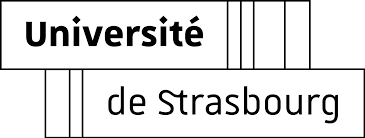
\includegraphics[height=2.2cm]{figures/lunistra}
}
\end{textblock}
\begin{textblock}{0}[0,0](13.4,0.28)
{
    \setlength{\fboxsep}{0.7pt}
    \setlength{\fboxrule}{1pt}
    \includegraphics[width=2.2cm]{logo/CNRS}
}
\end{textblock}
\small
\begin{framed}
    \vspace*{-0.7cm}
\begin{center}\textsc{Résumé}\end{center}
    \vspace*{-0.4cm}
    %Wow much physic, very nobel prize

    \textsc{Mot-clés} : %physique des particules, LHC, CMS, identification des    jets de quark beau, recherche de nouvelle physique, supersymétrie
\end{framed}
\vspace*{-0.2cm}
\begin{framed}
    \vspace*{-0.7cm}
\begin{center}\textsc{Abstract}\end{center}
    \vspace*{-0.4cm}
    %Wow much physic, very nobel prize

    \textsc{Keywords}: %particle physics, LHC, CMS, $b$-tagging, search for new    physics, supersymmetry
\end{framed}
